\documentclass[12pt,a4paper]{article}
\usepackage[utf8]{inputenc}
\usepackage[T1]{fontenc}
\usepackage{graphicx}
\usepackage{amsmath}
\usepackage{amssymb}
\usepackage{hyperref}
\usepackage{geometry}
\usepackage{fancyhdr} % For headers and footers
\usepackage{qrcode}
\usepackage{array}
\usepackage{tabularx}
\usepackage{float}
\restylefloat{figure}

\geometry{margin=1in}




\title{\vspace{-2cm} % Adjusts vertical spacing
    \includegraphics[width=3cm]{figures/contours-mindcraft-logo.png} \\ % Adds logo
    \vspace{2cm}
    Future Engineers WRO 2024 \\ \textbf{Mindcraft International Team Documentation}
}
\author{Team Members: Taha Taidi Laamiri, Salmane Derdeb \\ and Mortada Taidi Laamiri \\ Supervising Mentor: Soufiane ElHatri}
\date{\today}


\begin{document}



\maketitle




\begin{abstract}
This document provides a comprehensive overview of the design, development, and testing of our robot for the Future Engineers WRO 2024 competition. The project integrates advanced robotics concepts, innovative engineering solutions, and sustainable design practices. It details our work in hardware construction, software programming, testing, and refinement, providing an in-depth look at the Mindcraft International Team's approach and achievements.
\end{abstract}



\newpage
\tableofcontents

% Header and footer configuration
\pagestyle{fancy}
\fancyhf{}
\fancyhead[L]{Future Engineers WRO 2024 - Mindcraft International Team}
\fancyhead[R]{\thepage}
\newpage

\section{Introduction}
The Future Engineers WRO 2024 competition encourages teams to create innovative robots addressing real-world challenges through sustainable engineering and advanced technologies. The Mindcraft International Team has focused on developing an autonomous robot optimized for efficiency and reliability while adhering to the competition's sustainable development goals.

This documentation outlines our journey, from brainstorming and conceptualization to testing and final implementation. The robot was designed to navigate a complex track, detect objects, and make autonomous decisions, leveraging tools like the Raspberry Pi 4 Model B, ROS2 Humble, and custom CNC-machined parts.

Key objectives:
\begin{itemize}
    \item Develop a reliable, autonomous robot using affordable and sustainable materials.
    \item Implement modular, reusable components for easy adaptability and repair.
    \item Optimize software algorithms to ensure real-time processing and precise navigation.
    \item Integrate cutting-edge AI techniques for obstacle detection and path planning.
\end{itemize}

\newpage

\section{Team member}
Our team consists of three highly motivated and skilled individuals:
\begin{itemize}
    \item Taha TAIDI LAAMIRI
    \item Salmane DERDEB
    \item Mortada TAIDI LAAMIRI
\end{itemize}
Each member brings unique strengths and expertise, contributing to the success of the Mindcraft International Team in the Future Engineers WRO 2024 competition.

\begin{figure}[H]
    \centering
    \includegraphics[width=1\linewidth]{figures/Engineers[1].png}
    \caption{From left to right: Mortada, Taha and Salmane.}

    
\end{figure}

\newpage

\section{Design Considerations Before CAD Modeling}
Before beginning the CAD modeling process, we outlined key requirements to ensure our robot was compact, efficient, and optimized for competition challenges.

\subsection{Key Requirements}
\begin{itemize}
    \item \textbf{Compact Size}: Fit within a 20cm cube for optimal navigation.
    \item \textbf{Turning Radius}: Achieve a maximum outside turning circle of 40cm.
    \item \textbf{Stability}: Maintain a low center of gravity for balanced movement.
    \item \textbf{Weight Distribution}: Ensure equal weight distribution to prevent tipping.
    \item \textbf{High Traction}: Use high-friction wheels for better control.
    \item \textbf{Modular Assembly}: Assemble parts with screws, nuts, and zip ties—no glue.
    \item \textbf{Lightweight Design}: Reduce weight for better speed and efficiency.
    \item \textbf{Differential System}: Allow smooth and efficient turning.
    \item \textbf{Battery and Component Safety}: Position batteries securely and protect components.
    \item \textbf{Ease of Reassembly}: Design parts for easy and error-free reassembly.
\end{itemize}

\subsection{Study and Planning}
The design was meticulously planned to prioritize compactness, stability, and ease of modification. Using readily available parts ensured accessibility and reproducibility for other teams.
\newpage
\section{Initial Robot Design and Iterations}

\begin{figure}
    \centering
    \includegraphics[width=1\linewidth]{figures/Drawing/LEGO robot.png}
    \caption{LEGO robot used in the national competition.}

    
\end{figure}
\subsection{National Competition: LEGO Robot}
Our initial robot, built with LEGO components, was easy to construct but faced several limitations:
\begin{itemize}
    \item \textbf{Size and Speed Issues}: The robot was too large and slow for the competition.
    \item \textbf{Obstacle Challenges}: Difficulty in completing obstacle and parking tasks.
    \item \textbf{Structural Weaknesses}: LEGO components lacked the sturdiness needed for advanced tasks.
\end{itemize}



\subsection{First Version: Oversized DIY Robot}
After qualifying for the international stage, we decided to build a 100\% DIY robot, making all the mechanics and body ourselves while purchasing only the electronics. The first version was oversized and heavy, impacting speed and maneuverability.

\subsection{Second Version: Lack of Differential System}
In the second iteration of our DIY robot, we reduced the size and weight but encountered new challenges:
\begin{itemize}
    \item \textbf{No Differential System}: Turning was inefficient, requiring a 150cm radius to complete a full turn.
    \item \textbf{Inefficient Design}: Poor handling prevented precise movements required for competition.
\end{itemize}

\subsection{Third Version: Final Optimized Robot}
The third version incorporated all lessons learned:
\begin{itemize}
    \item \textbf{Compact Design}: Fits within a 20cm cube.
    \item \textbf{Differential System}: Enabled efficient turning within a 40cm radius.
    \item \textbf{Hardware Upgrade}: Switched to Raspberry Pi 4B for better compatibility, reduced weight, and energy efficiency.
    \item \textbf{Modular Assembly}: Assembled with screws and zip ties for easy modifications.
    \item \textbf{Safety Features}: Secured battery placement and protected components.
\end{itemize}

\begin{figure}[ht]
    \centering
    \includegraphics[width=1\textwidth]{figures/Drawing/DIY ROBOT.jpeg}
    \caption{Final optimized robot design.}
    \label{fig:final_robot}
\end{figure}

\section{3D CAD Modeling}
\subsection{Why We Chose Onshape}
\begin{itemize}
    \item \textbf{Cloud-Based Collaboration}: Allowed team members to work simultaneously from different locations.
    \item \textbf{Free for Educational Use}: Eliminated software costs while providing advanced CAD features.
    \item \textbf{Accessible Anywhere}: Runs in a browser, making it hardware-independent.
    \item \textbf{Powerful CAD Tools}: Provided tools for creating complex mechanical components.
\end{itemize}

\begin{figure}[ht]
    \centering
    \includegraphics[width=0.5\linewidth]{figures/onshape.png}
    \caption{Onshape logo.}
    \label{fig:onshape}
\end{figure}


\begin{figure}[ht]
    \centering
    \includegraphics[width=1\linewidth]{figures/isometric Pic/robot base.png}
    \caption{3D model of the robot in Onshape.}
    \label{fig:onshape_model}
\end{figure}

\subsection{CAD Features and Outputs}
The CAD design included:
\begin{itemize}
    \item Steering system linkages for precise control.
    \item Differential gear systems for efficient power transfer.
    \item Custom chassis mounts and supports for modular assembly.
\end{itemize}

\section{3D Printing}
\subsection{Why 3D Printing?}
\begin{itemize}
    \item Enables creation of complex geometries not feasible with other methods.
    \item Supports rapid prototyping for iterative design improvements.
    \item Cost-effective and generates less material waste.
\end{itemize}

\subsection{Creality K1 Max}
We used the Creality K1 Max for its:
\begin{itemize}
    \item \textbf{Large Build Volume}: Allowed printing of large components in a single piece.
    \item \textbf{High Speed}: Enabled fast production of prototypes.
    \item \textbf{Precision}: Ensured parts fit together seamlessly.
\end{itemize}

\begin{figure}[ht]
    \centering
    \includegraphics[width=0.5\textwidth]{figures/creality.png}
    \caption{Creality K11 Max.}
    \label{fig:creality}
\end{figure}


\begin{figure}[ht]
    \centering
    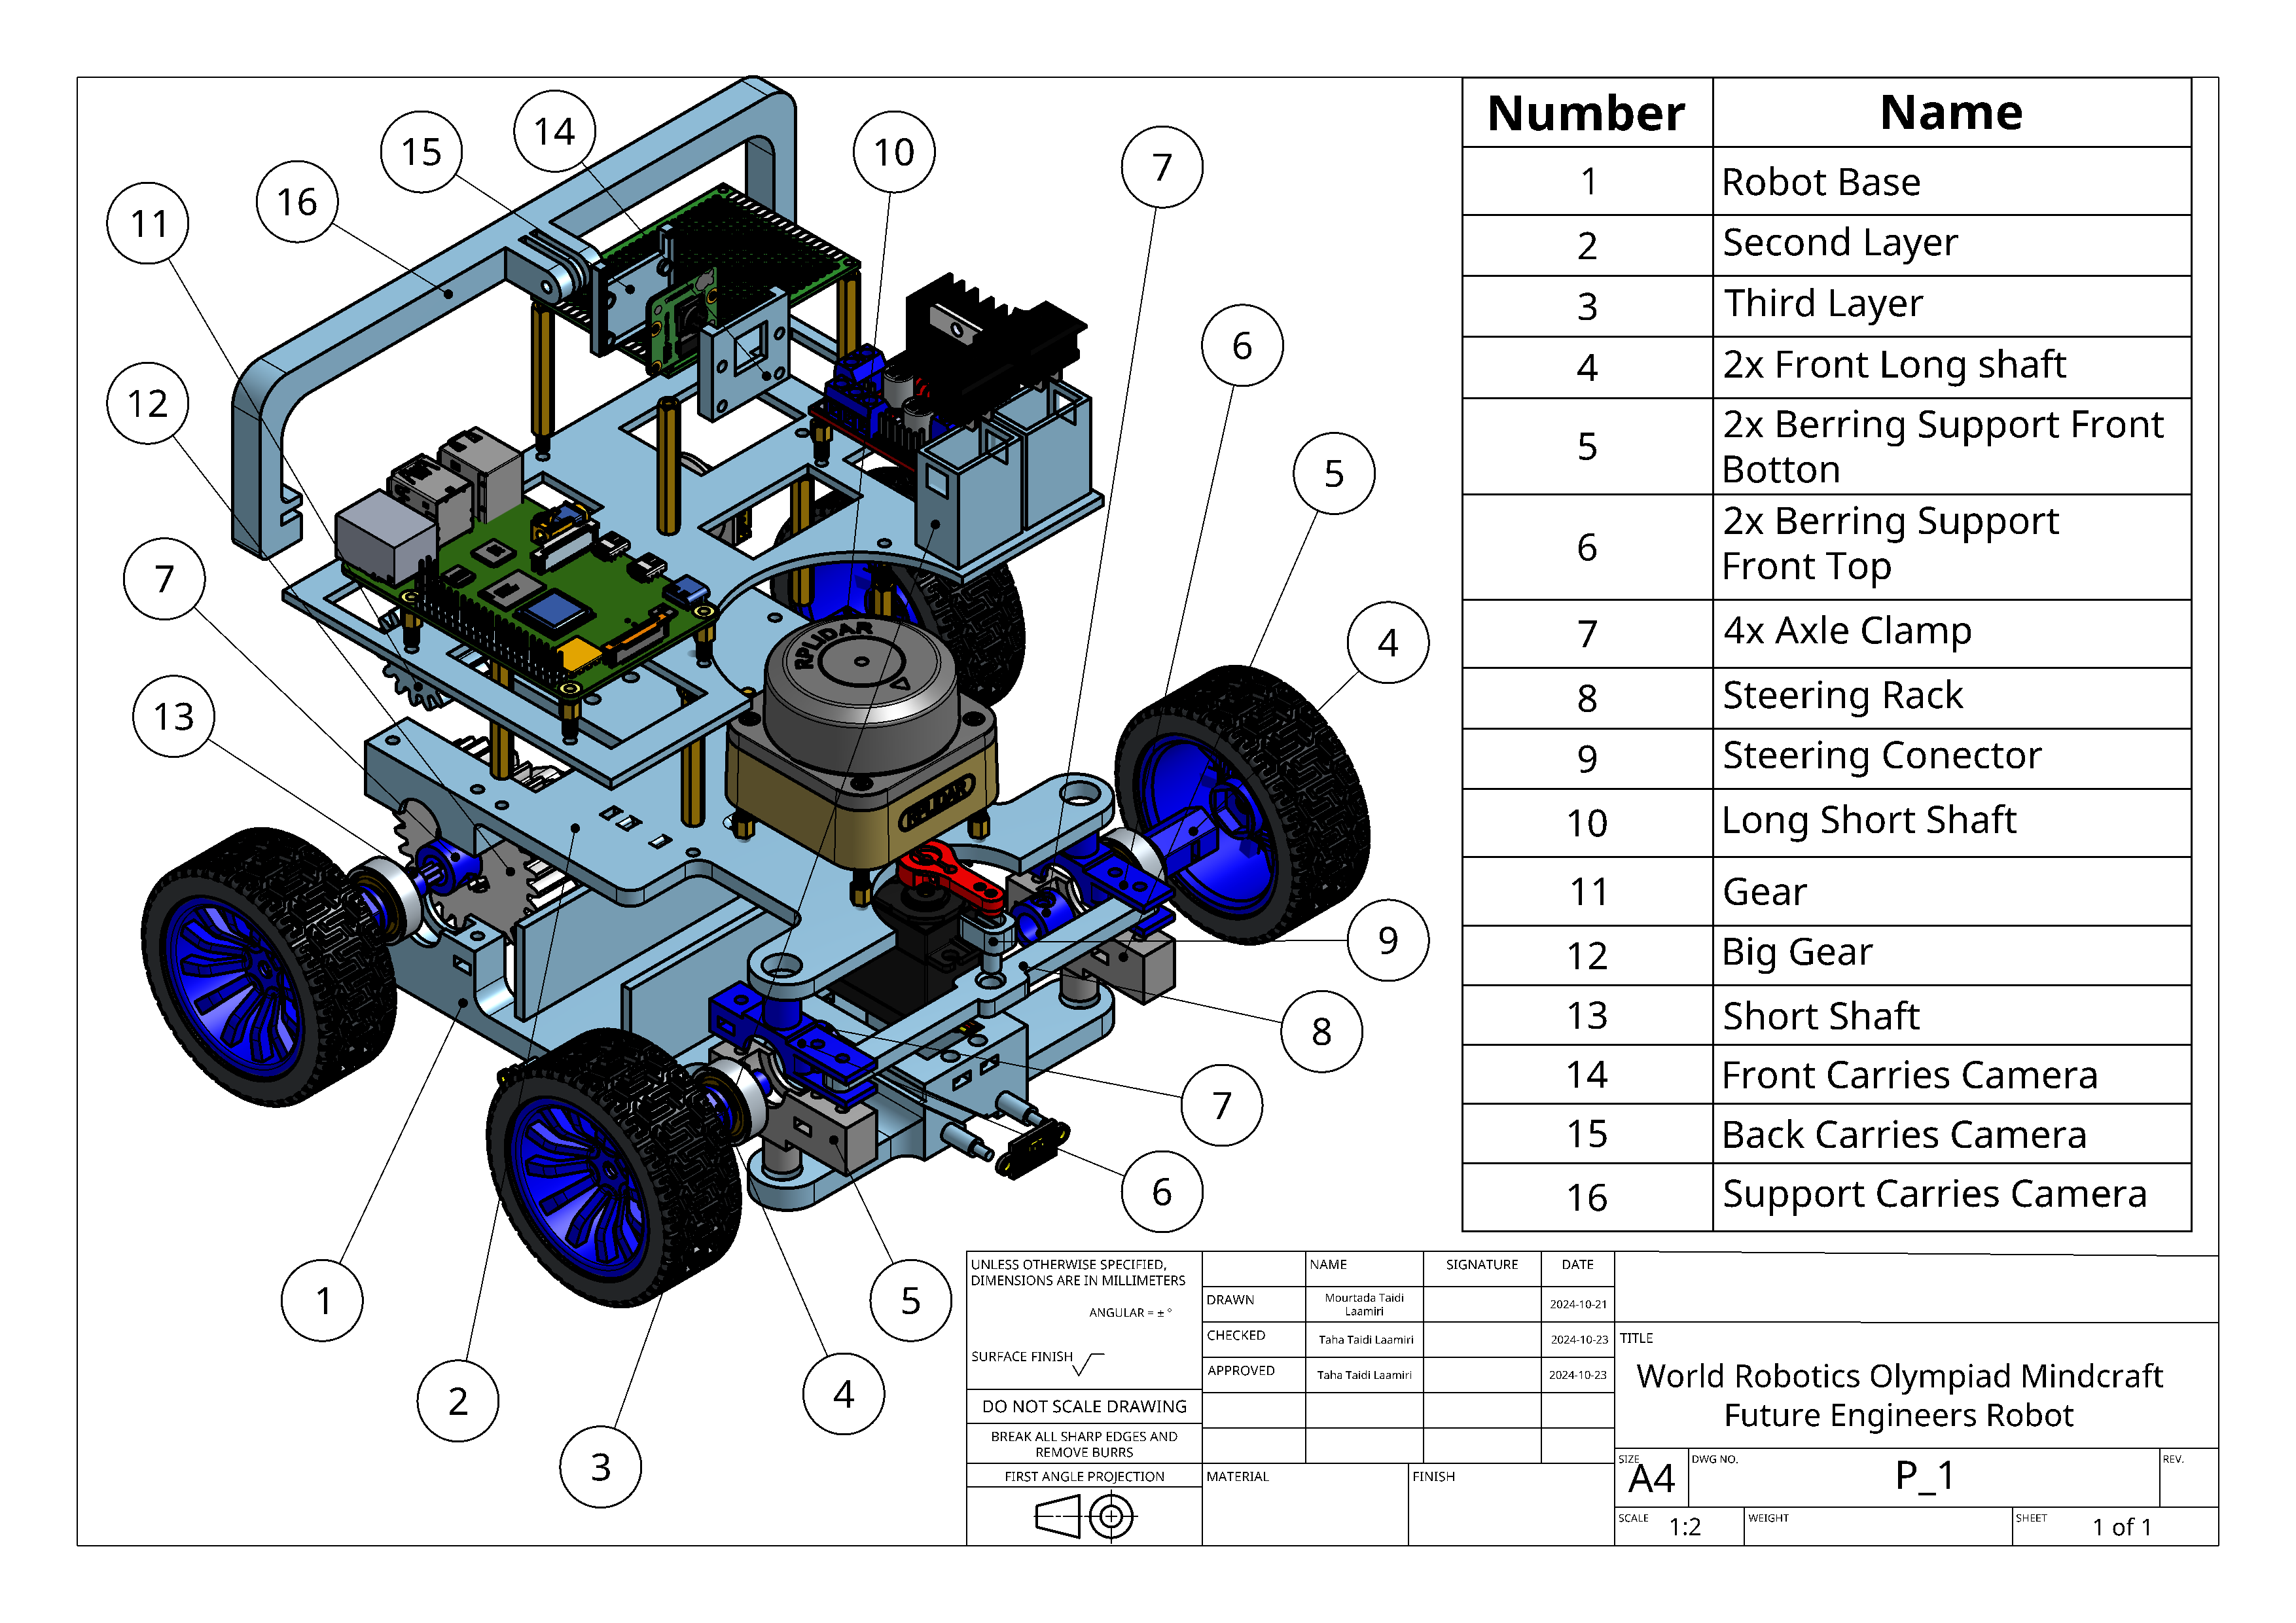
\includegraphics[width=1\textwidth]{figures/Drawing/Drawing Parts Robot.png}
    \caption{3D printed parts for the robot.}
    \label{fig:printed_parts}
\end{figure}

\section{Robot Parts Details}
The following table lists the robot's custom-designed and printed components:

\begin{table}
    \centering
    \begin{tabular}{|l|l|}
        \hline
        \textbf{Part Name} & \textbf{Description} \\ \hline
        Robot Base & Foundation of the chassis. \\ \hline
        Steering Rack & Enables precise turning control. \\ \hline
        Camera Mount & Holds the vision system securely. \\ \hline
        Differential Gears & Transmits power efficiently to wheels. \\ \hline
        Motor Mount & Secures the motors in place. \\ \hline
    \end{tabular}
    \caption{List of key robot components.}
    \label{tab:robot_parts}
\end{table}



\newpage


\section*{Bill of Materials}

\renewcommand{\arraystretch}{1.5} % Adjust row height for readability

\setlength{\extrarowheight}{2pt}  % Additional row spacing

\begin{tabularx}{\textwidth}{|l|X|X|X|}
\hline
\textbf{Code} & \textbf{Name} & \textbf{Description} & \textbf{Image} \\
\hline
0x00 & Raspberry Pi 4B & Main computing unit & 
\includegraphics[width=3cm]{figures/BOM/WRO-FE/Rpf-raspberry-pi-4-model-b.png} \\
\hline
0x01 & Arduino Nano & Microcontroller & 
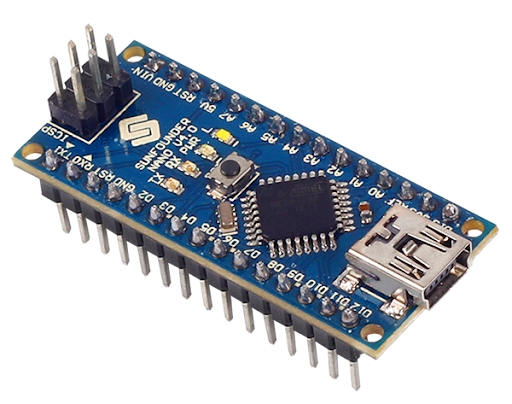
\includegraphics[width=3cm]{figures/BOM/WRO-FE/arduino NANO.png} \\
\hline

\end{tabularx}


\newpage


\section*{}

\begin{tabularx}{\textwidth}{|l|X|X|X|}
\hline
0x02 & RPLidar C1 & LiDAR sensor for object detection & 
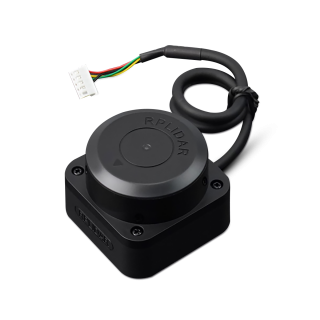
\includegraphics[width=2.5cm]{figures/BOM/WRO-FE/LIDAR.png} \\
\hline
0x03 & VL53L1X Sensor & Time-of-flight distance sensor & 
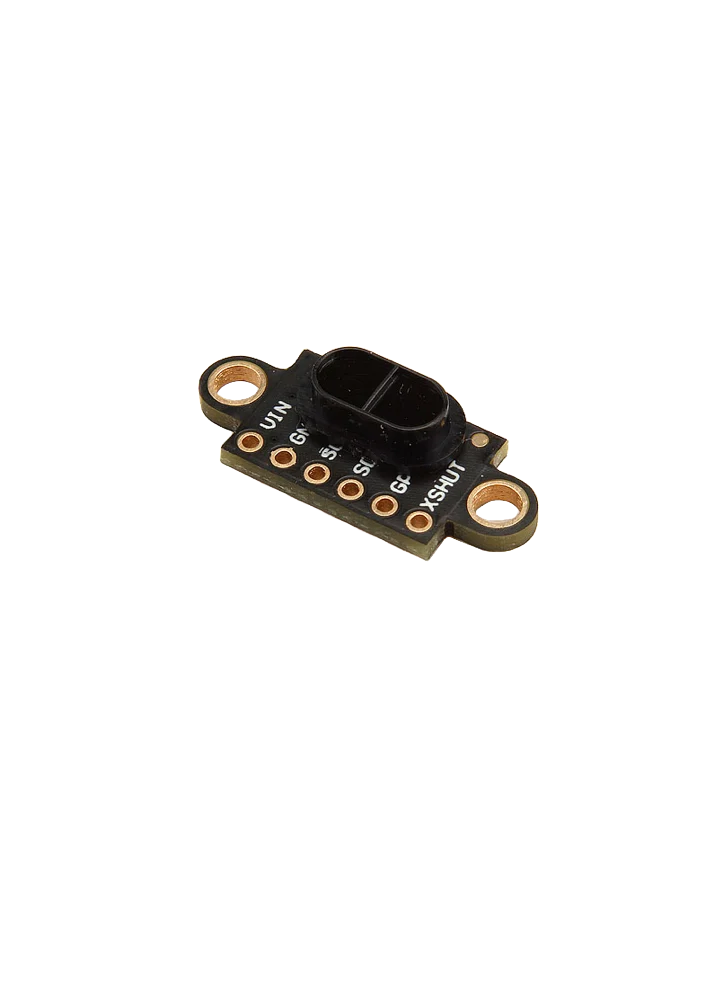
\includegraphics[width=3cm]{figures/BOM/WRO-FE/VLX1-DTOF.png} \\
\hline
0x04 & Gyroscope Sensor & Measures angular velocity & 
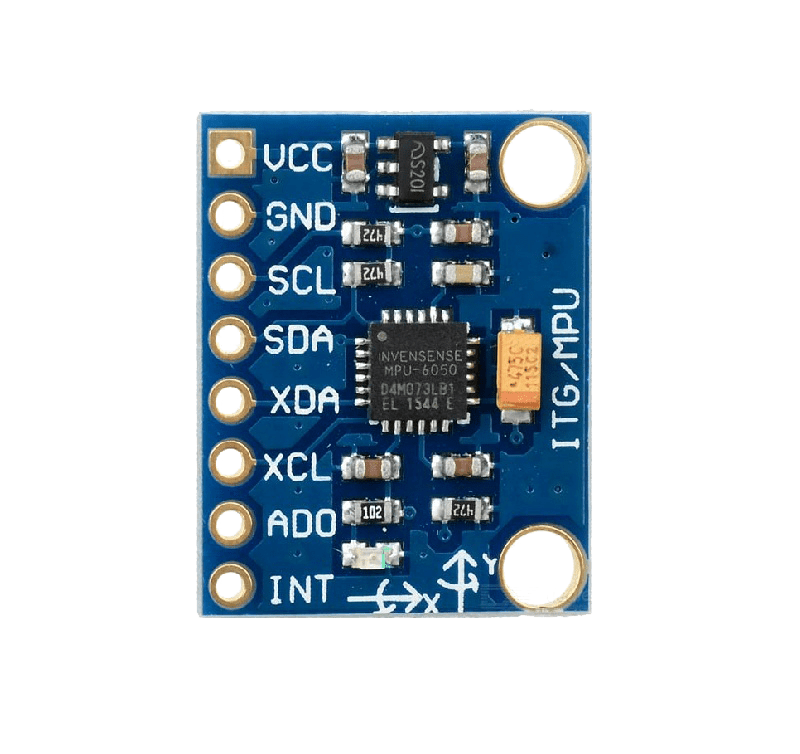
\includegraphics[width=2.5cm]{figures/BOM/WRO-FE/mpu-6050.png} \\
\hline
0x05 & Raspberry Pi Camera Module 3 Wide & Captures video for color detection & 
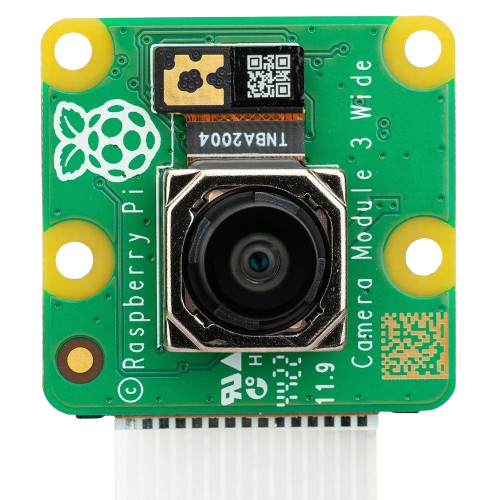
\includegraphics[width=2.5cm]{figures/BOM/WRO-FE/CAM-RASPI.png} \\
\hline
0x06 & DC Brushed Motor with Encoder & Motor for movement with encoder feedback & 
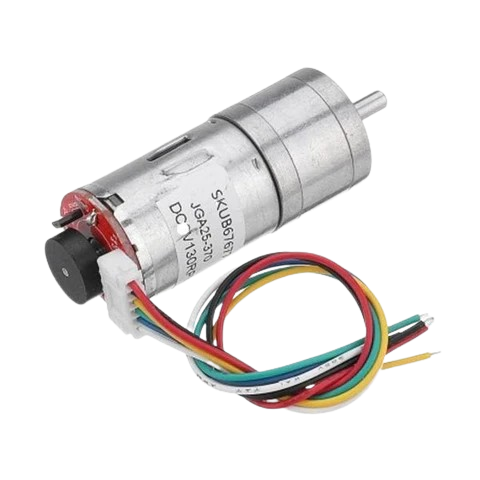
\includegraphics[width=2.5cm]{figures/BOM/WRO-FE/Brushed motor.png} \\
\hline
0x07 & Wheels & Wheels for robot movement & 
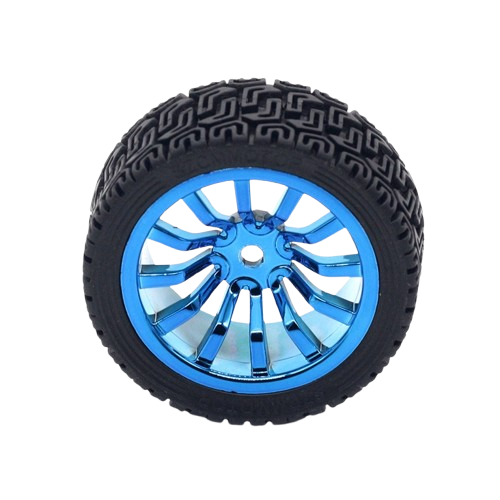
\includegraphics[width=2.5cm]{figures/BOM/WRO-FE/Wheels.png} \\
\hline
0x08 & L298 Motor Driver & Command Motor High Voltage with logic voltage 5v & 
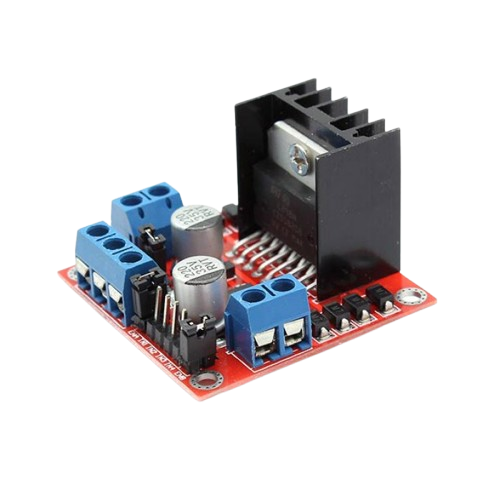
\includegraphics[width=2.5cm]{figures/BOM/WRO-FE/Driver.png} \\
\hline

\end{tabularx}

\newpage

\section*{}

\begin{tabularx}{\textwidth}{|l|X|X|X|}

\hline

0x09 & Servo motor Metal Gear Box 180° & For Robot turning & 
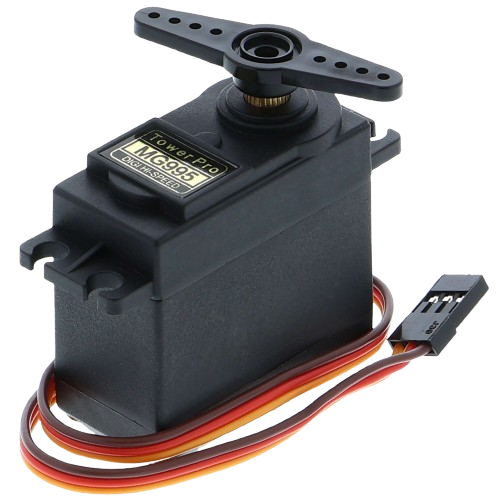
\includegraphics[width=2.5cm]{figures/BOM/WRO-FE/SERVO.png} \\
\hline
0x10 & 5V Power Converter & 5V Power Converter & 
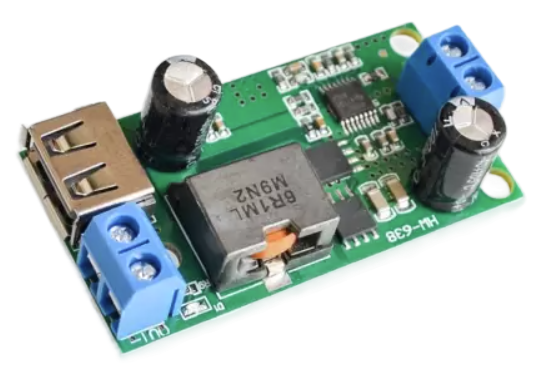
\includegraphics[width=2.5cm]{figures/BOM/WRO-FE/5V.png} \\
\hline
0x11 & 5V Lipo 3S 2200mah 11.1V 50C & Lithium Polymer Battery & 
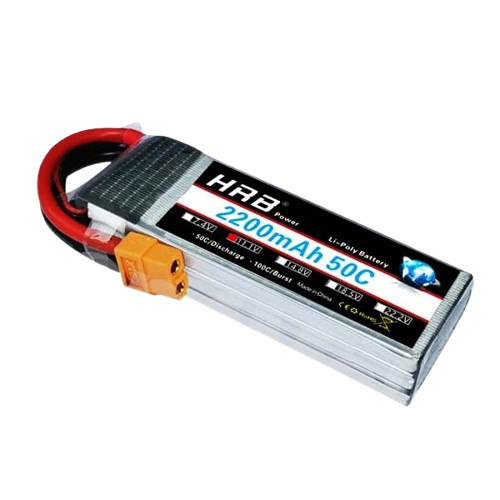
\includegraphics[width=2.5cm]{figures/BOM/WRO-FE/BATTERIE.png} \\
\hline
0x12 & IMAX B6AC V2 & Battery Charger & 
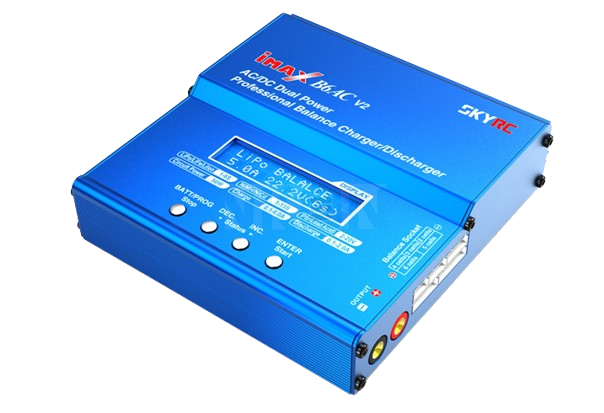
\includegraphics[width=3cm]{figures/BOM/WRO-FE/B6AC1.png} \\
\hline
0x13 & 7806 Transistor & 6V Voltage Regulator & 
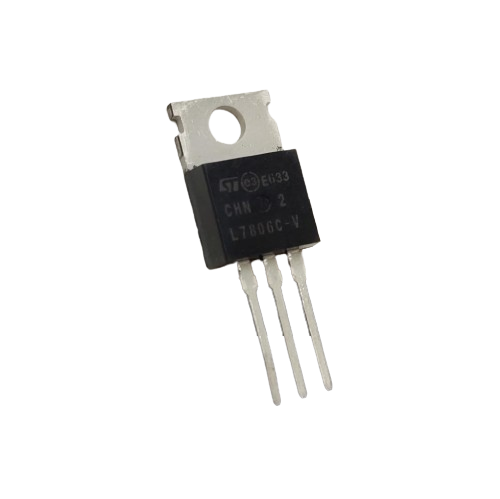
\includegraphics[width=2.5cm]{figures/BOM/WRO-FE/TRANSISTORS.png} \\
\hline
0x14 & Switch High Amper & High Current Switch & 
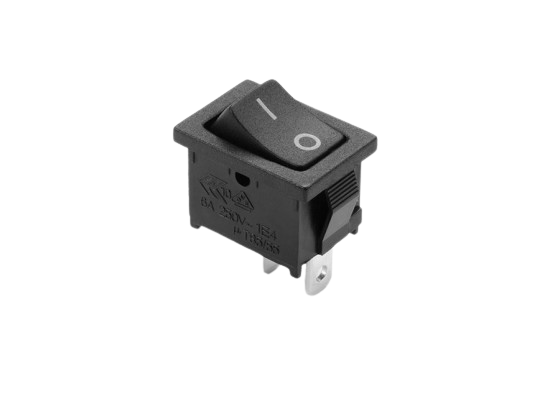
\includegraphics[width=2.5cm]{figures/BOM/WRO-FE/Switch.png} \\
\hline
0x15 & 	Buzzer Alarm Batterie Lipo & Lipo Battery Alarm	 & 
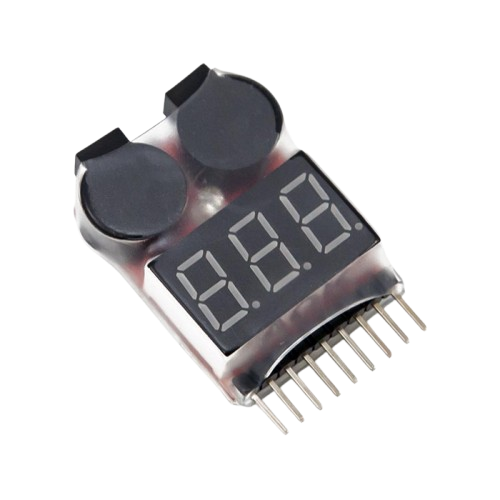
\includegraphics[width=2.5cm]{figures/BOM/WRO-FE/BATTERY (2).png} \\
\hline

0x16 & Servo Tester & Servo Motor Tester & 
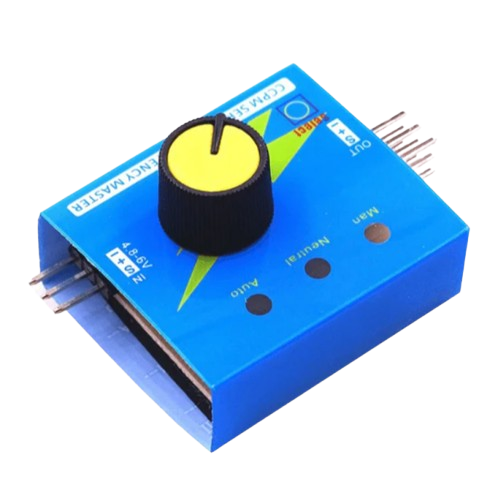
\includegraphics[width=2.5cm]{figures/BOM/WRO-FE/pwm.png} \\
\hline
0x17 & 	Servobras & Servo Arm & 
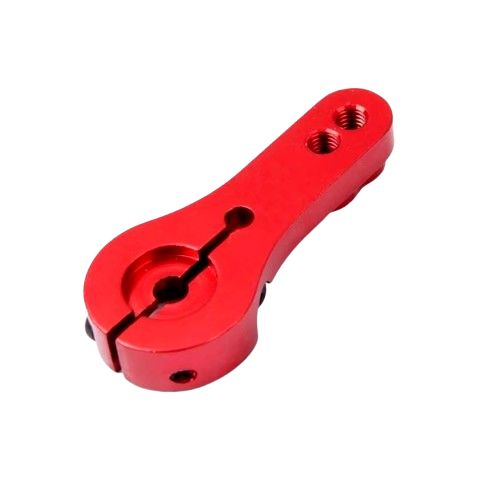
\includegraphics[width=2.5cm]{figures/BOM/WRO-FE/SERVOBRAS.png} \\
\hline
\end{tabularx}


\newpage

\section*{}

\begin{tabularx}{\textwidth}{|l|X|X|X|}
\hline
0x18 & SD Card 64GB & 64GB SD Card & 
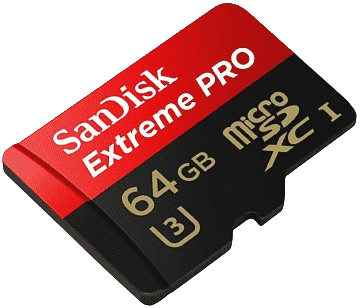
\includegraphics[width=2.5cm]{figures/BOM/WRO-FE/MEMORY-CARD.png} \\
\hline
\end{tabularx}

\begin{figure}[H]
    \centering
    \caption{List of materials (BOM List)}
    \label{fig:bom}
\end{figure}

\newpage

\begin{figure}[H]
    \vspace{4cm}
    \centering
    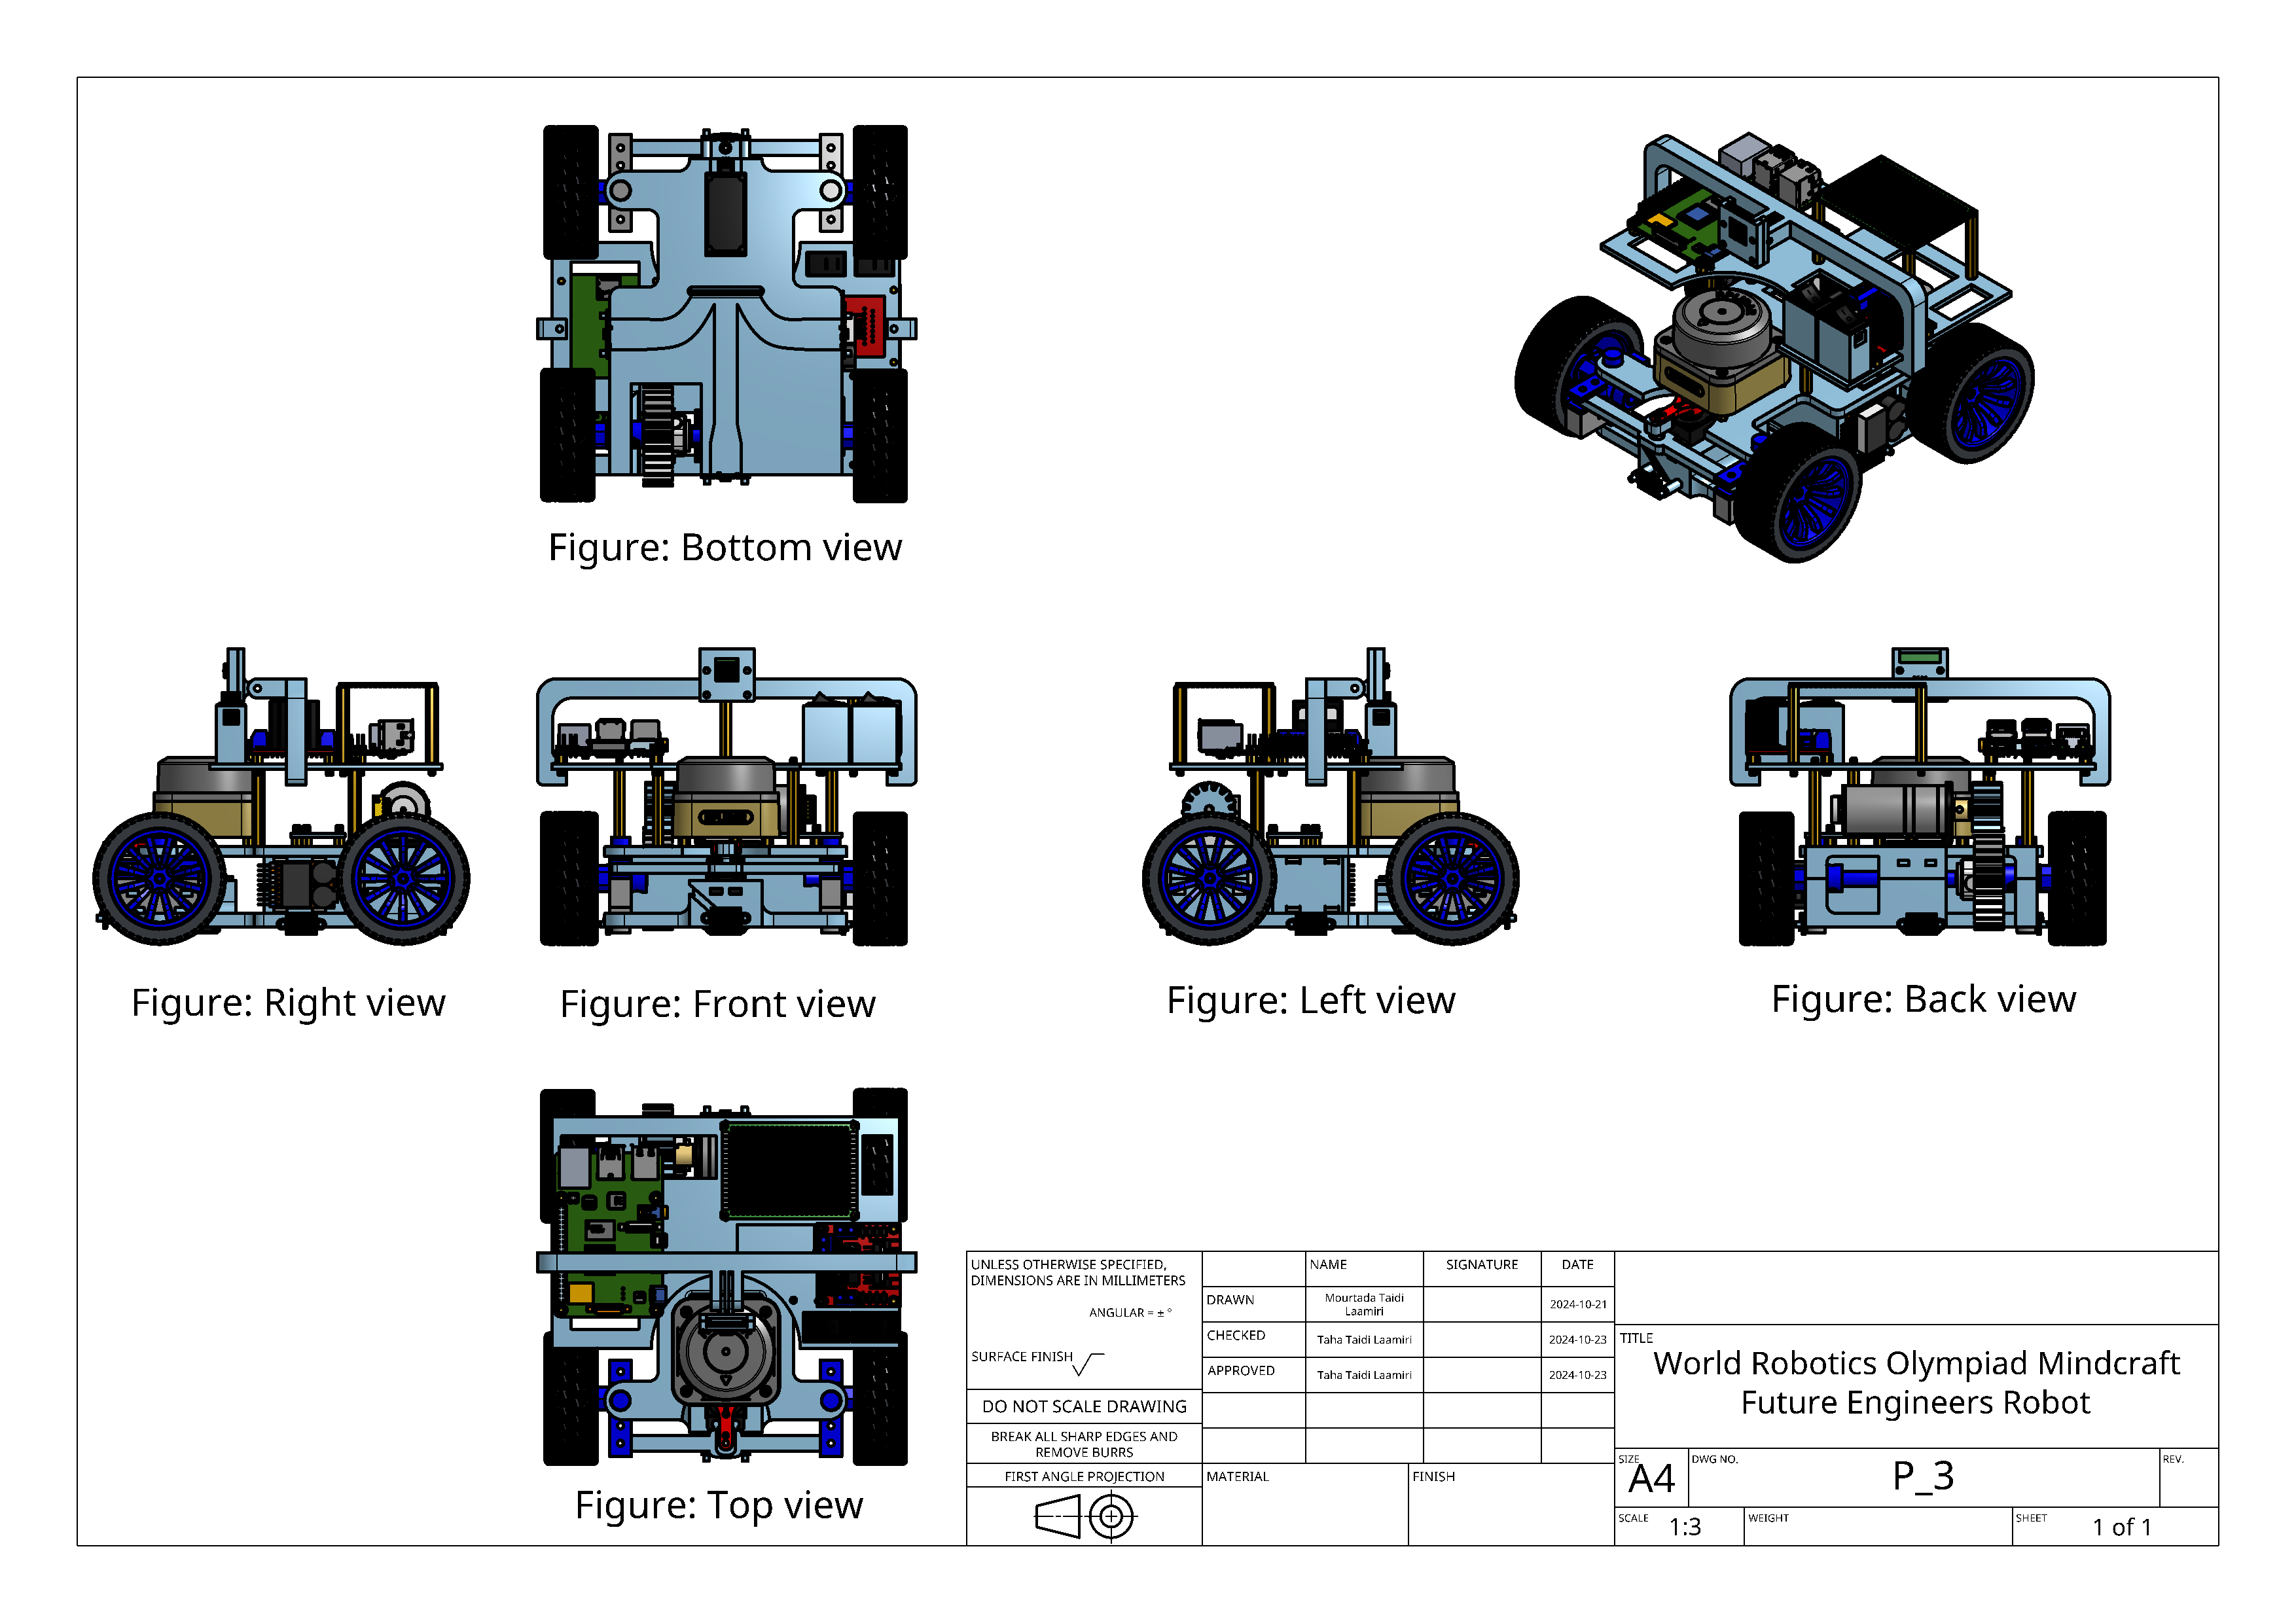
\includegraphics[width=\textwidth, angle=90]{figures/Drawing/Drawing Views Robot.png}
    \caption{Robot Views}
\end{figure}

\begin{figure}[H]
    \vspace{4cm}
    \centering
    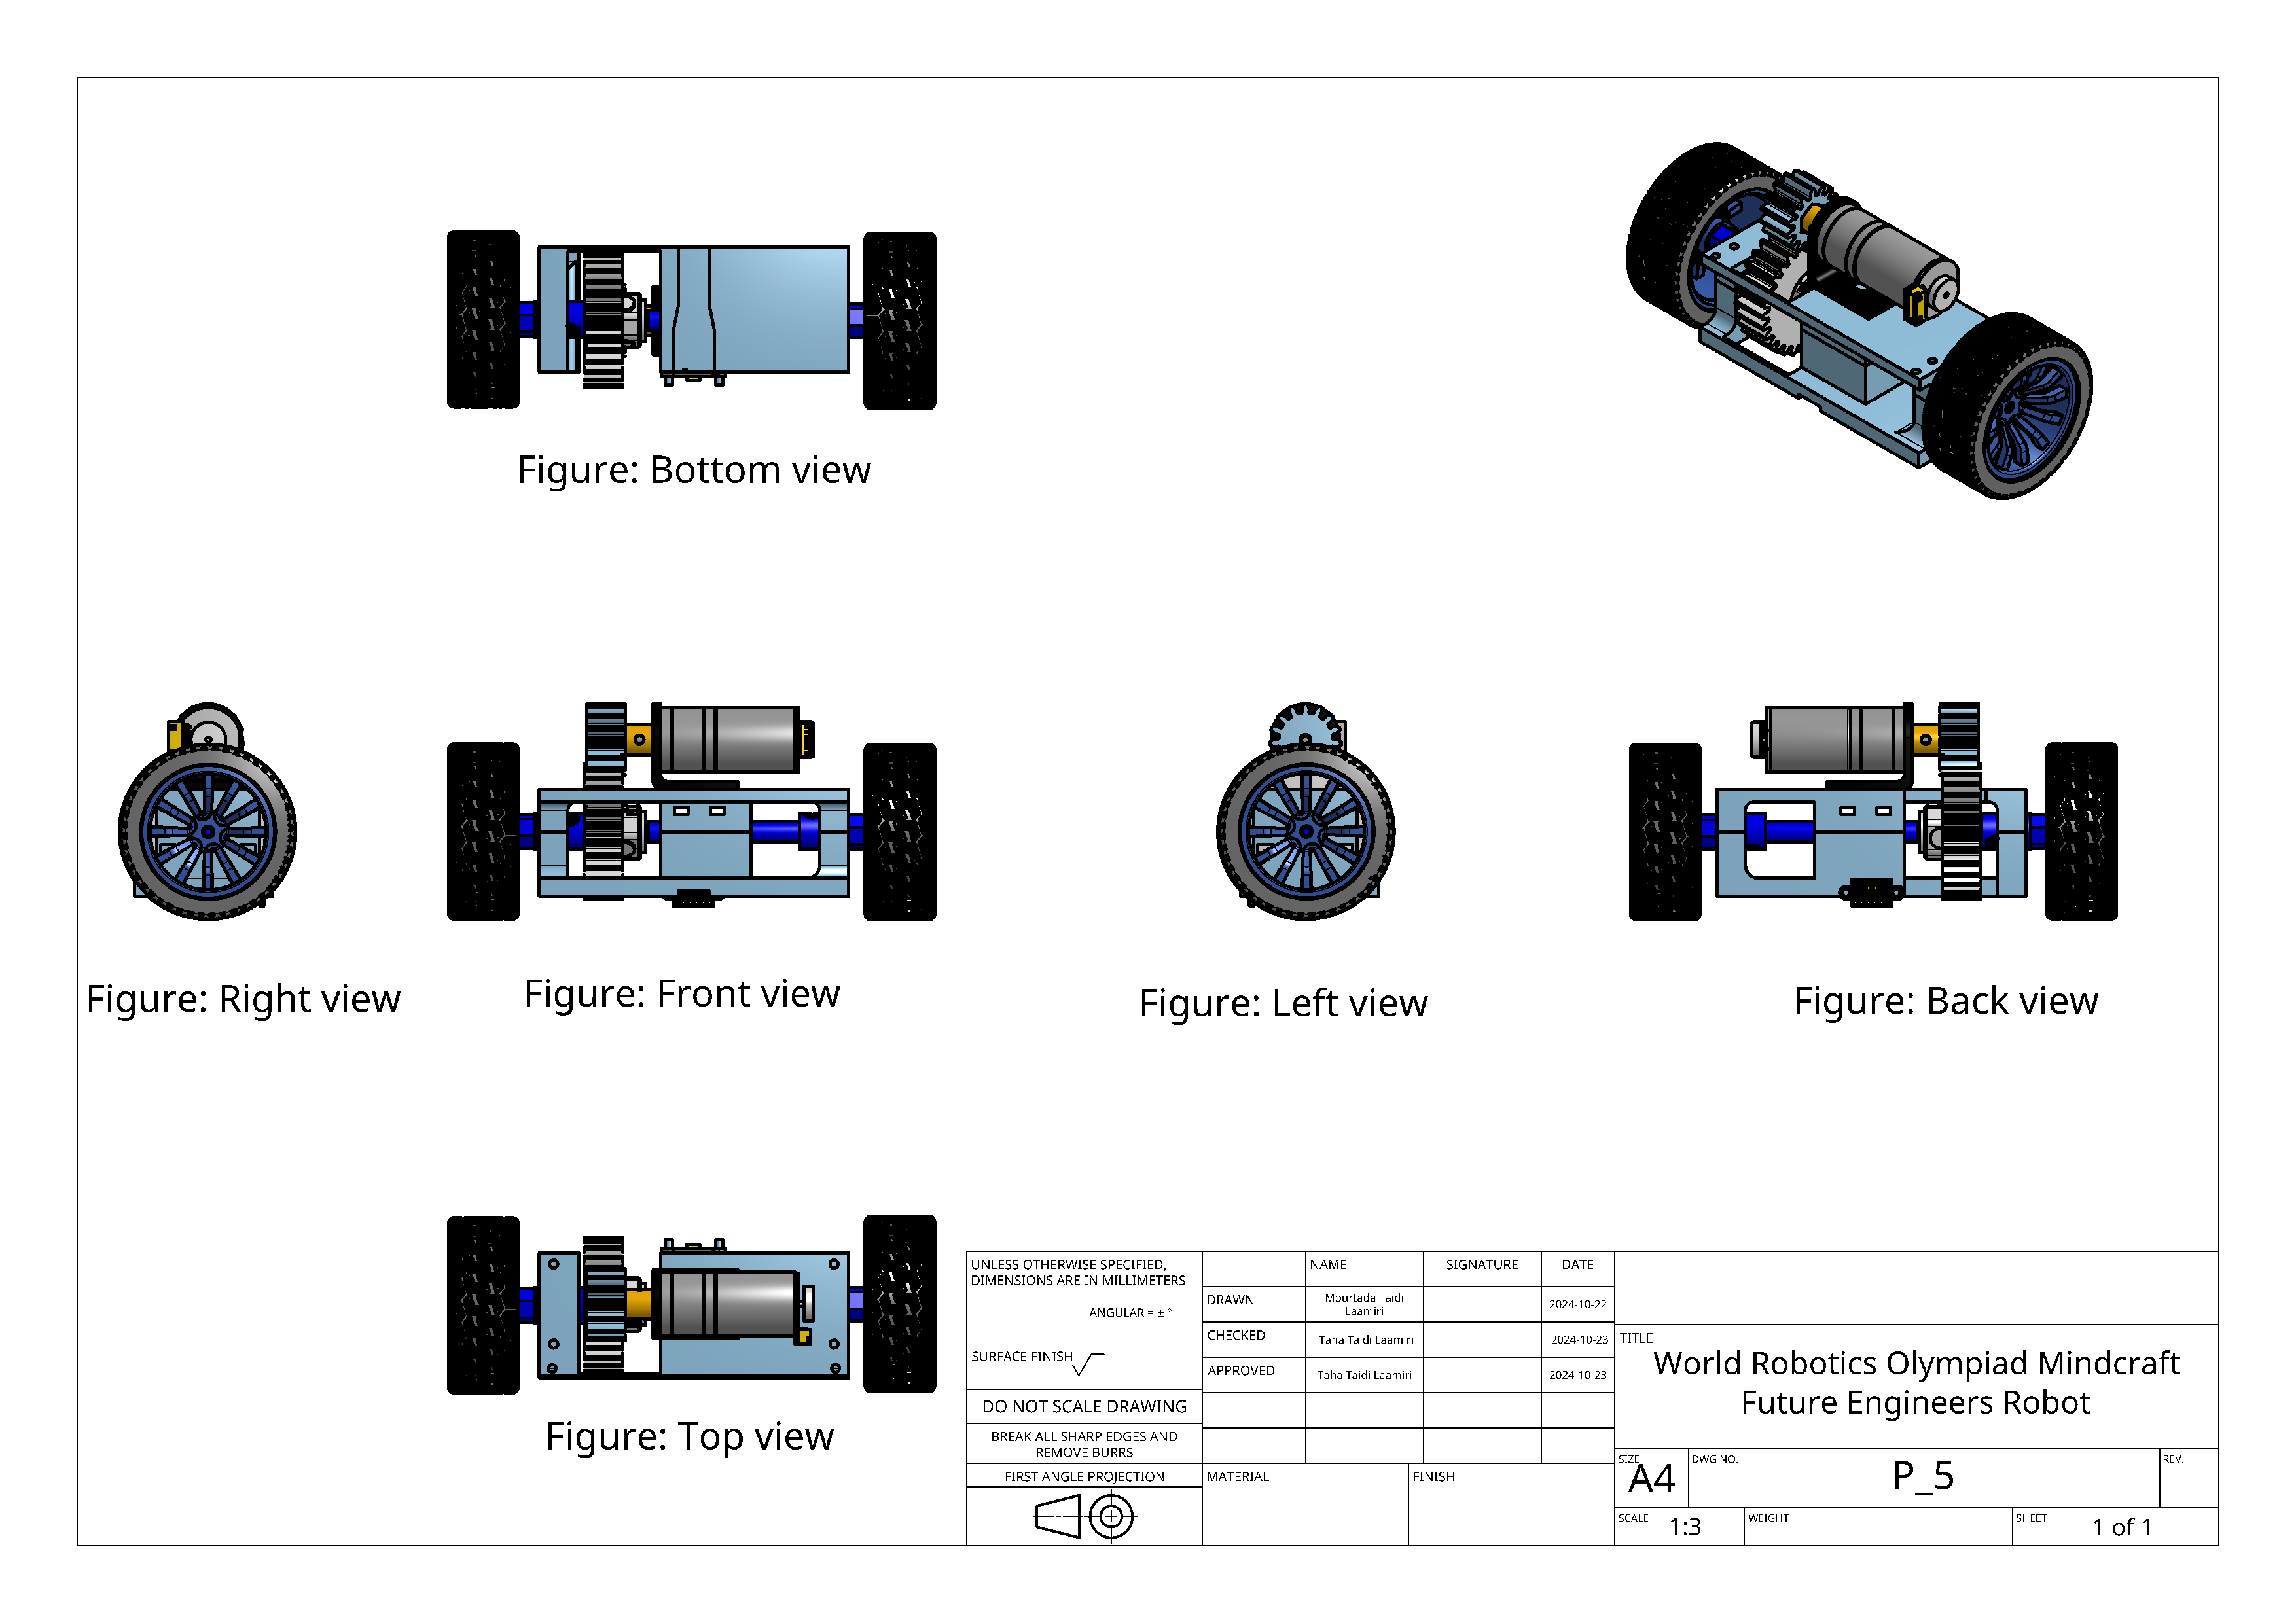
\includegraphics[width=\textwidth, angle=90]{figures/Drawing/Drawing Assembly Power.png}
    \caption{Assembly Power}
\end{figure}

\begin{figure}[H]
    \vspace{4cm}
    \centering
    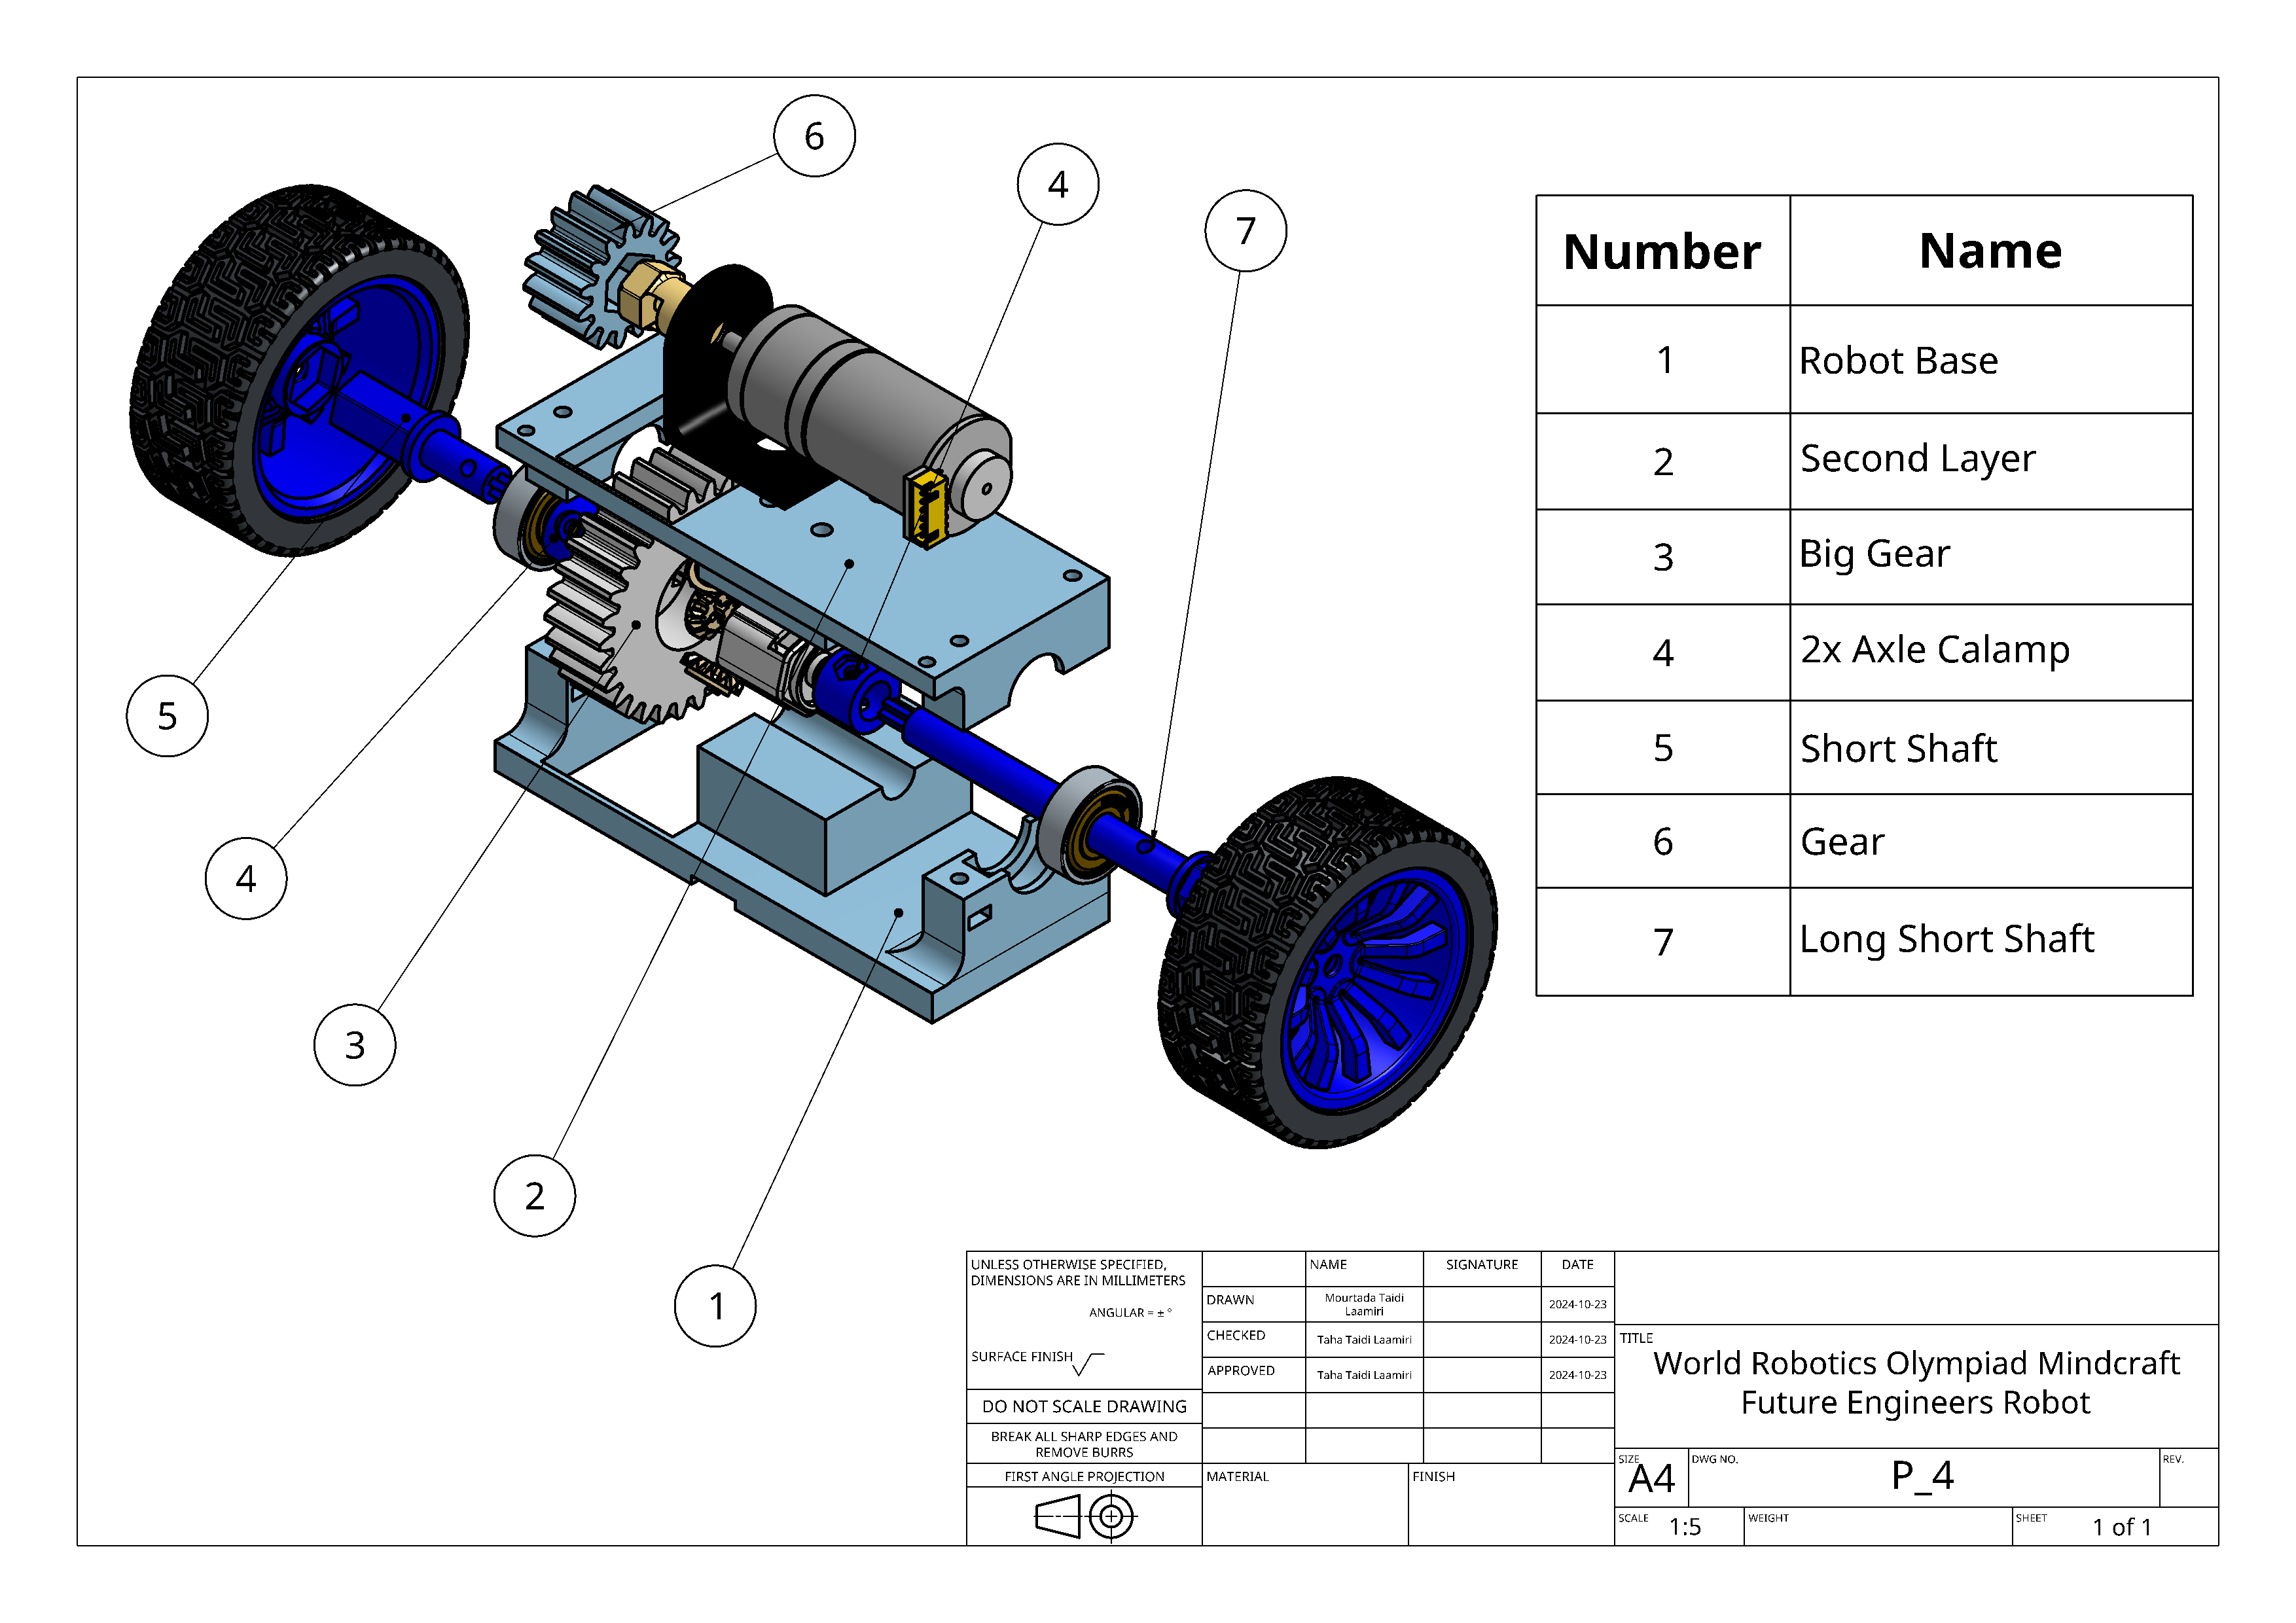
\includegraphics[width=\textwidth, angle=90]{figures/Drawing/Drawing Assembly Power Animation.png}
    \caption{Assembly Power Animation}
\end{figure}

\begin{figure}[H]
    \vspace{4cm}
    \centering
    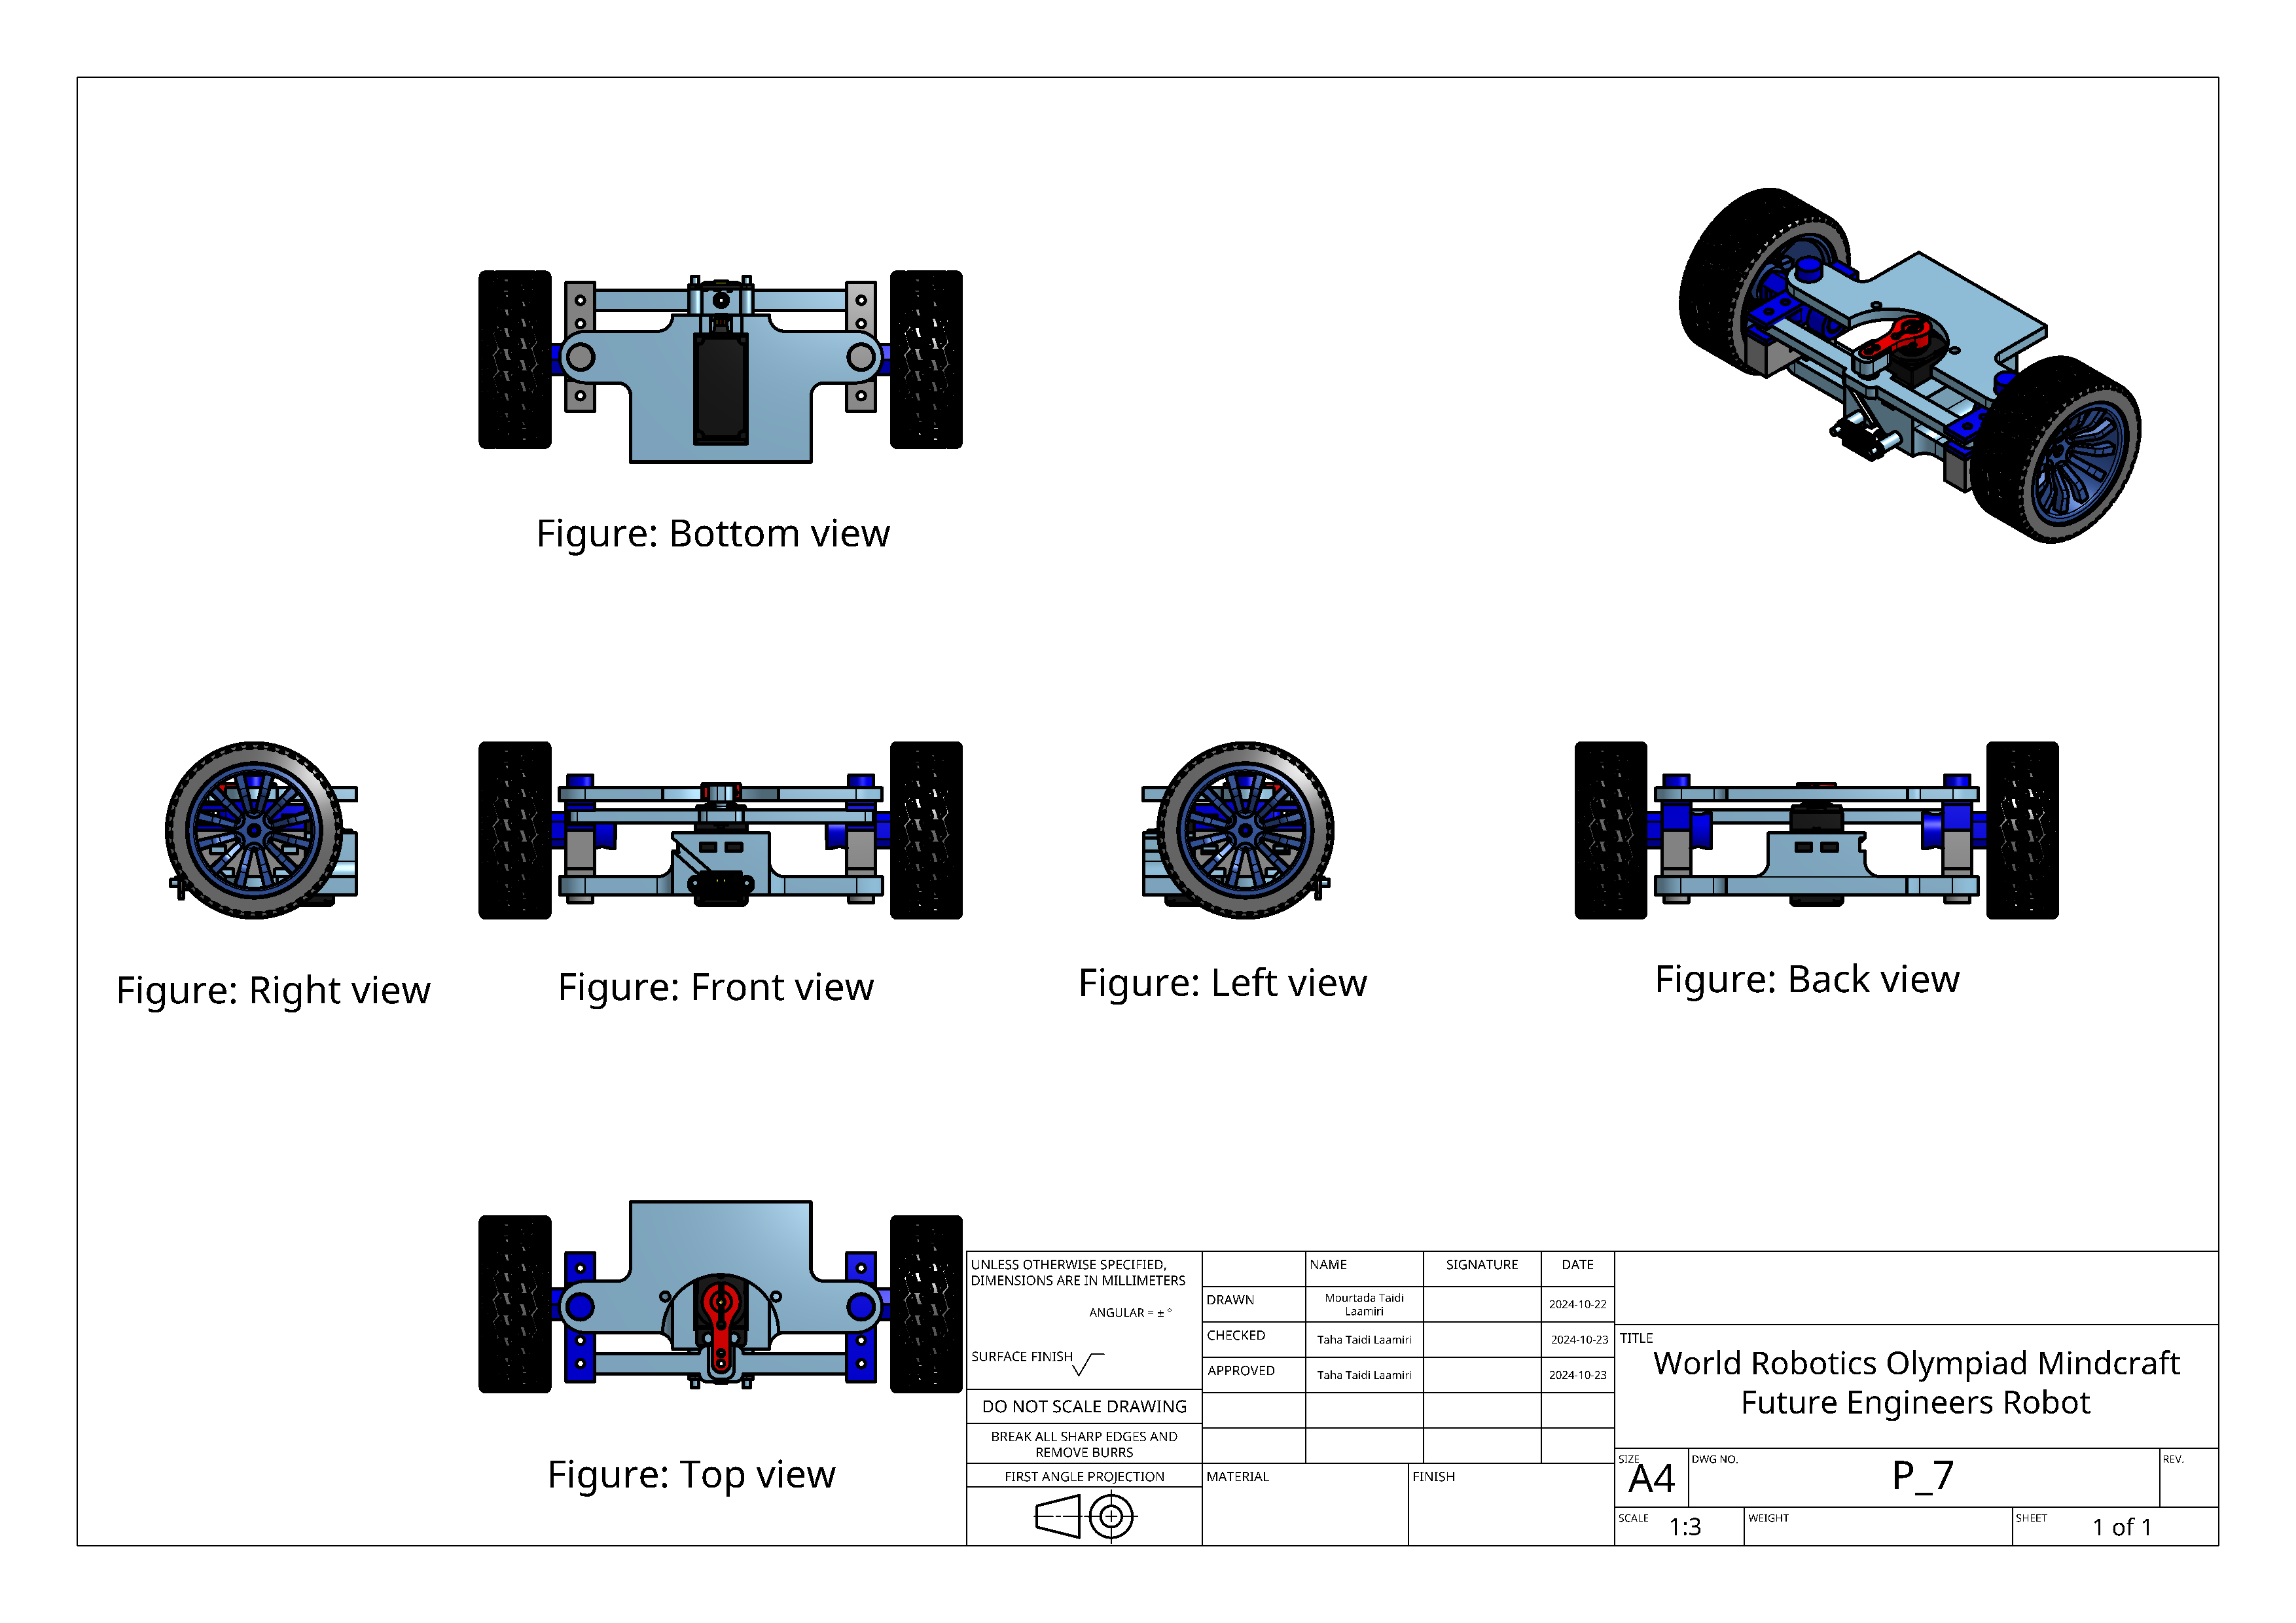
\includegraphics[width=\textwidth, angle=90]{figures/Drawing/Drawing Assembly Steering.png}
    \caption{Assembly Steering}
\end{figure}

\begin{figure}[H]
    \vspace{4cm}
    \centering
    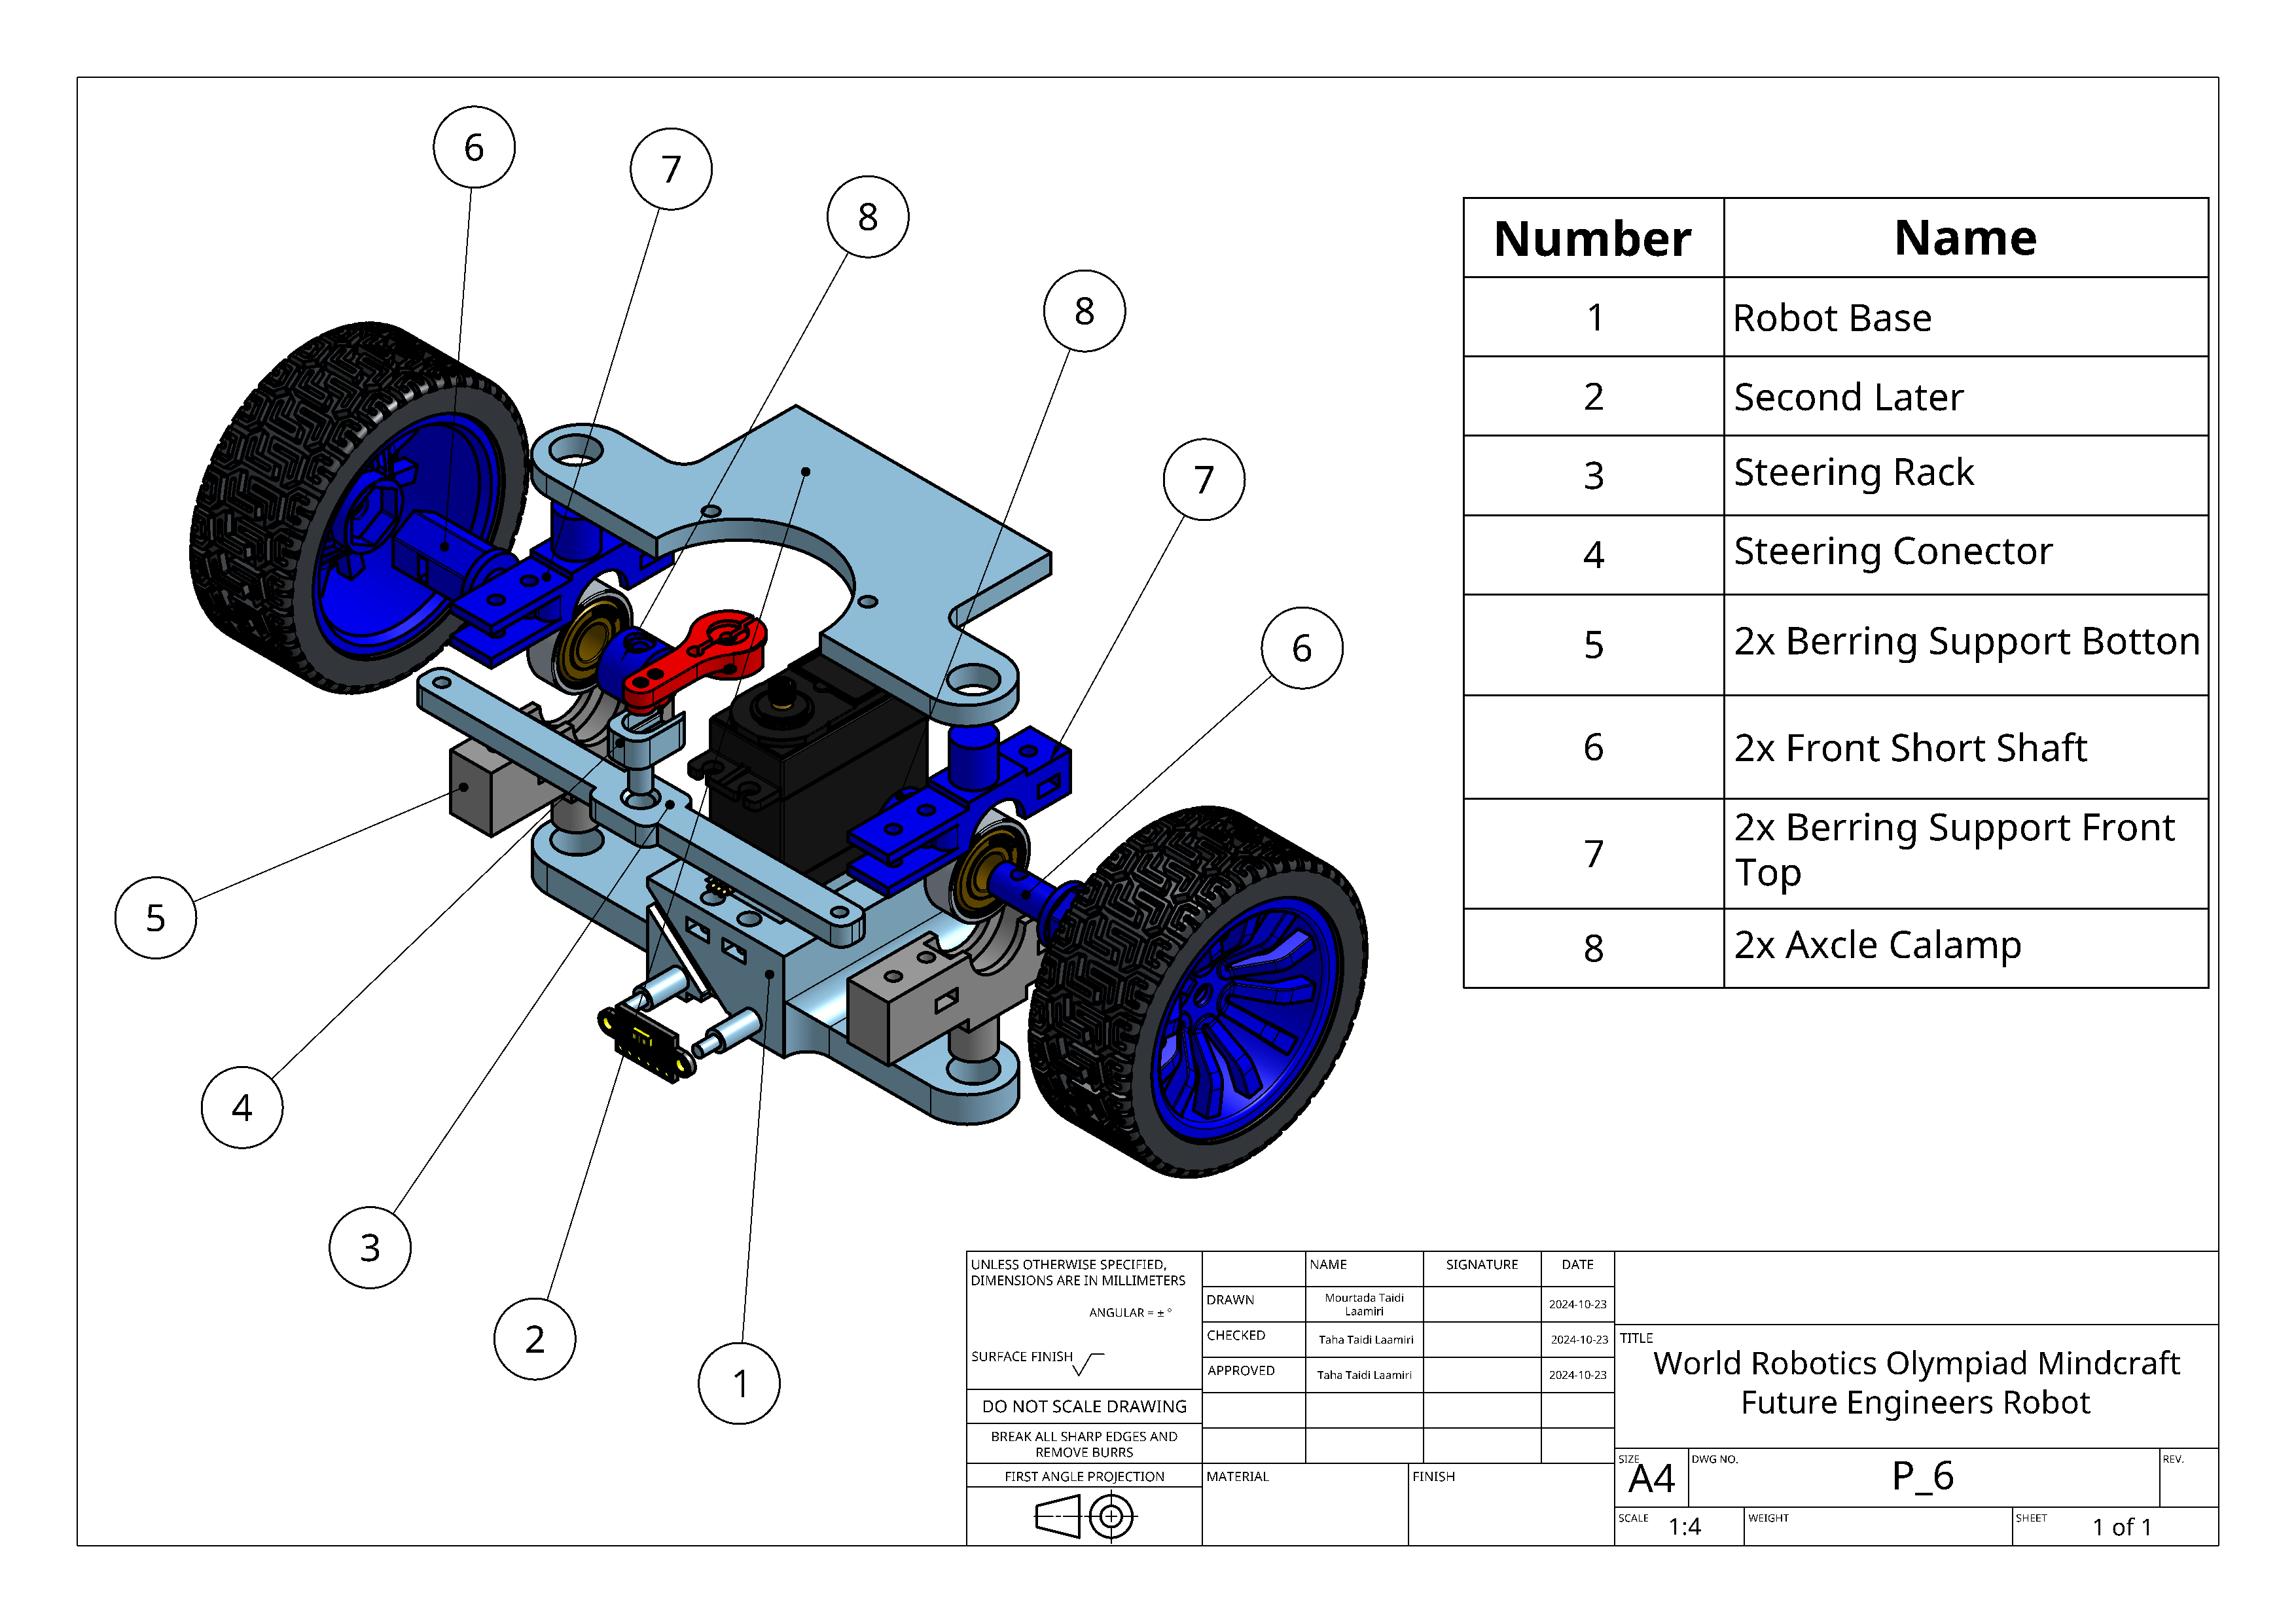
\includegraphics[width=\textwidth, angle=90]{figures/Drawing/Drawing Assembly Steering Animation.png}
    \caption{Assembly Steering Animation}
\end{figure}

\begin{figure}[H]
    \vspace{4cm}
    \centering
    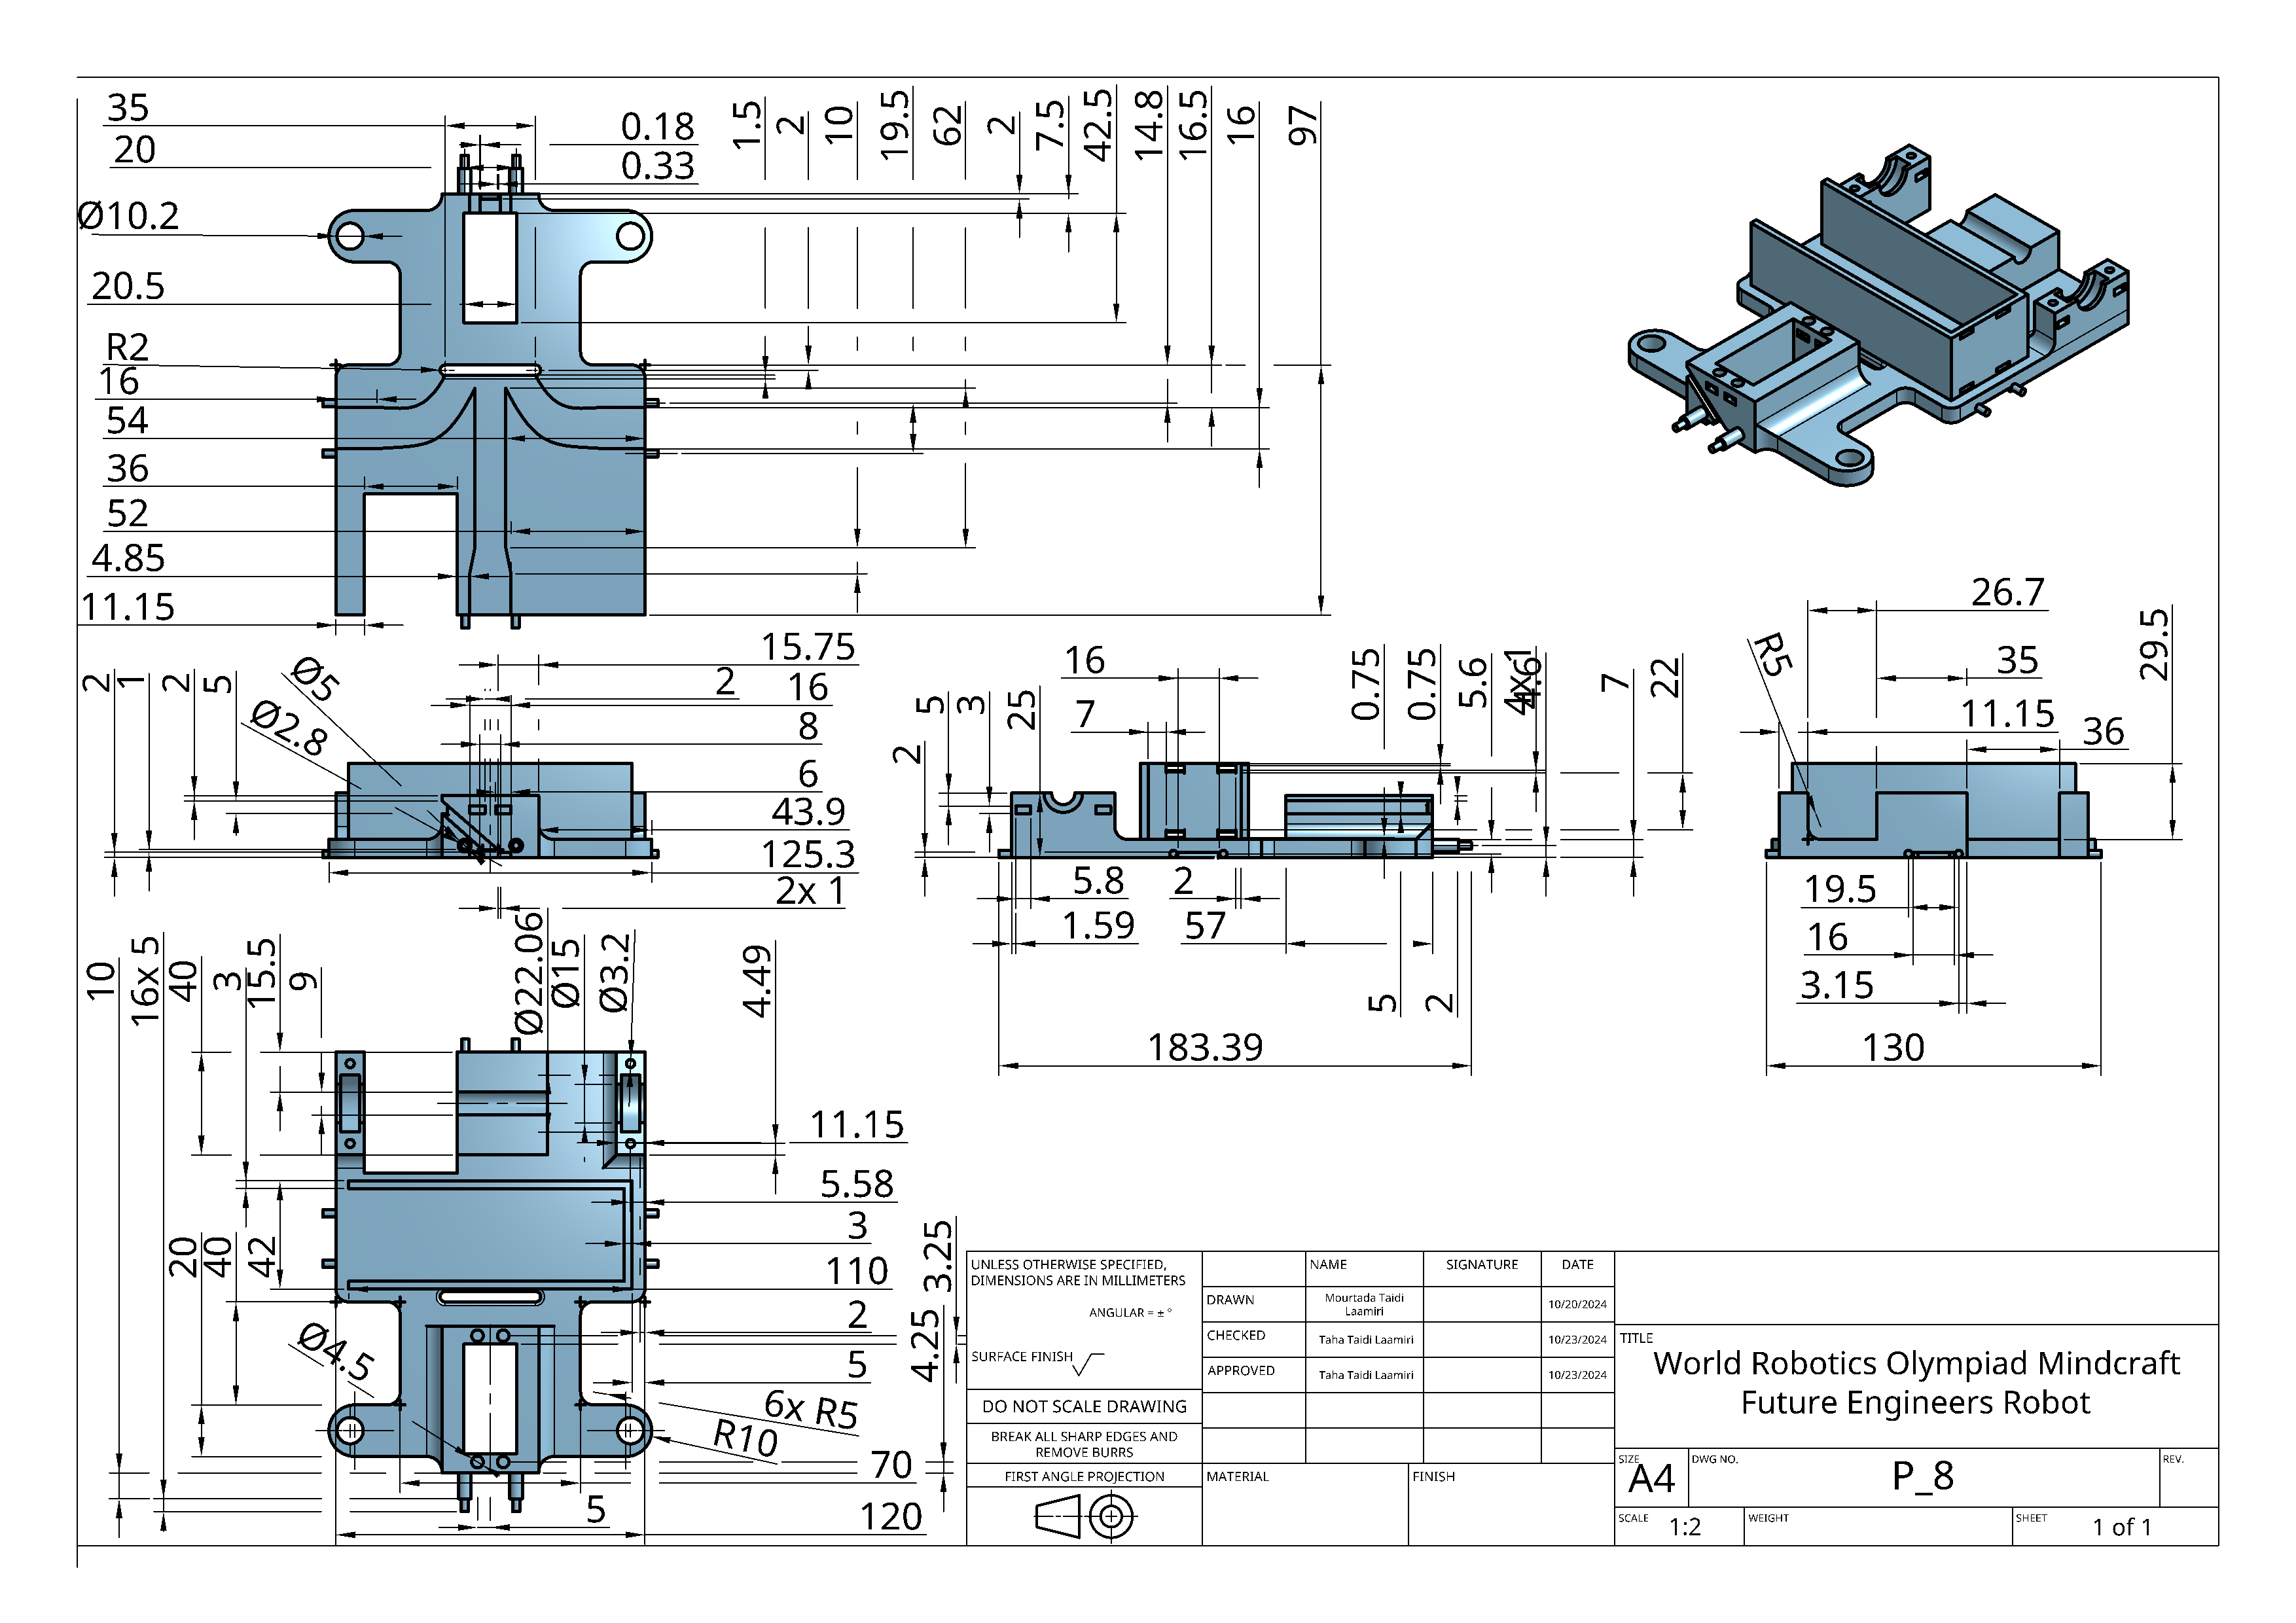
\includegraphics[width=\textwidth, angle=90]{figures/Drawing/Drawing Robot Base.png}
    \caption{Robot Base}
\end{figure}

\begin{figure}[H]
    \vspace{4cm}
    \centering
    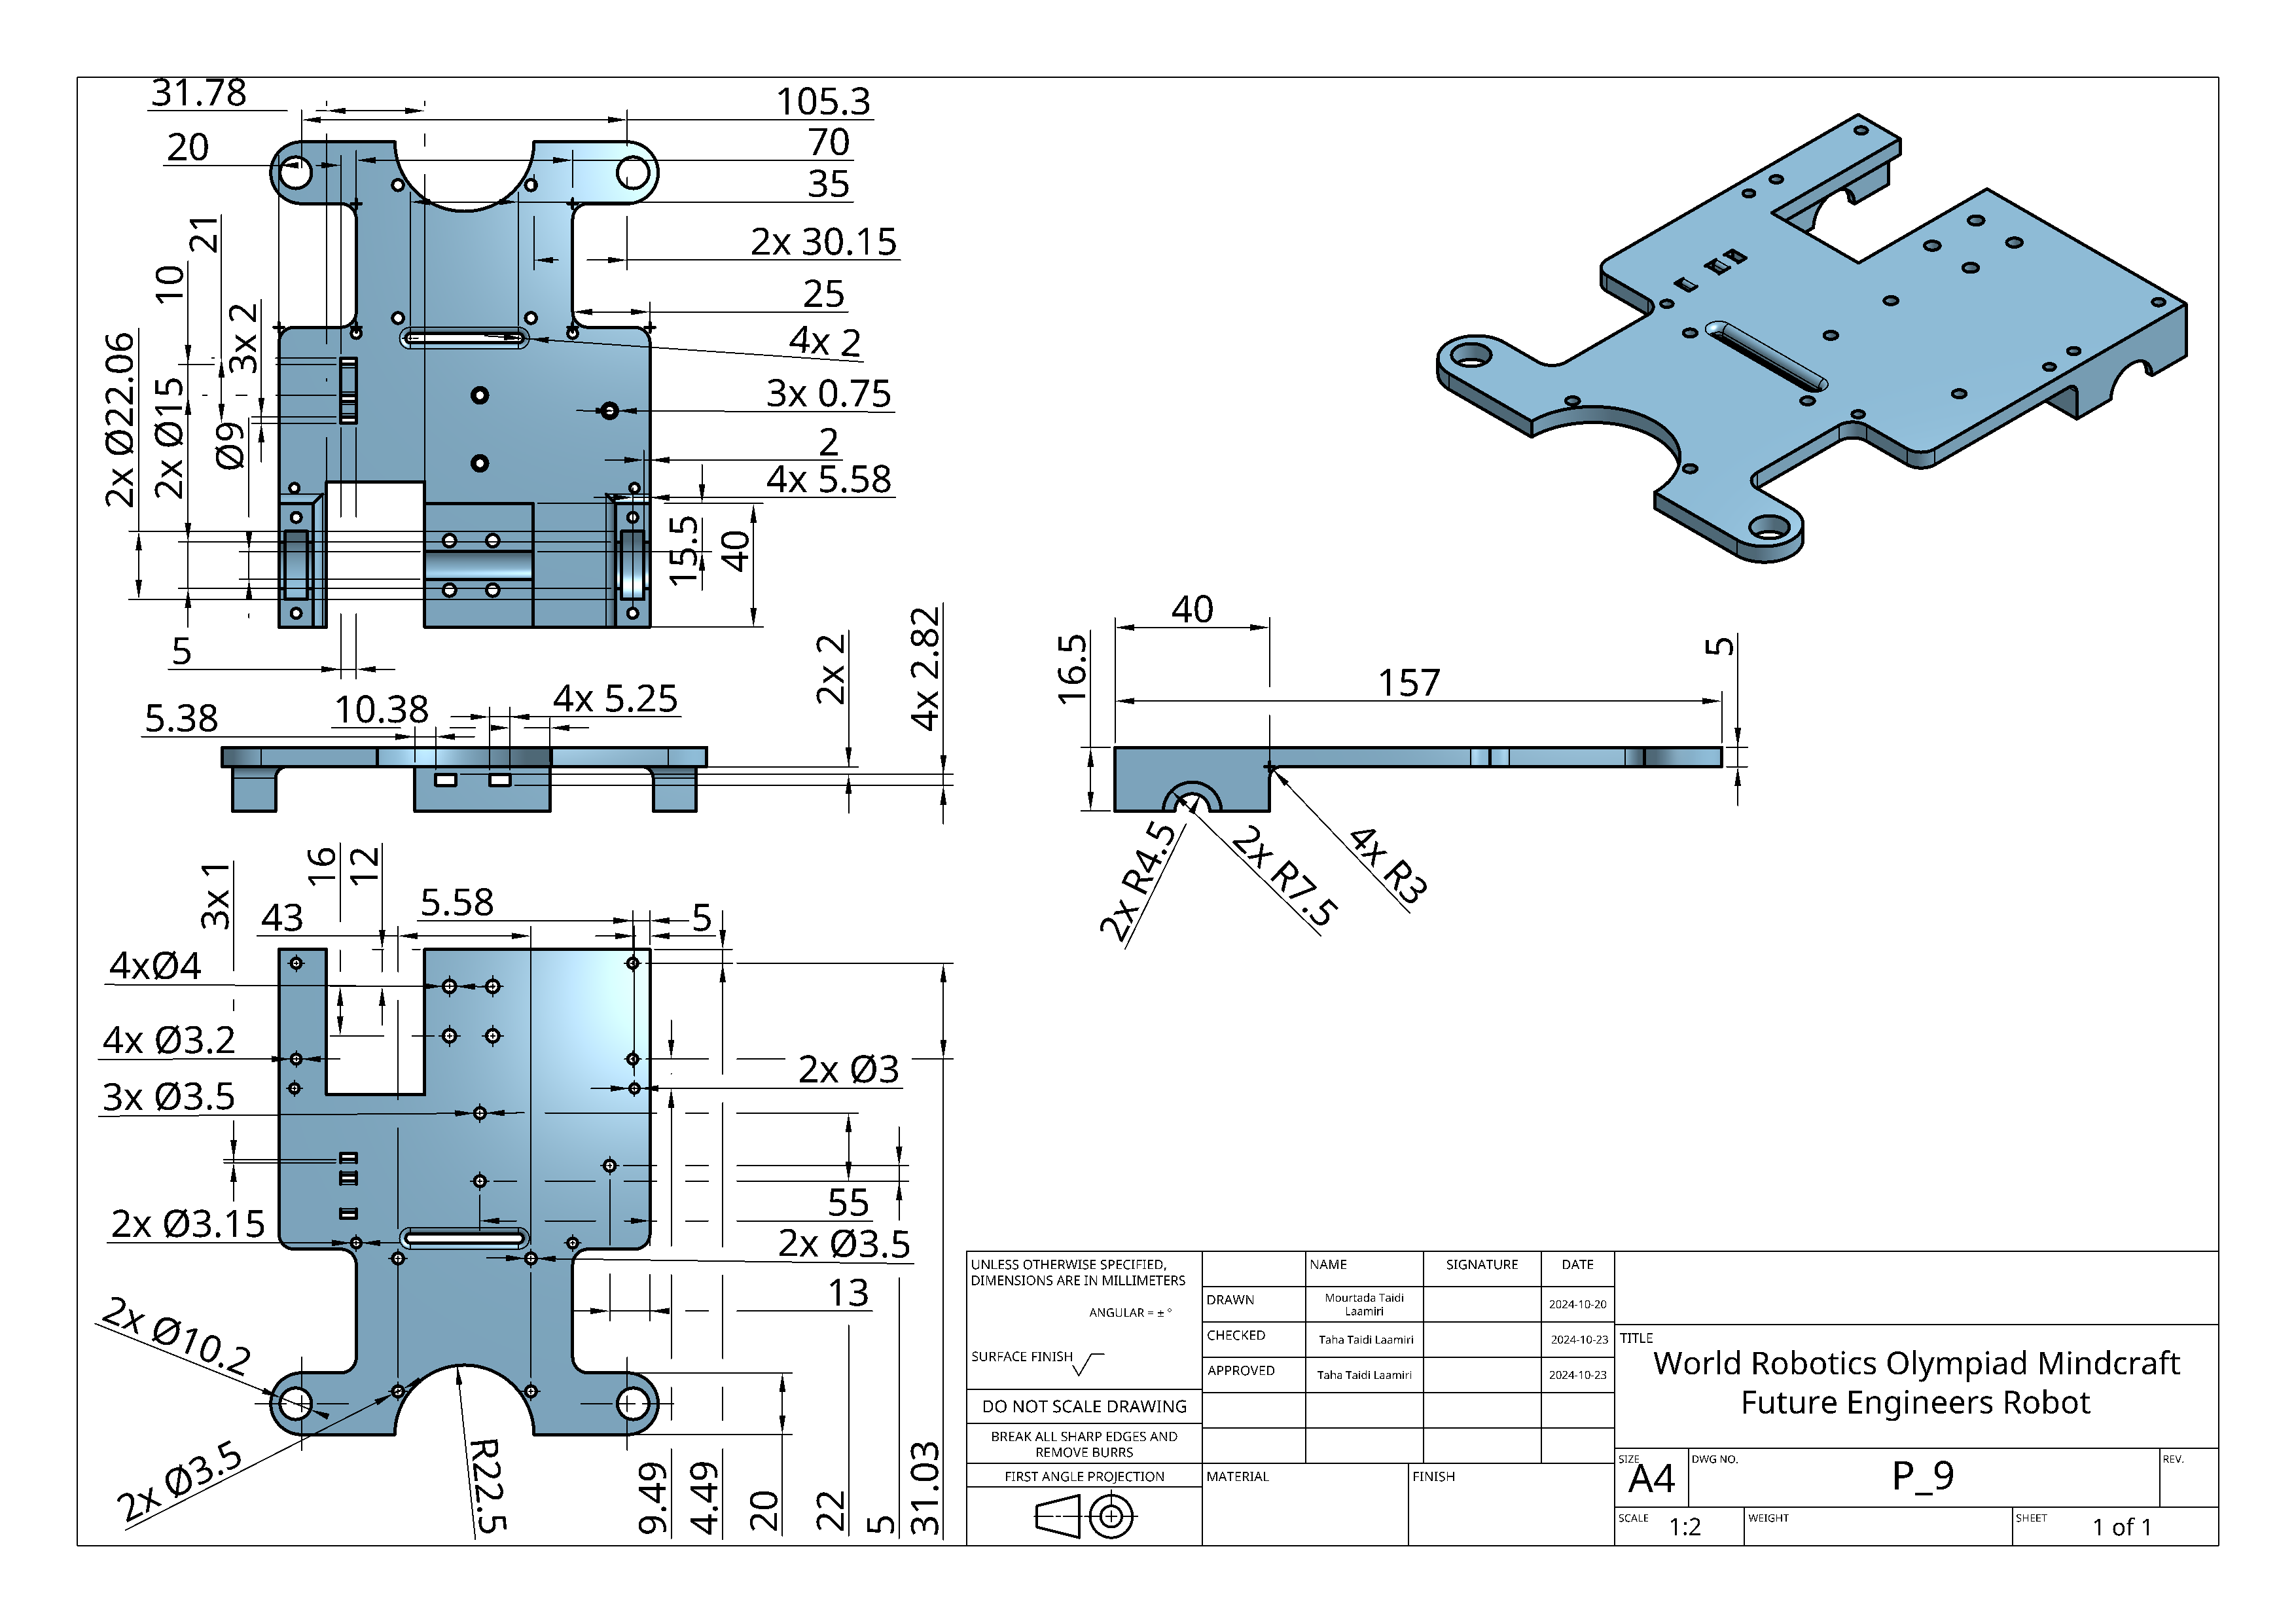
\includegraphics[width=\textwidth, angle=90]{figures/Drawing/Drawing Second Layer.png}
    \caption{Second Layer}
\end{figure}

\begin{figure}[H]
    \vspace{4cm}
    \centering
    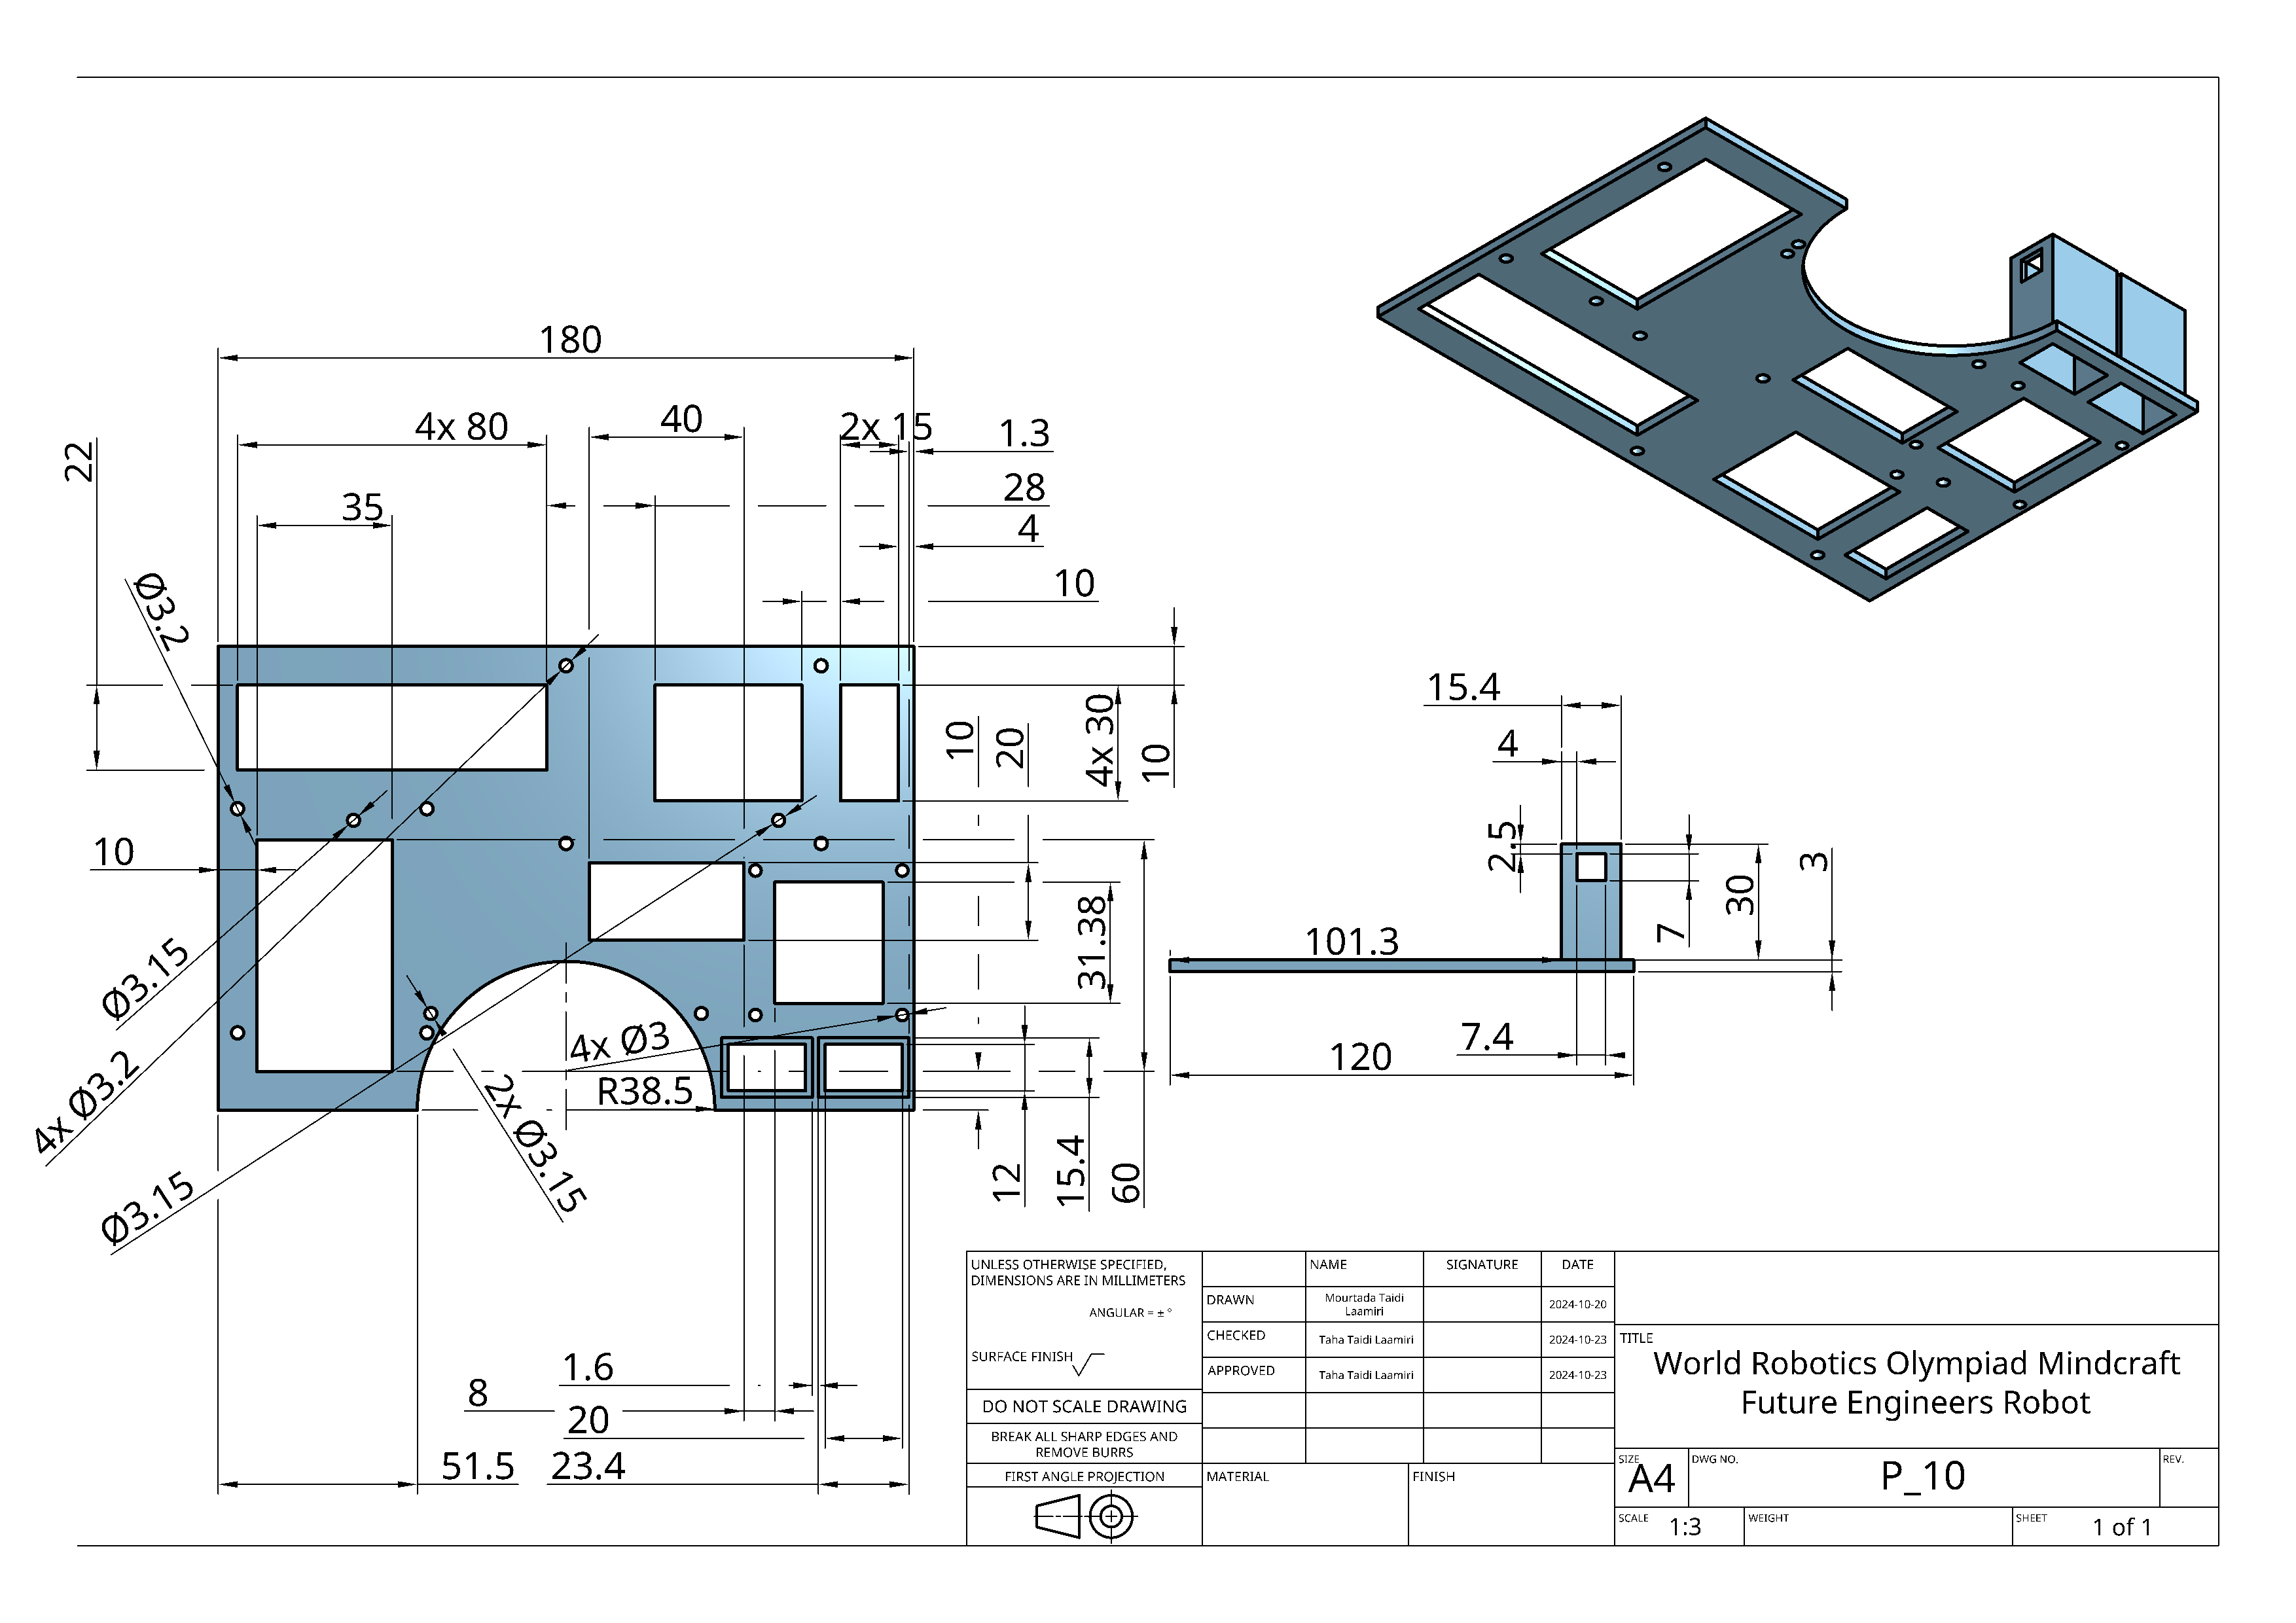
\includegraphics[width=\textwidth, angle=90]{figures/Drawing/Drawing Third Layer.png}
    \caption{Third Layer}
\end{figure}

\begin{figure}[H]
    \vspace{4cm}
    \centering
    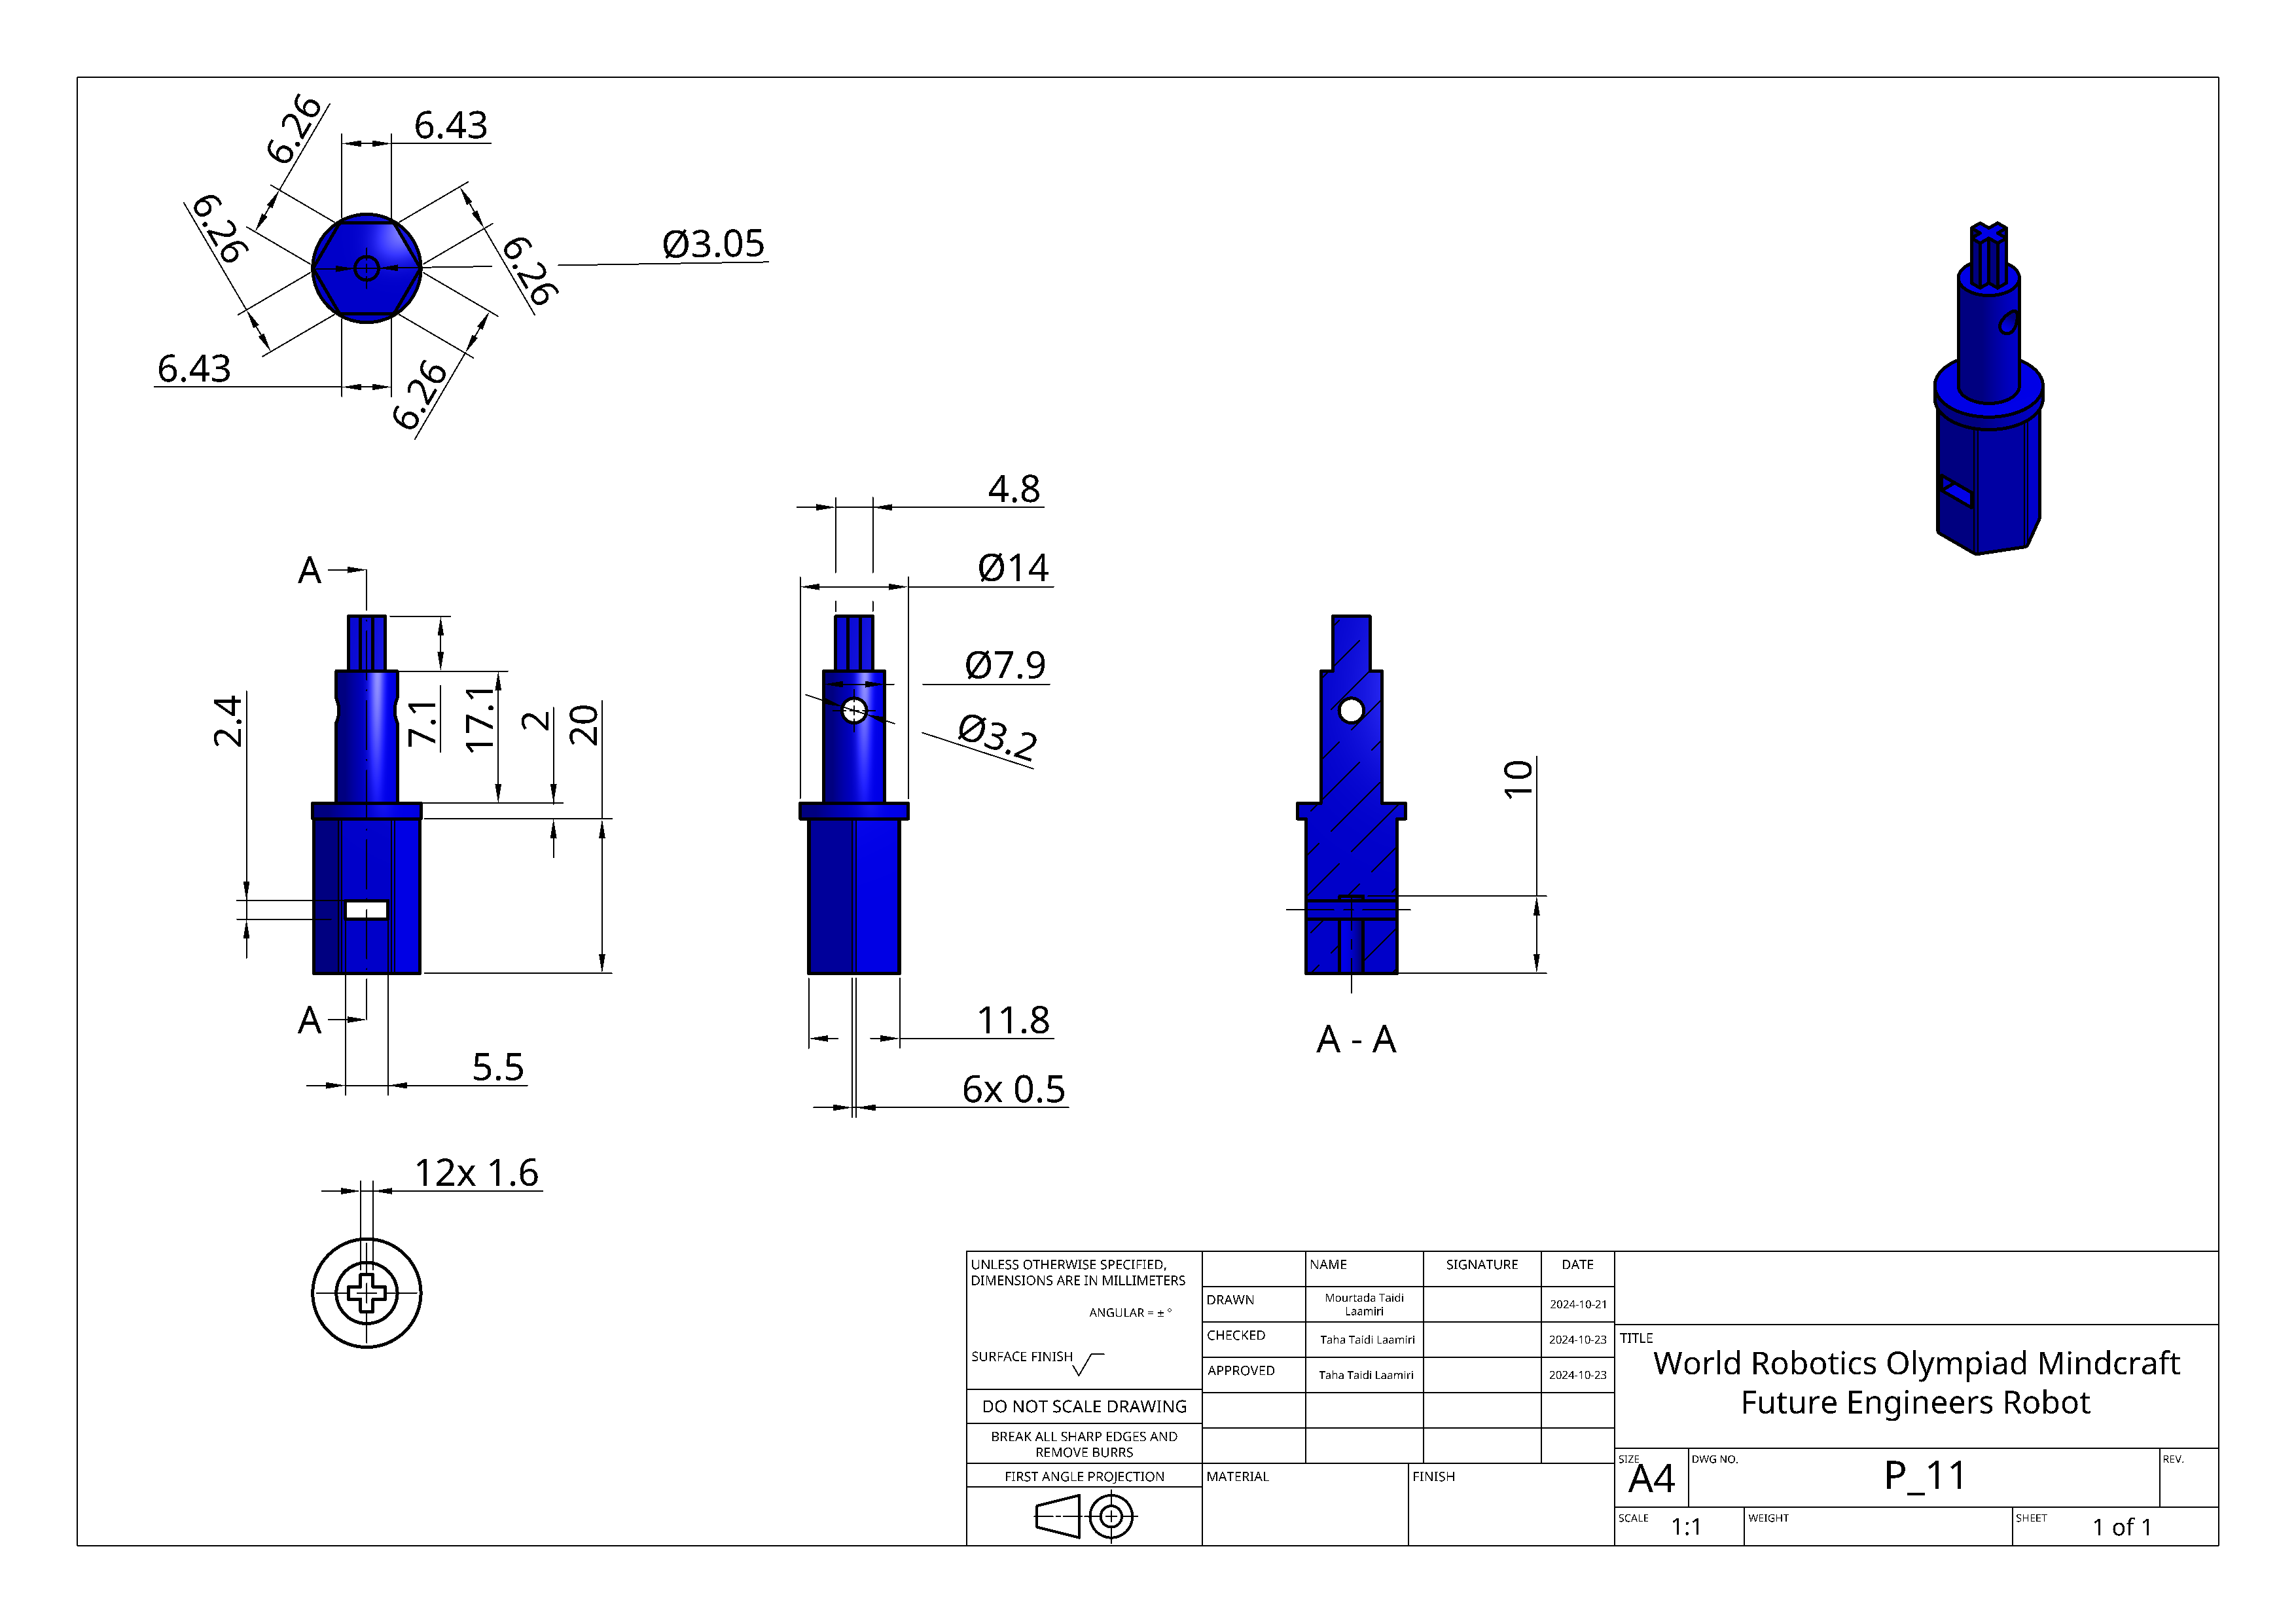
\includegraphics[width=\textwidth, angle=90]{figures/Drawing/Drawing Short Shaft.png}
    \caption{Short Shaft}
\end{figure}

\begin{figure}[H]
    \vspace{4cm}
    \centering
    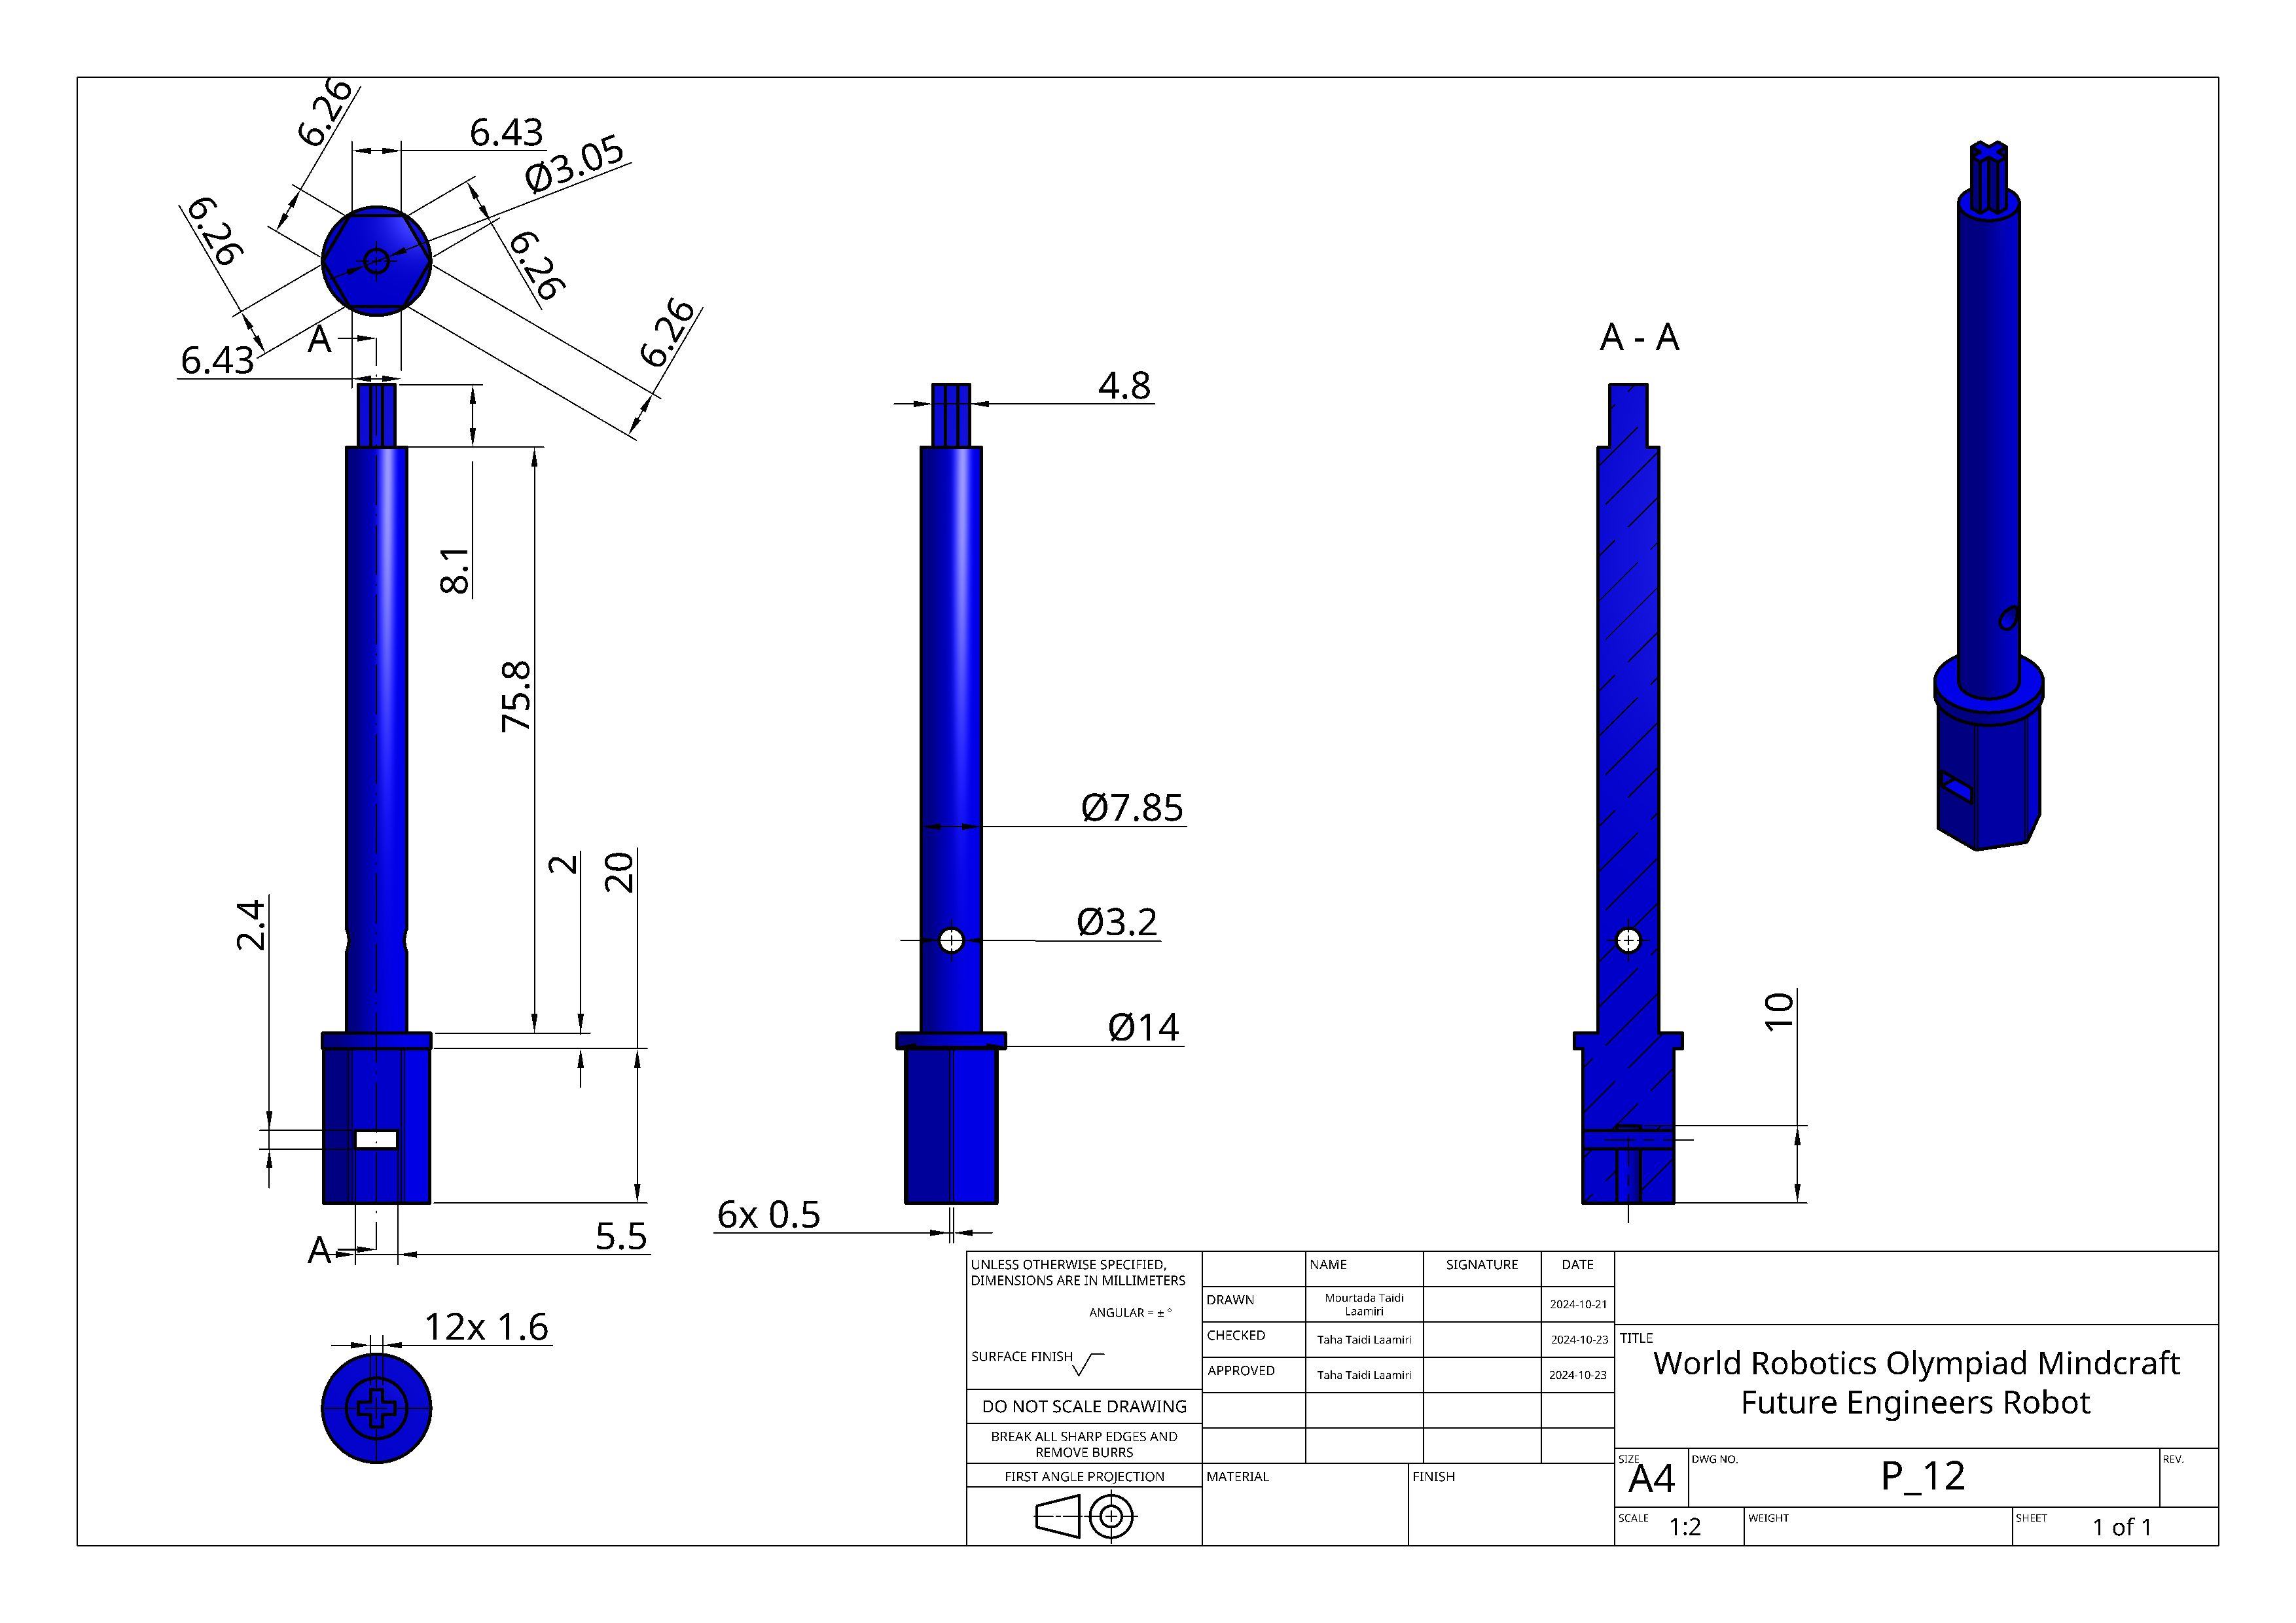
\includegraphics[width=\textwidth, angle=90]{figures/Drawing/Drawing Long Short Shaft.png}
    \caption{Long Shaft}
\end{figure}

\begin{figure}[H]
    \vspace{4cm}
    \centering
    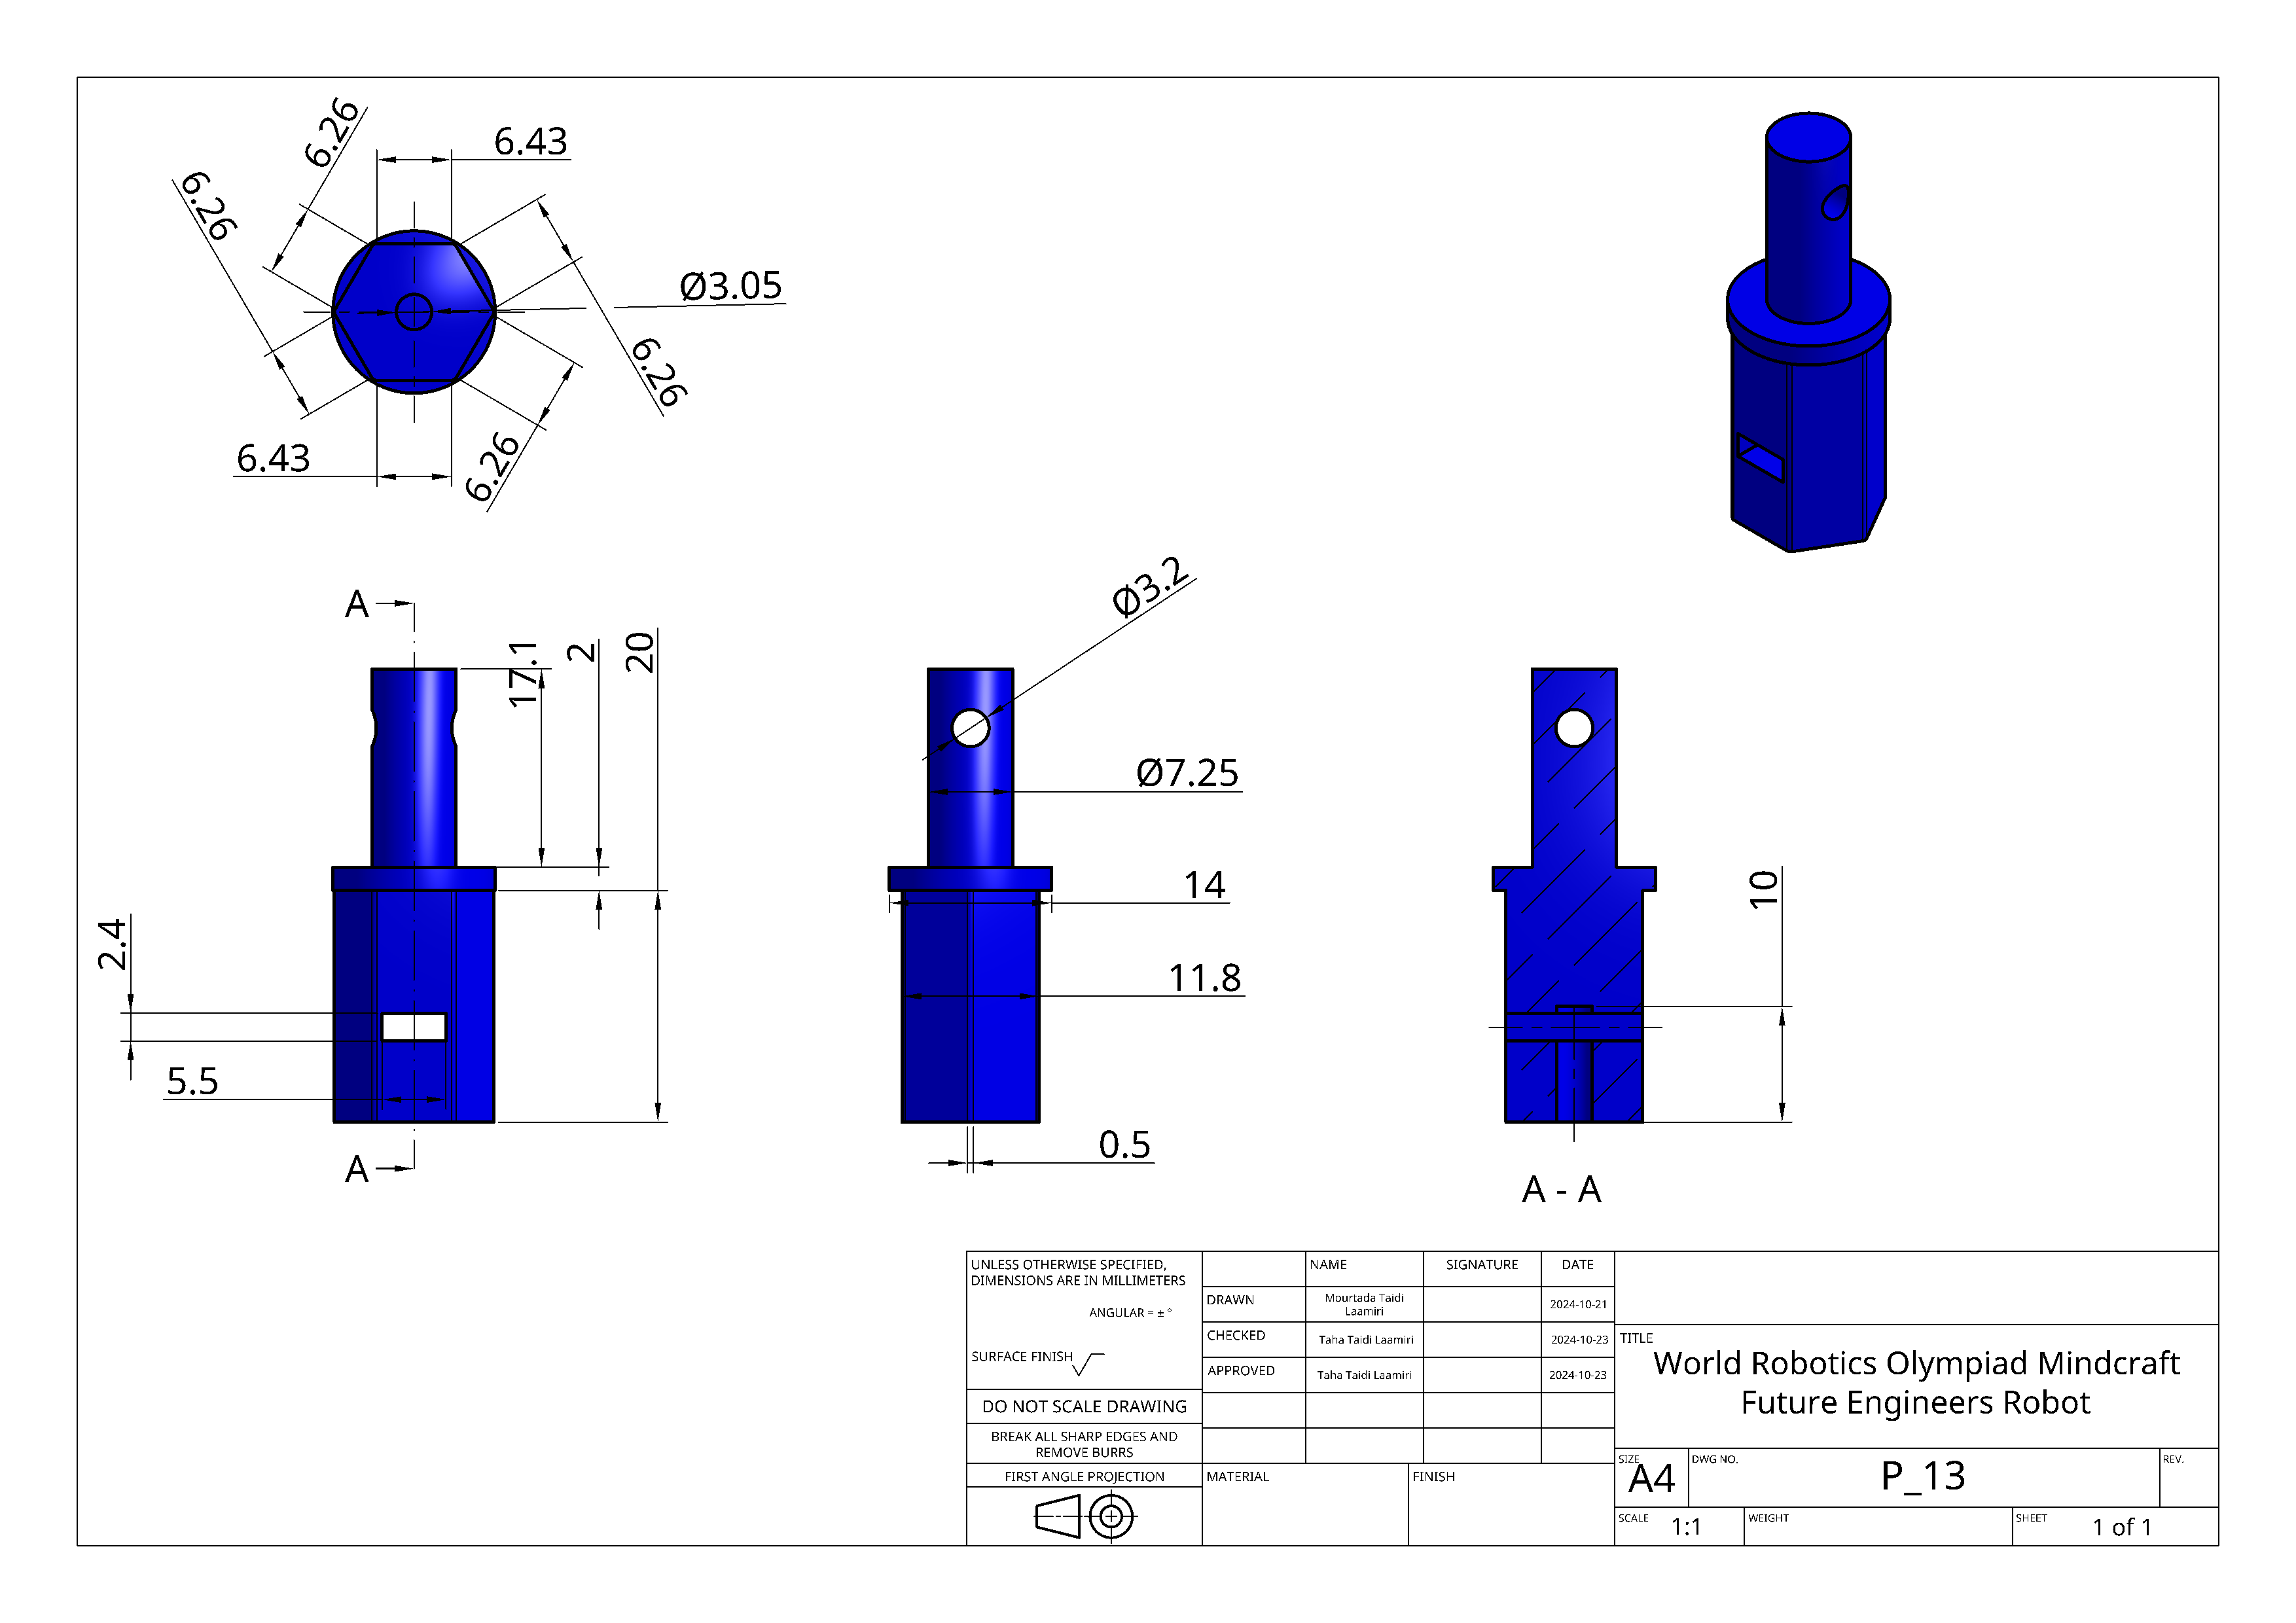
\includegraphics[width=\textwidth, angle=90]{figures/Drawing/Drawing Front Short Shaft.png}
    \caption{Front Short Shaft}
\end{figure}

\begin{figure}[H]
    \vspace{4cm}
    \centering
    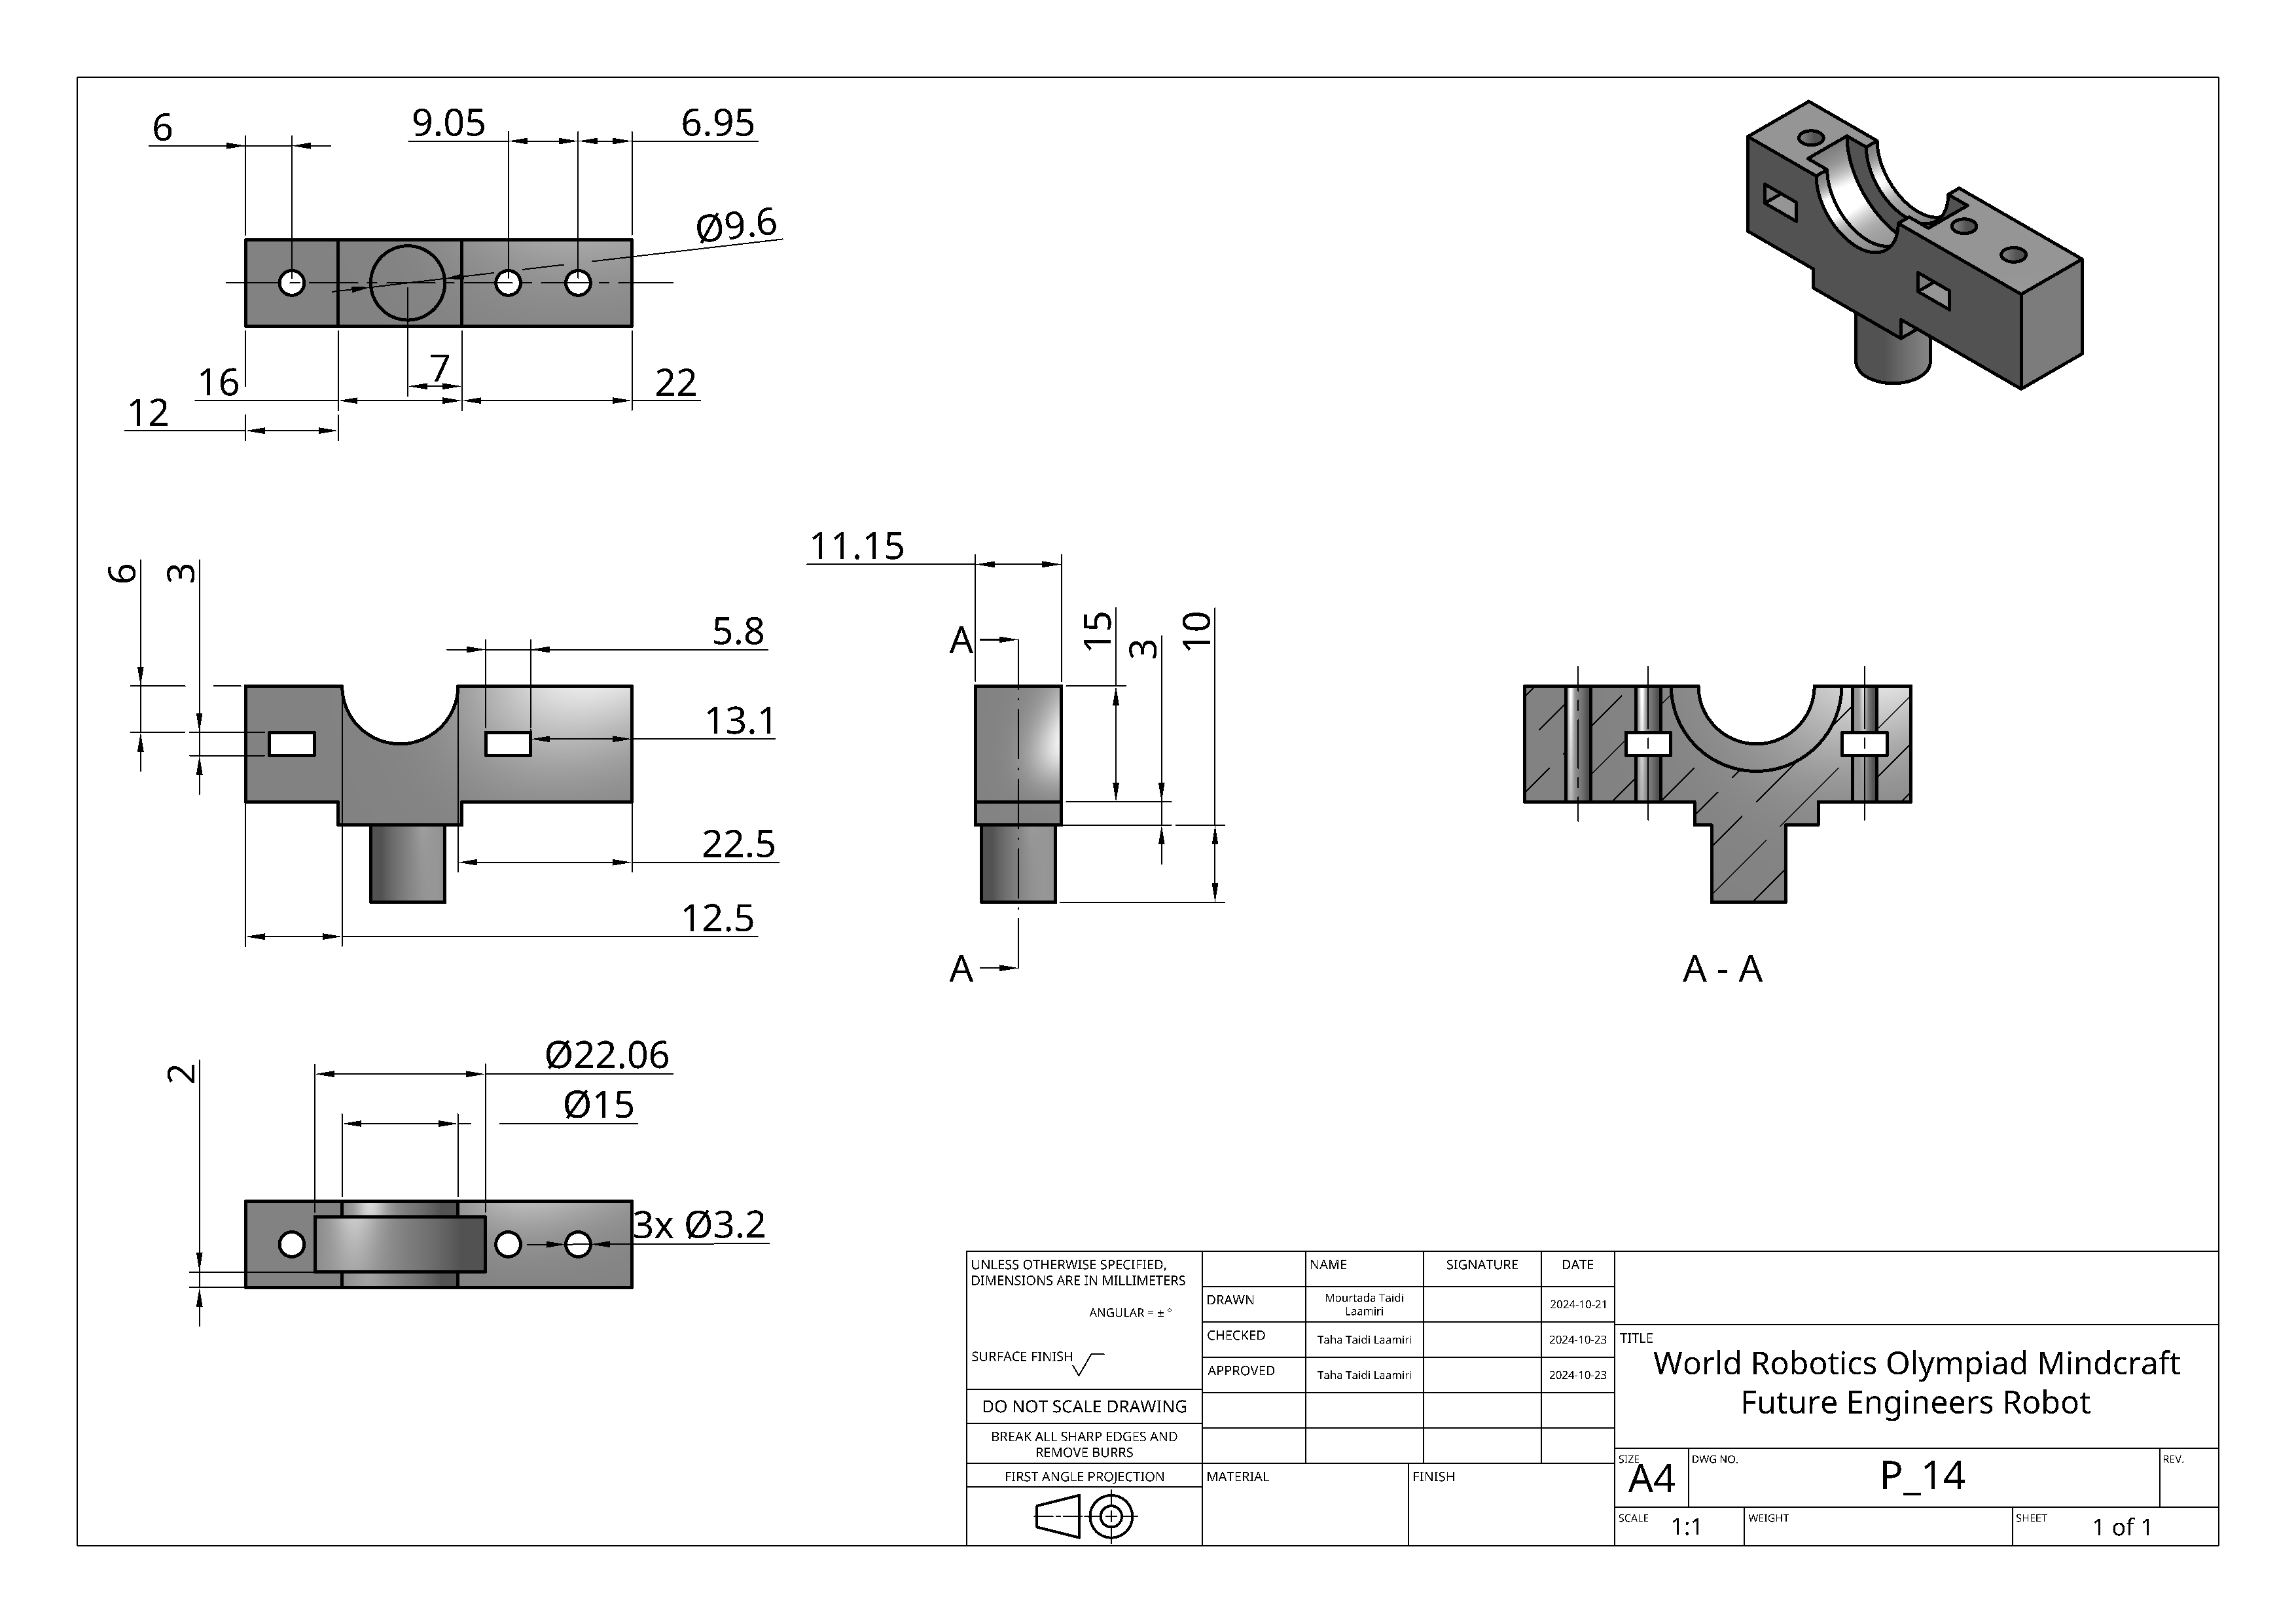
\includegraphics[width=\textwidth, angle=90]{figures/Drawing/Drawing Support Front Bottom.png}
    \caption{Berring Support Front Bottom}
\end{figure}

\begin{figure}[H]
    \vspace{4cm}
    \centering
    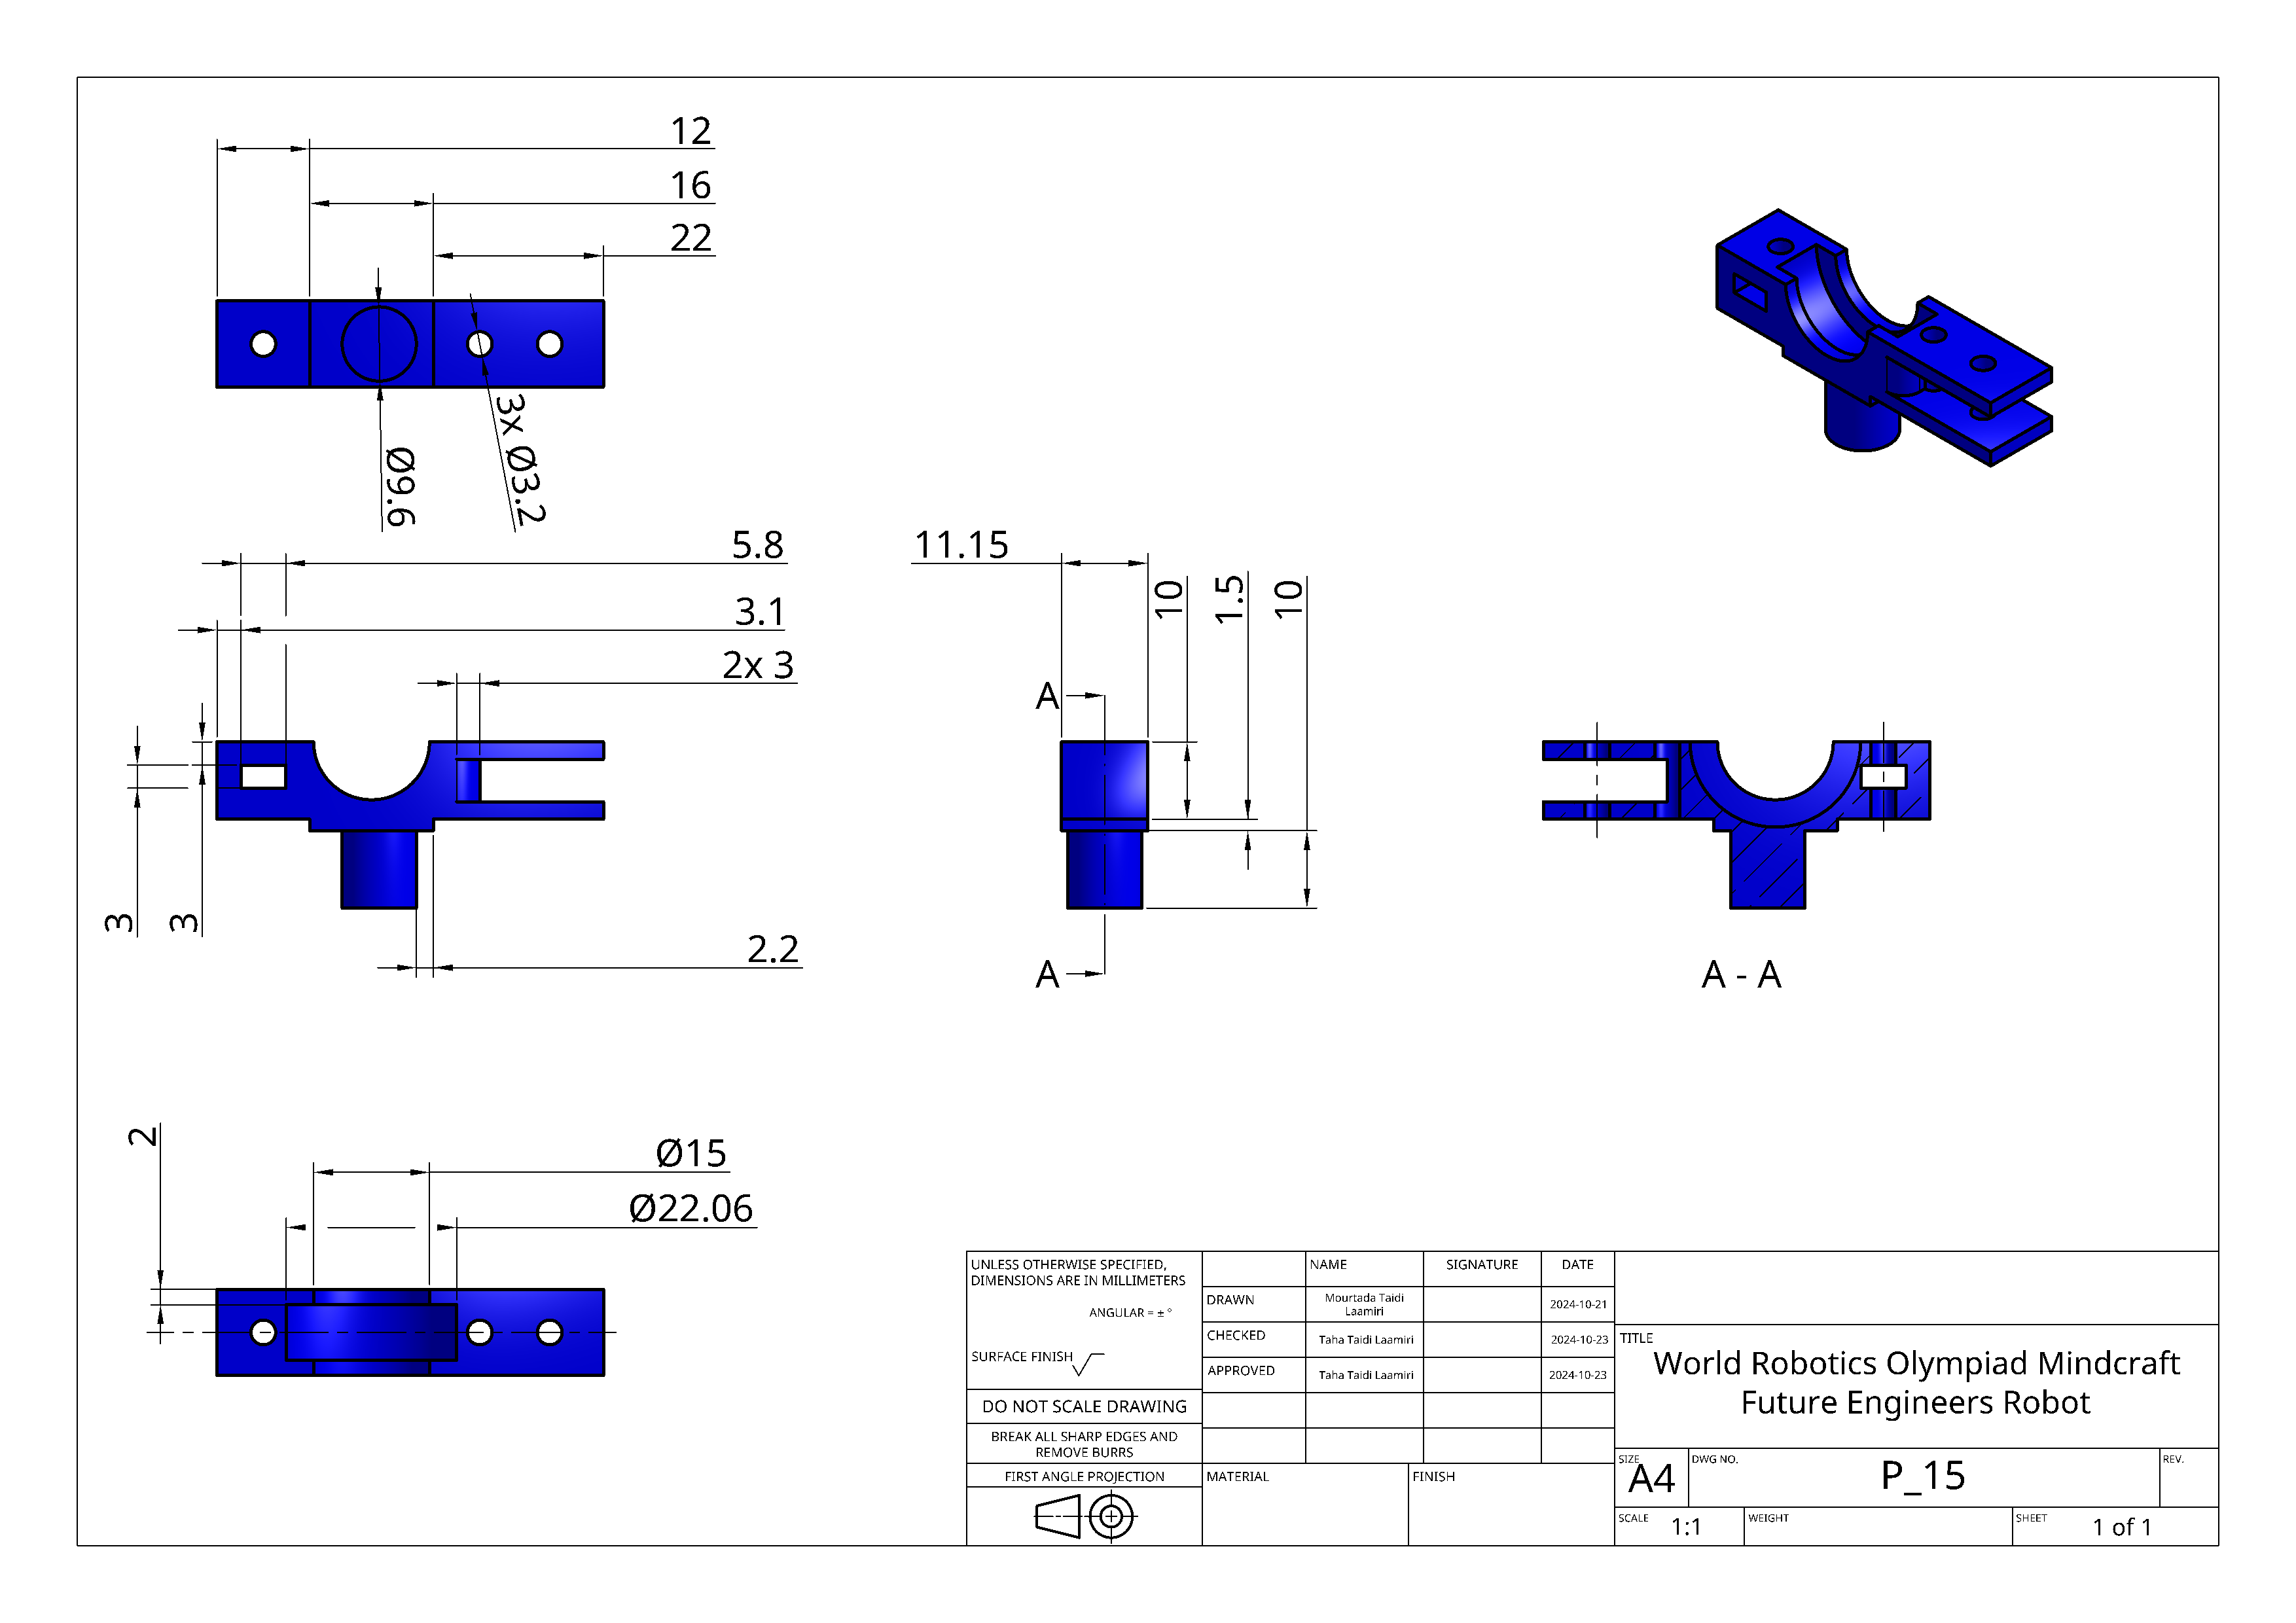
\includegraphics[width=\textwidth, angle=90]{figures/Drawing/Drawing Berring Front Top.png}
    \caption{Berring Support Front Top}
\end{figure}

\begin{figure}[H]
    \vspace{4cm}
    \centering
    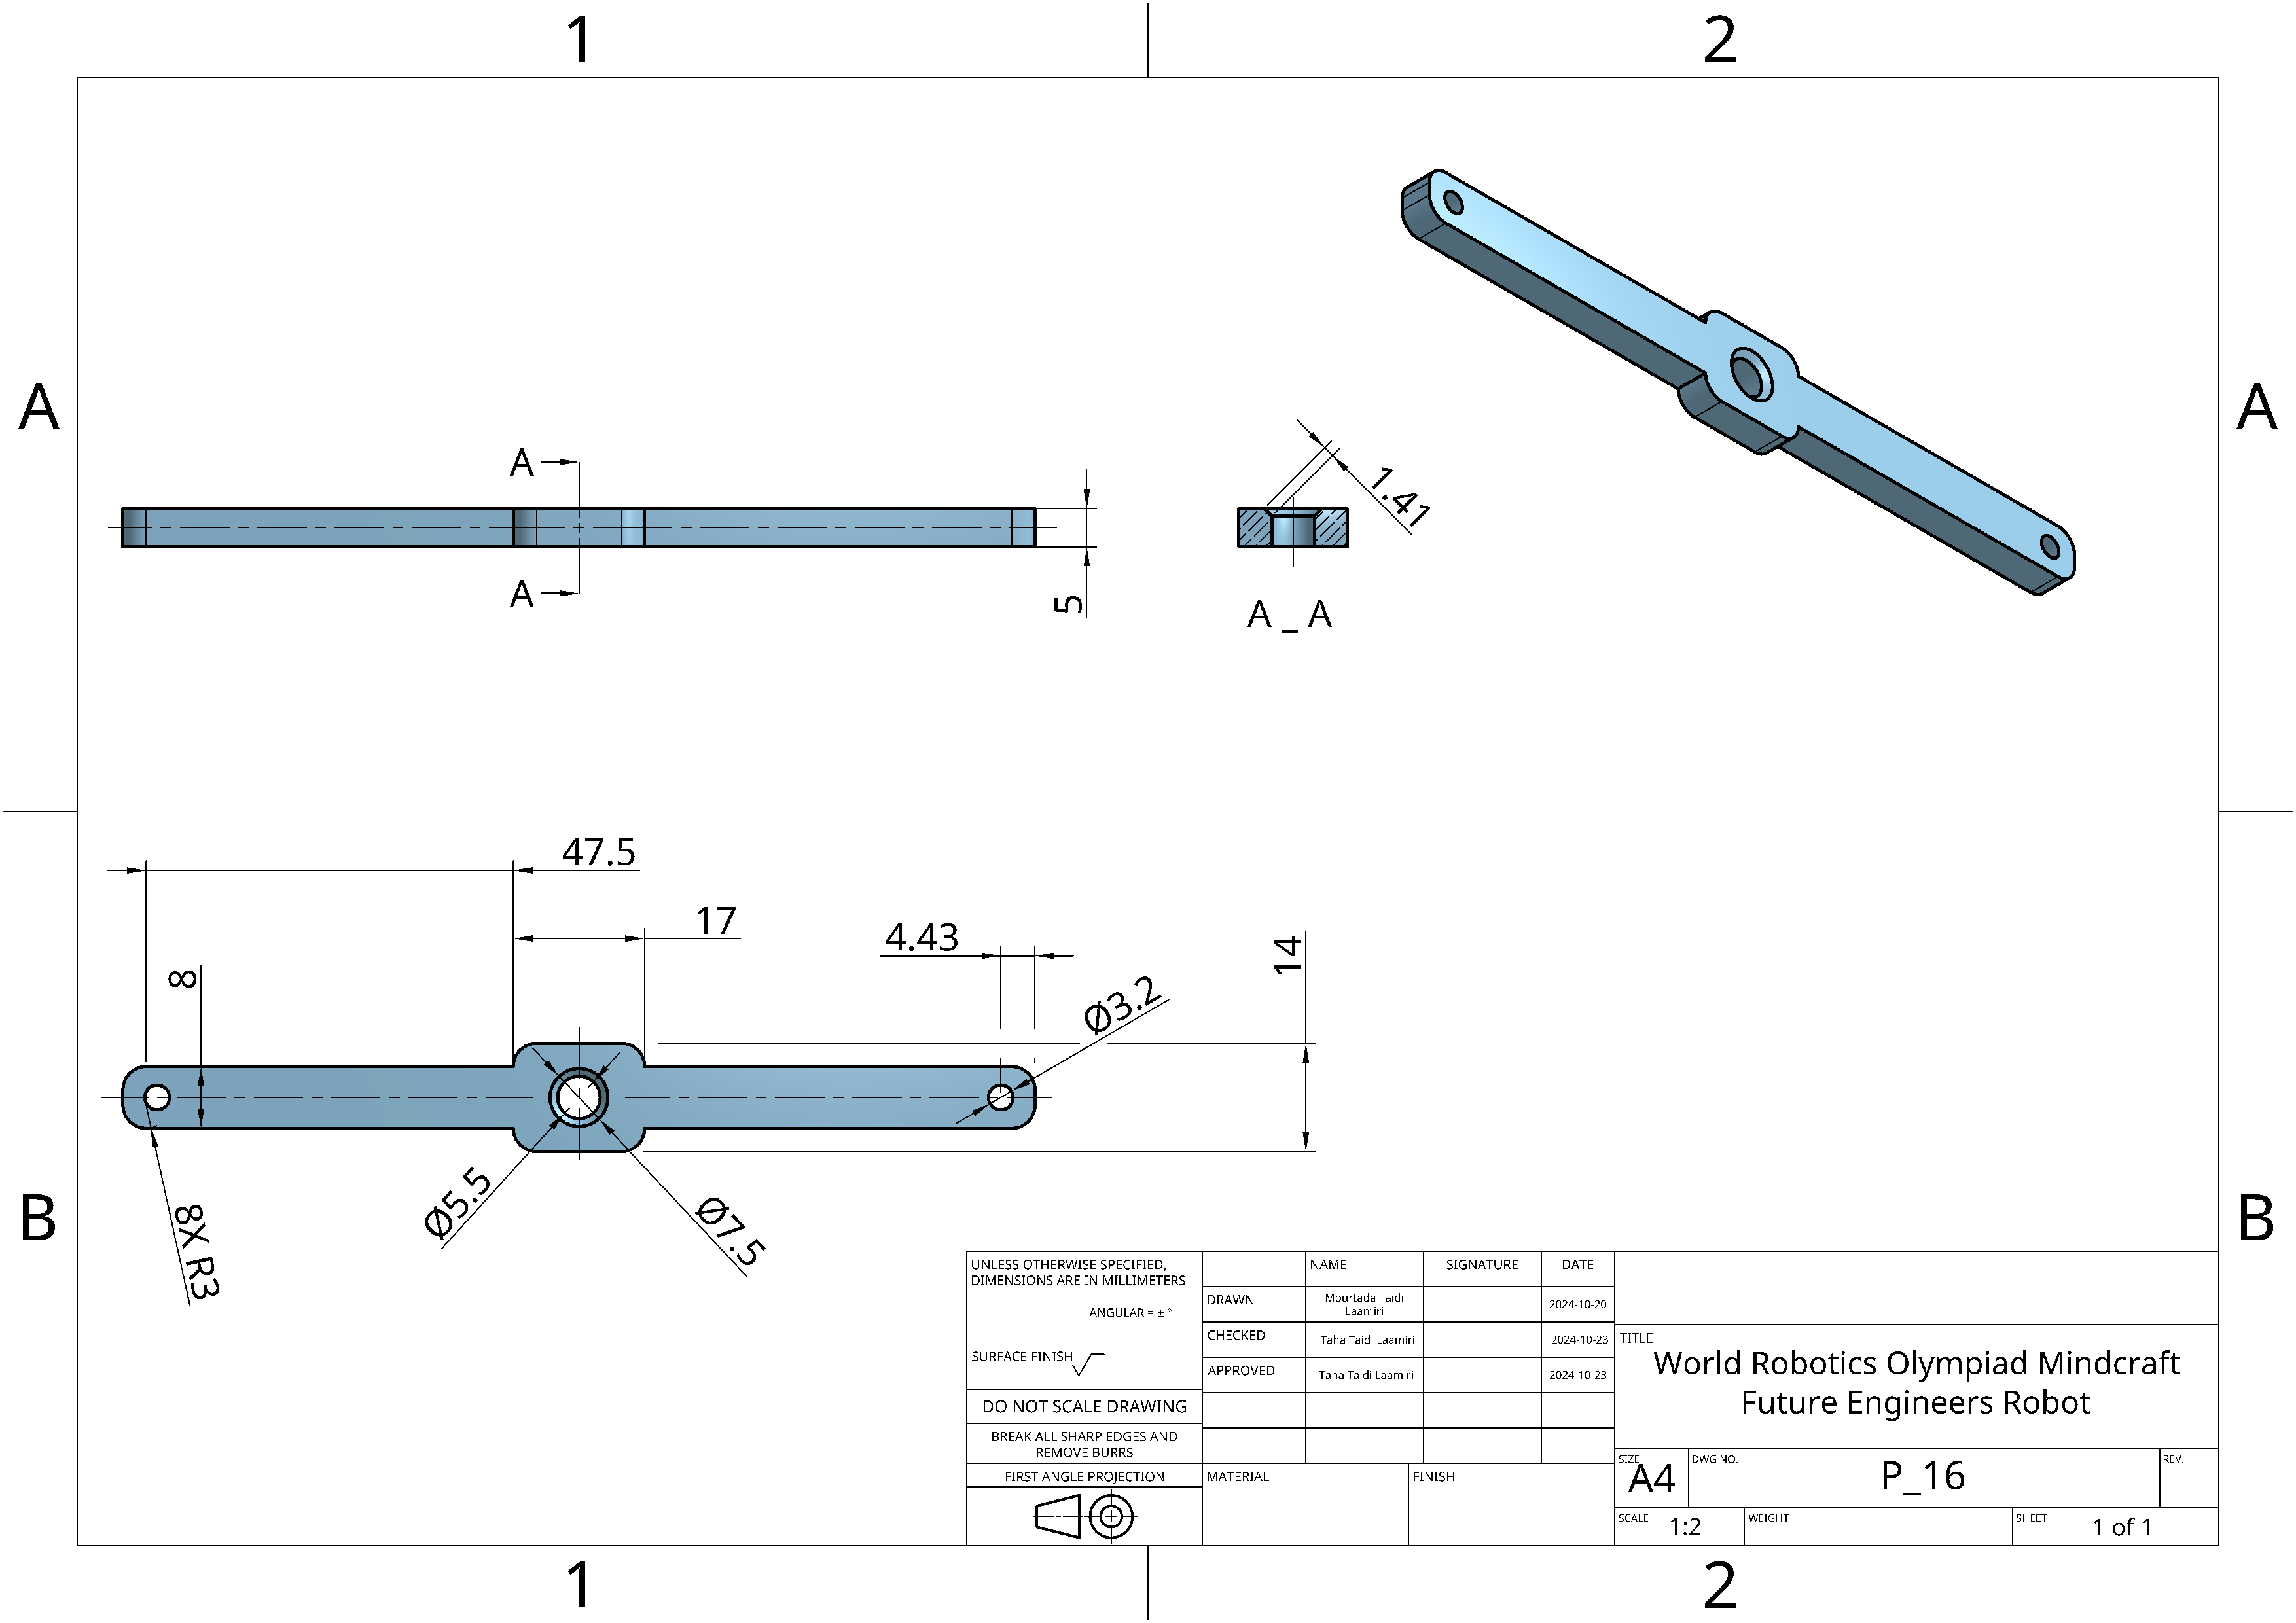
\includegraphics[width=\textwidth, angle=90]{figures/Drawing/Drawing Steering Rack.png}
    \caption{Steering Rack}
\end{figure}

\begin{figure}[H]
    \vspace{4cm}
    \centering
    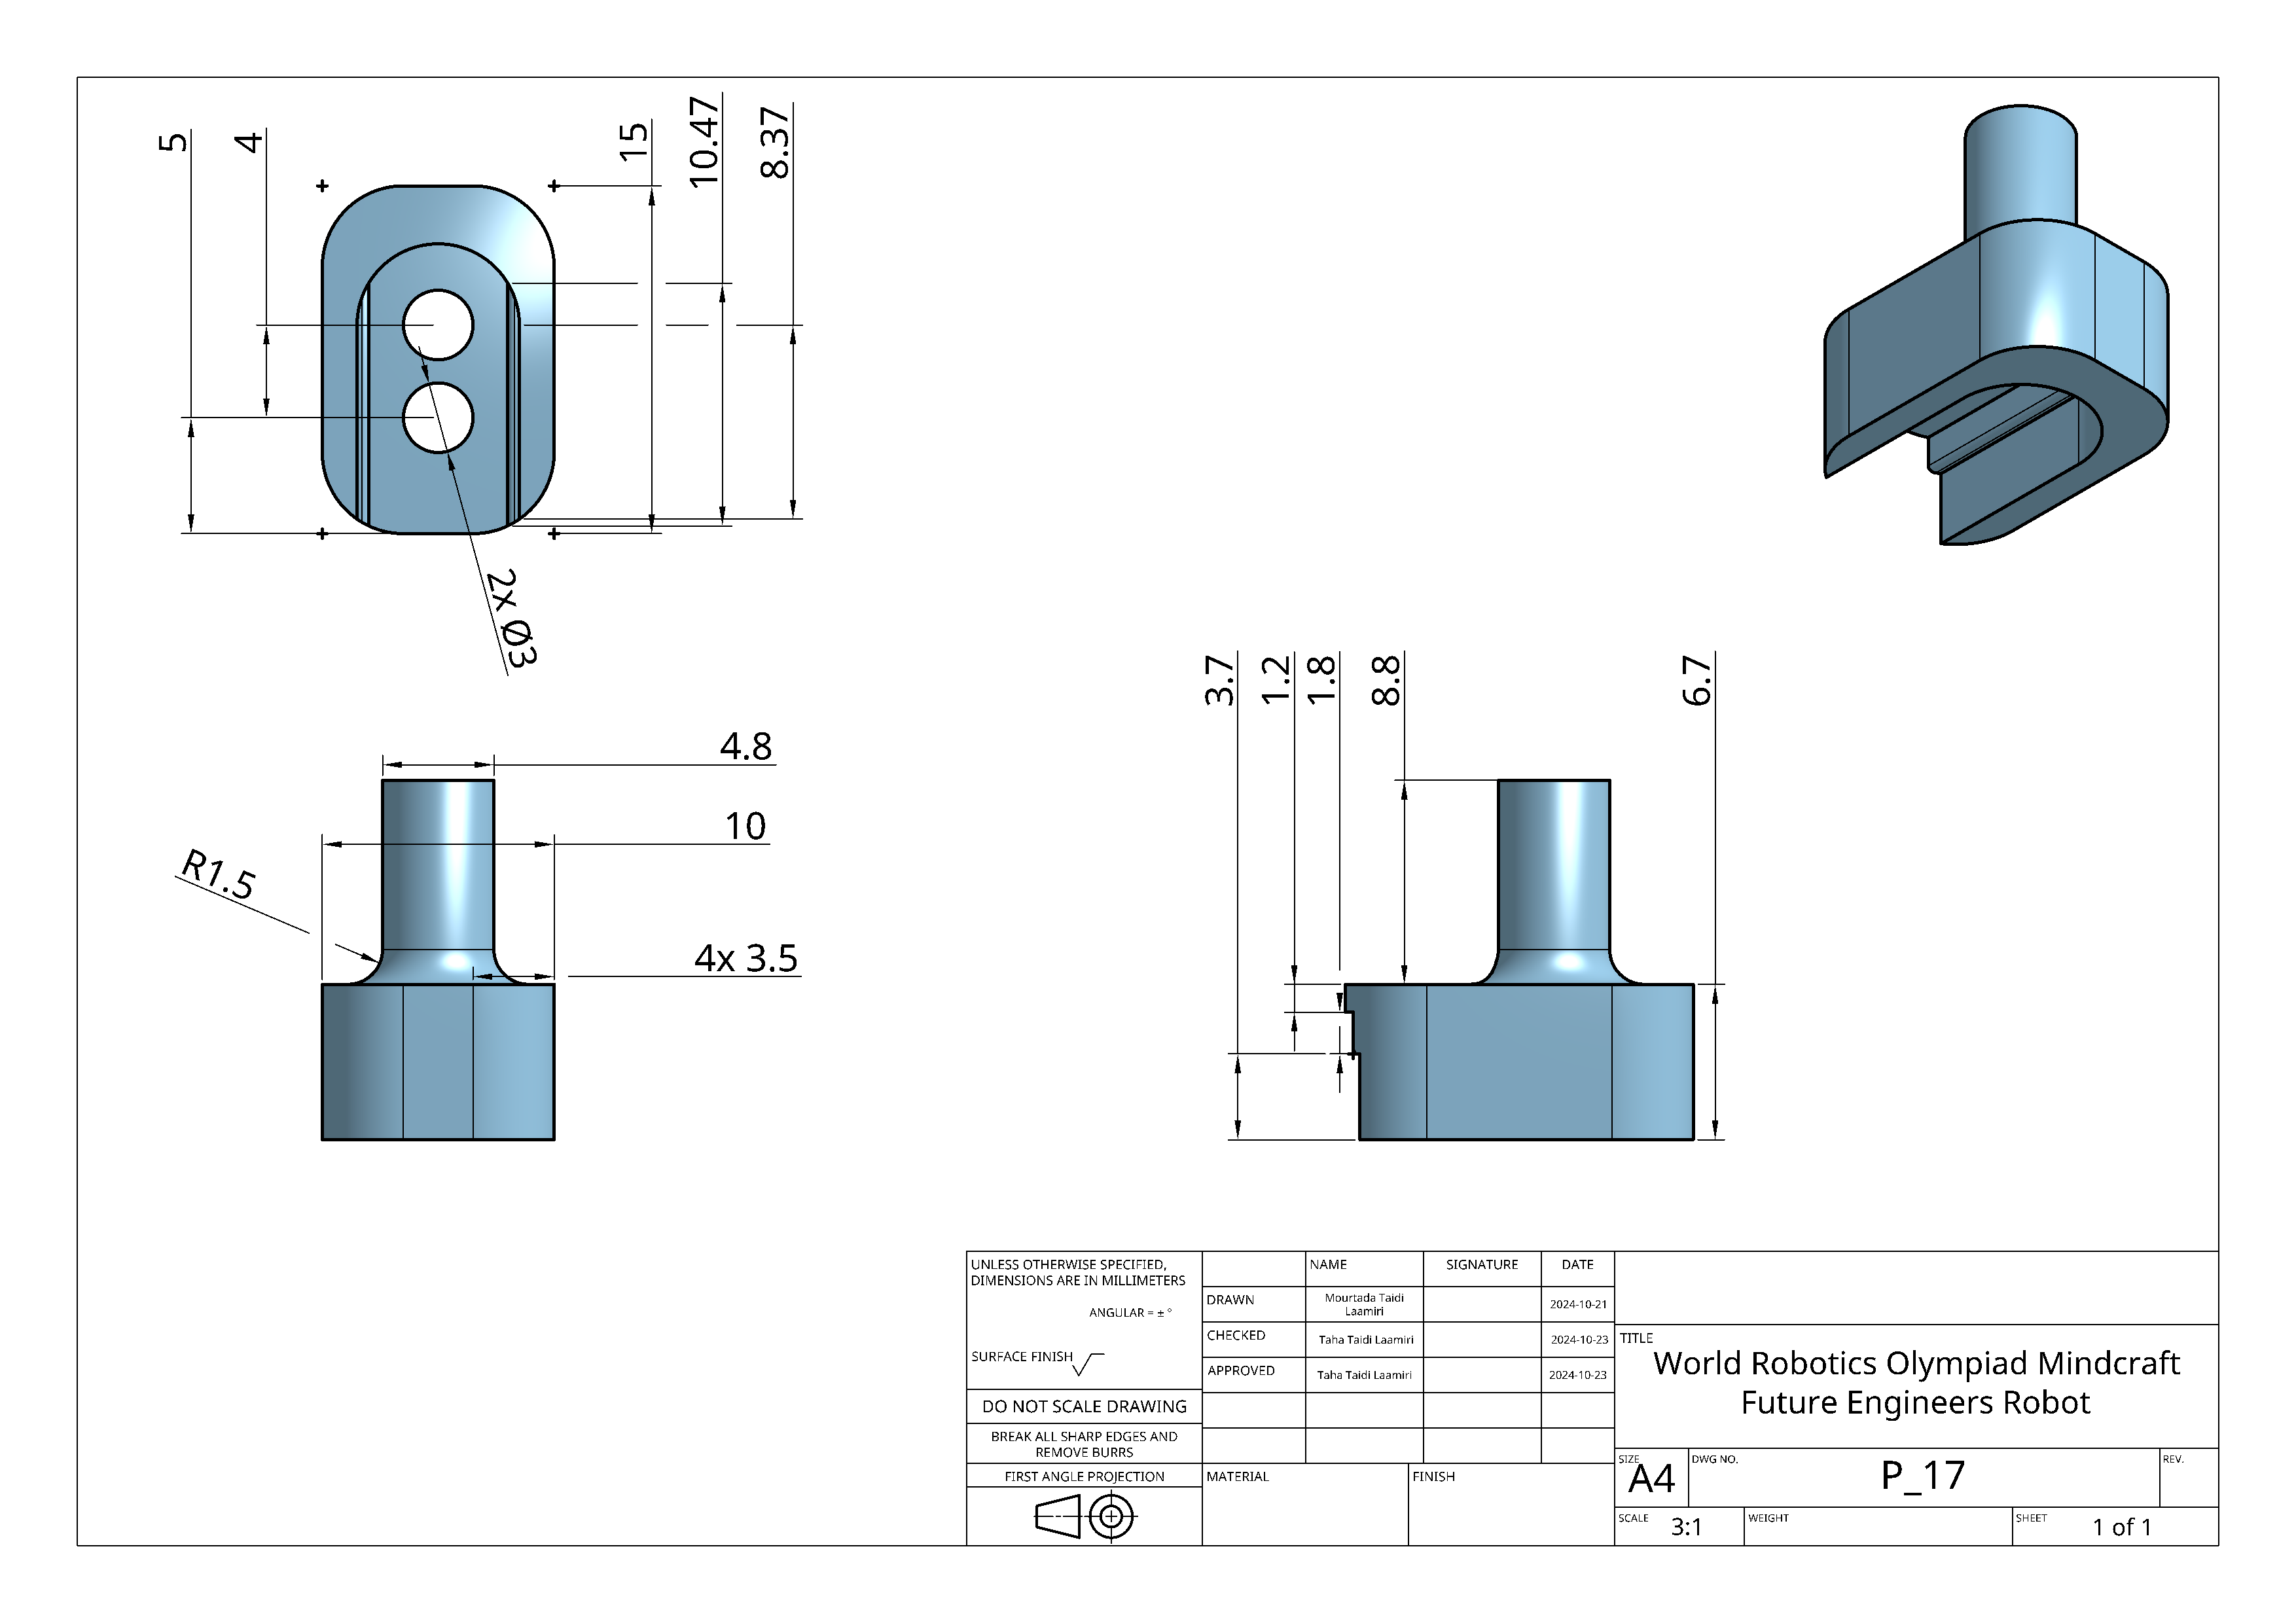
\includegraphics[width=\textwidth, angle=90]{figures/Drawing/Drawing Steering Conector.png}
    \caption{Steering Conector}
\end{figure}

\begin{figure}[H]
    \vspace{4cm}
    \centering
    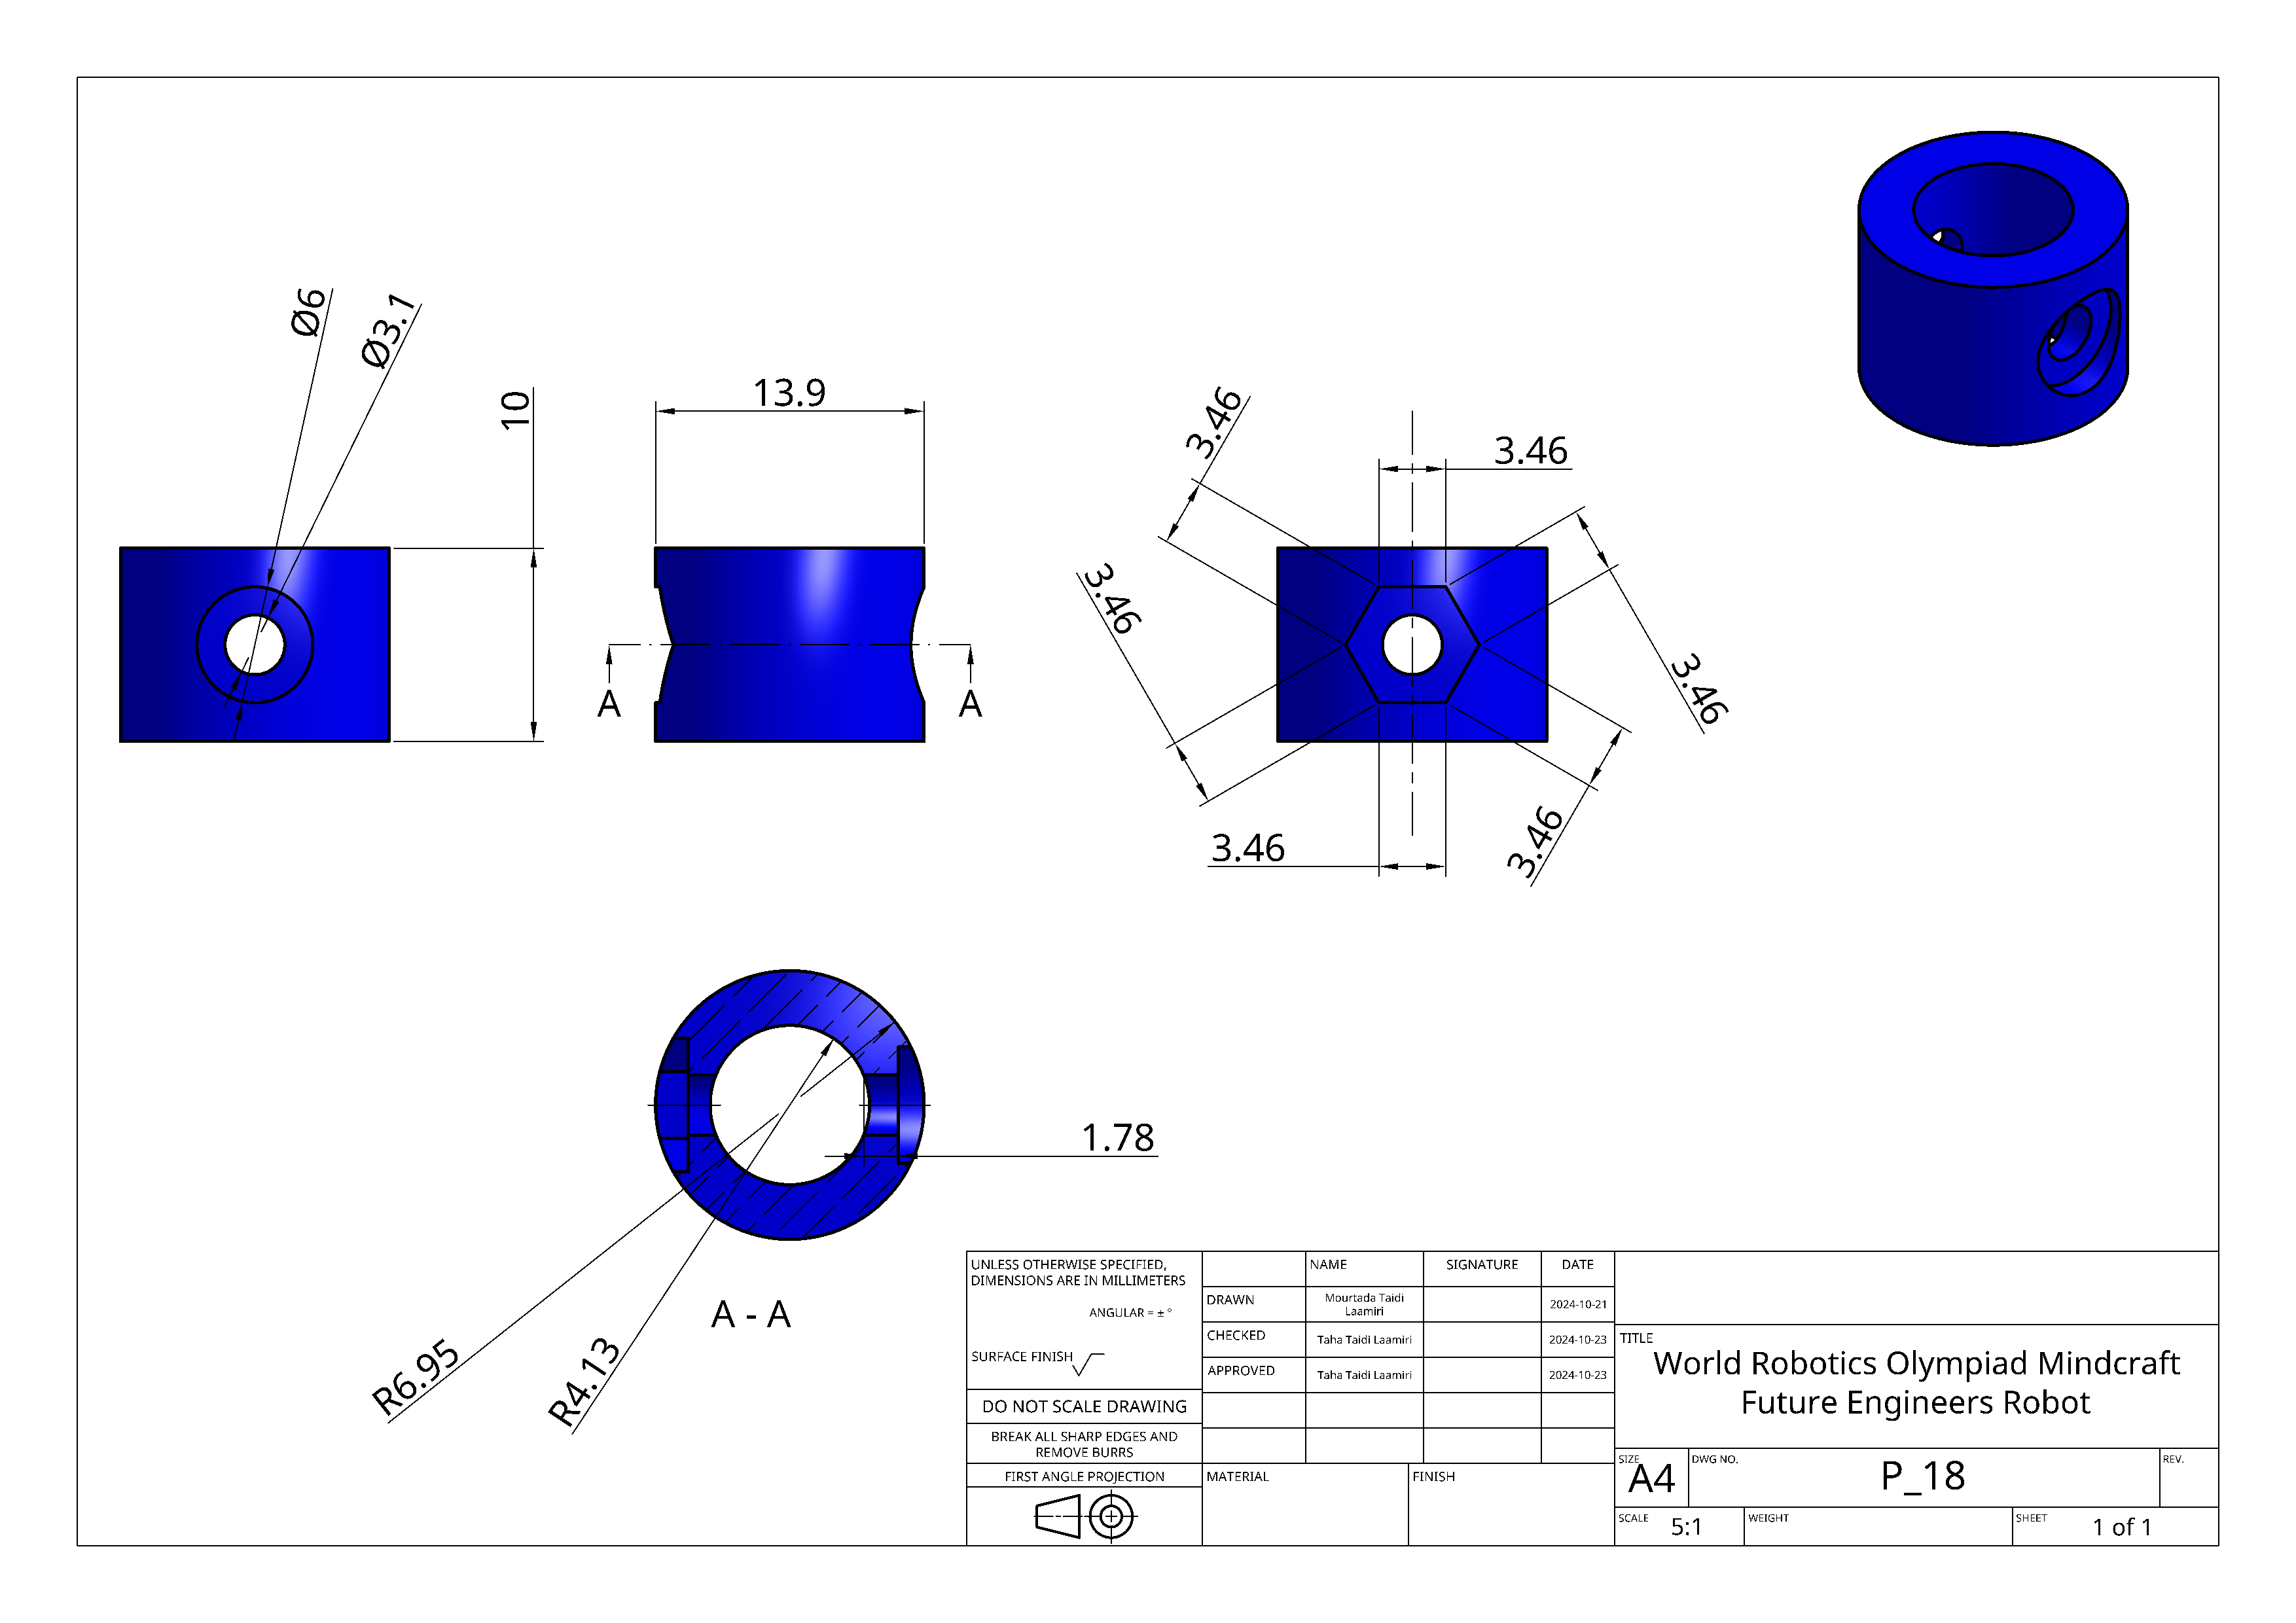
\includegraphics[width=\textwidth, angle=90]{figures/Drawing/Drawing Axle Calamp.png}
    \caption{Axle Clamp}
\end{figure}

\begin{figure}[H]
    \vspace{4cm}
    \centering
    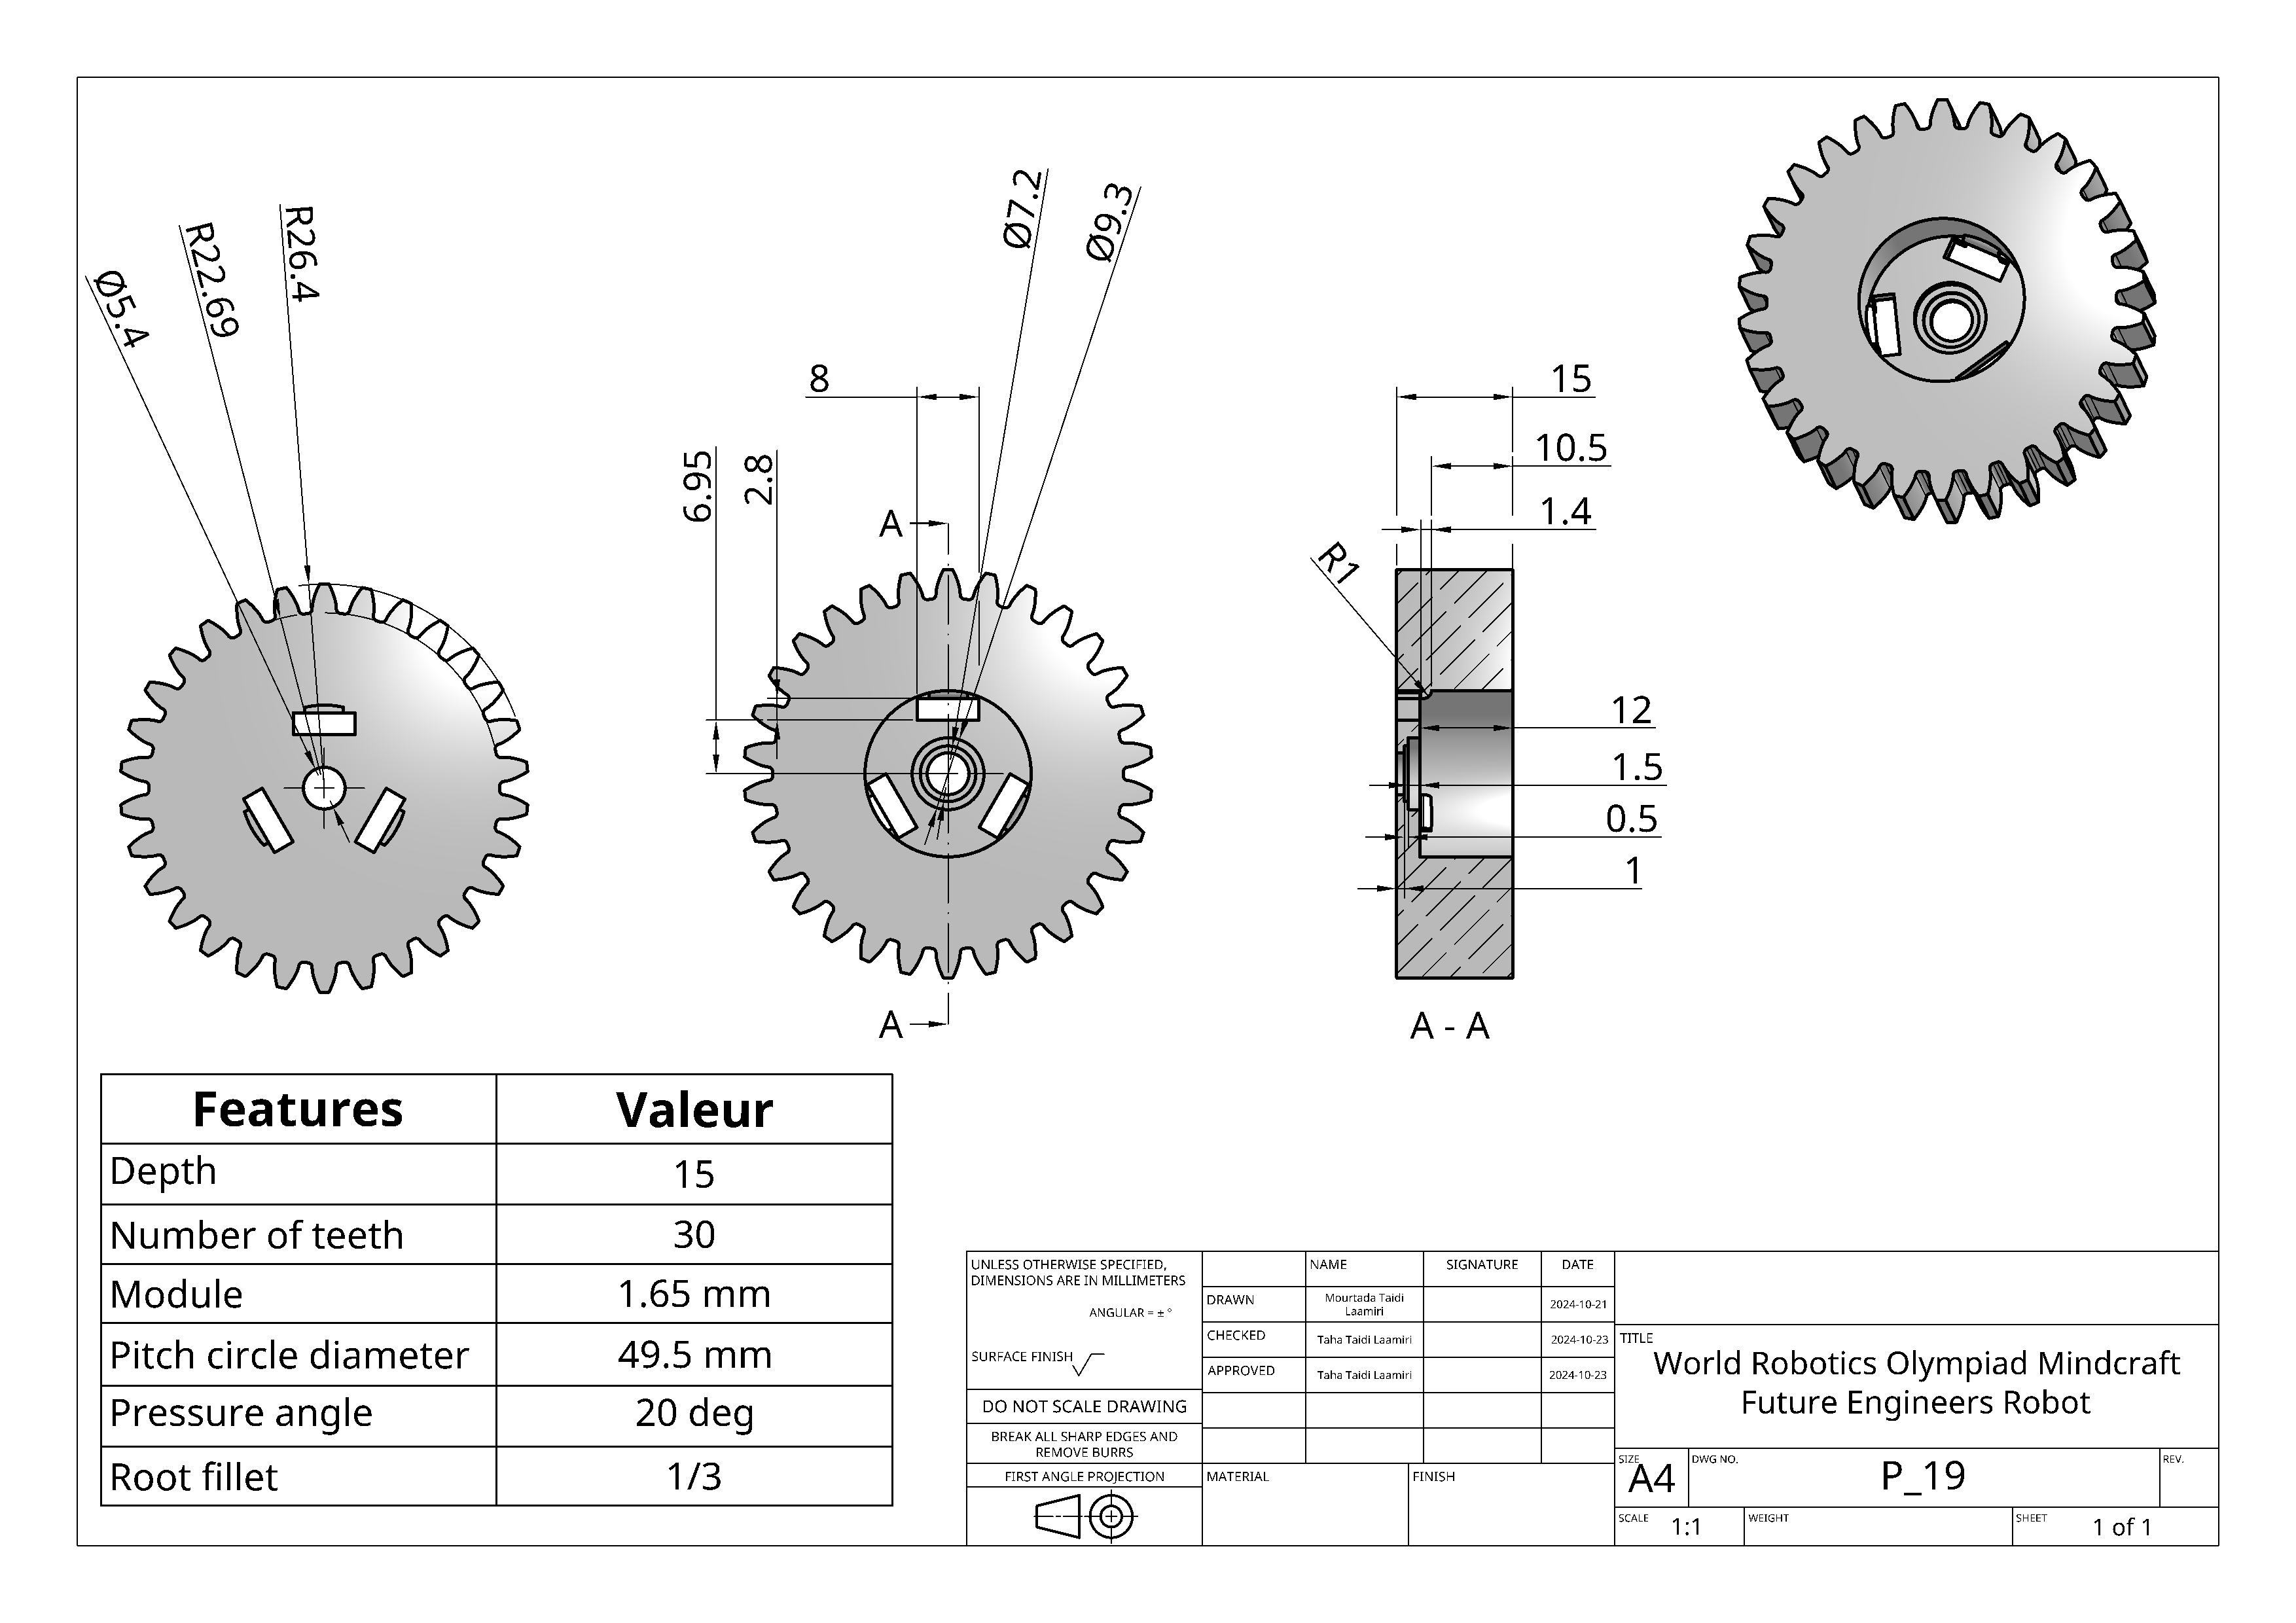
\includegraphics[width=\textwidth, angle=90]{figures/Drawing/Drawing Big Gear.png}
    \caption{Big Gear}
\end{figure}

\begin{figure}[H]
    \vspace{4cm}
    \centering
    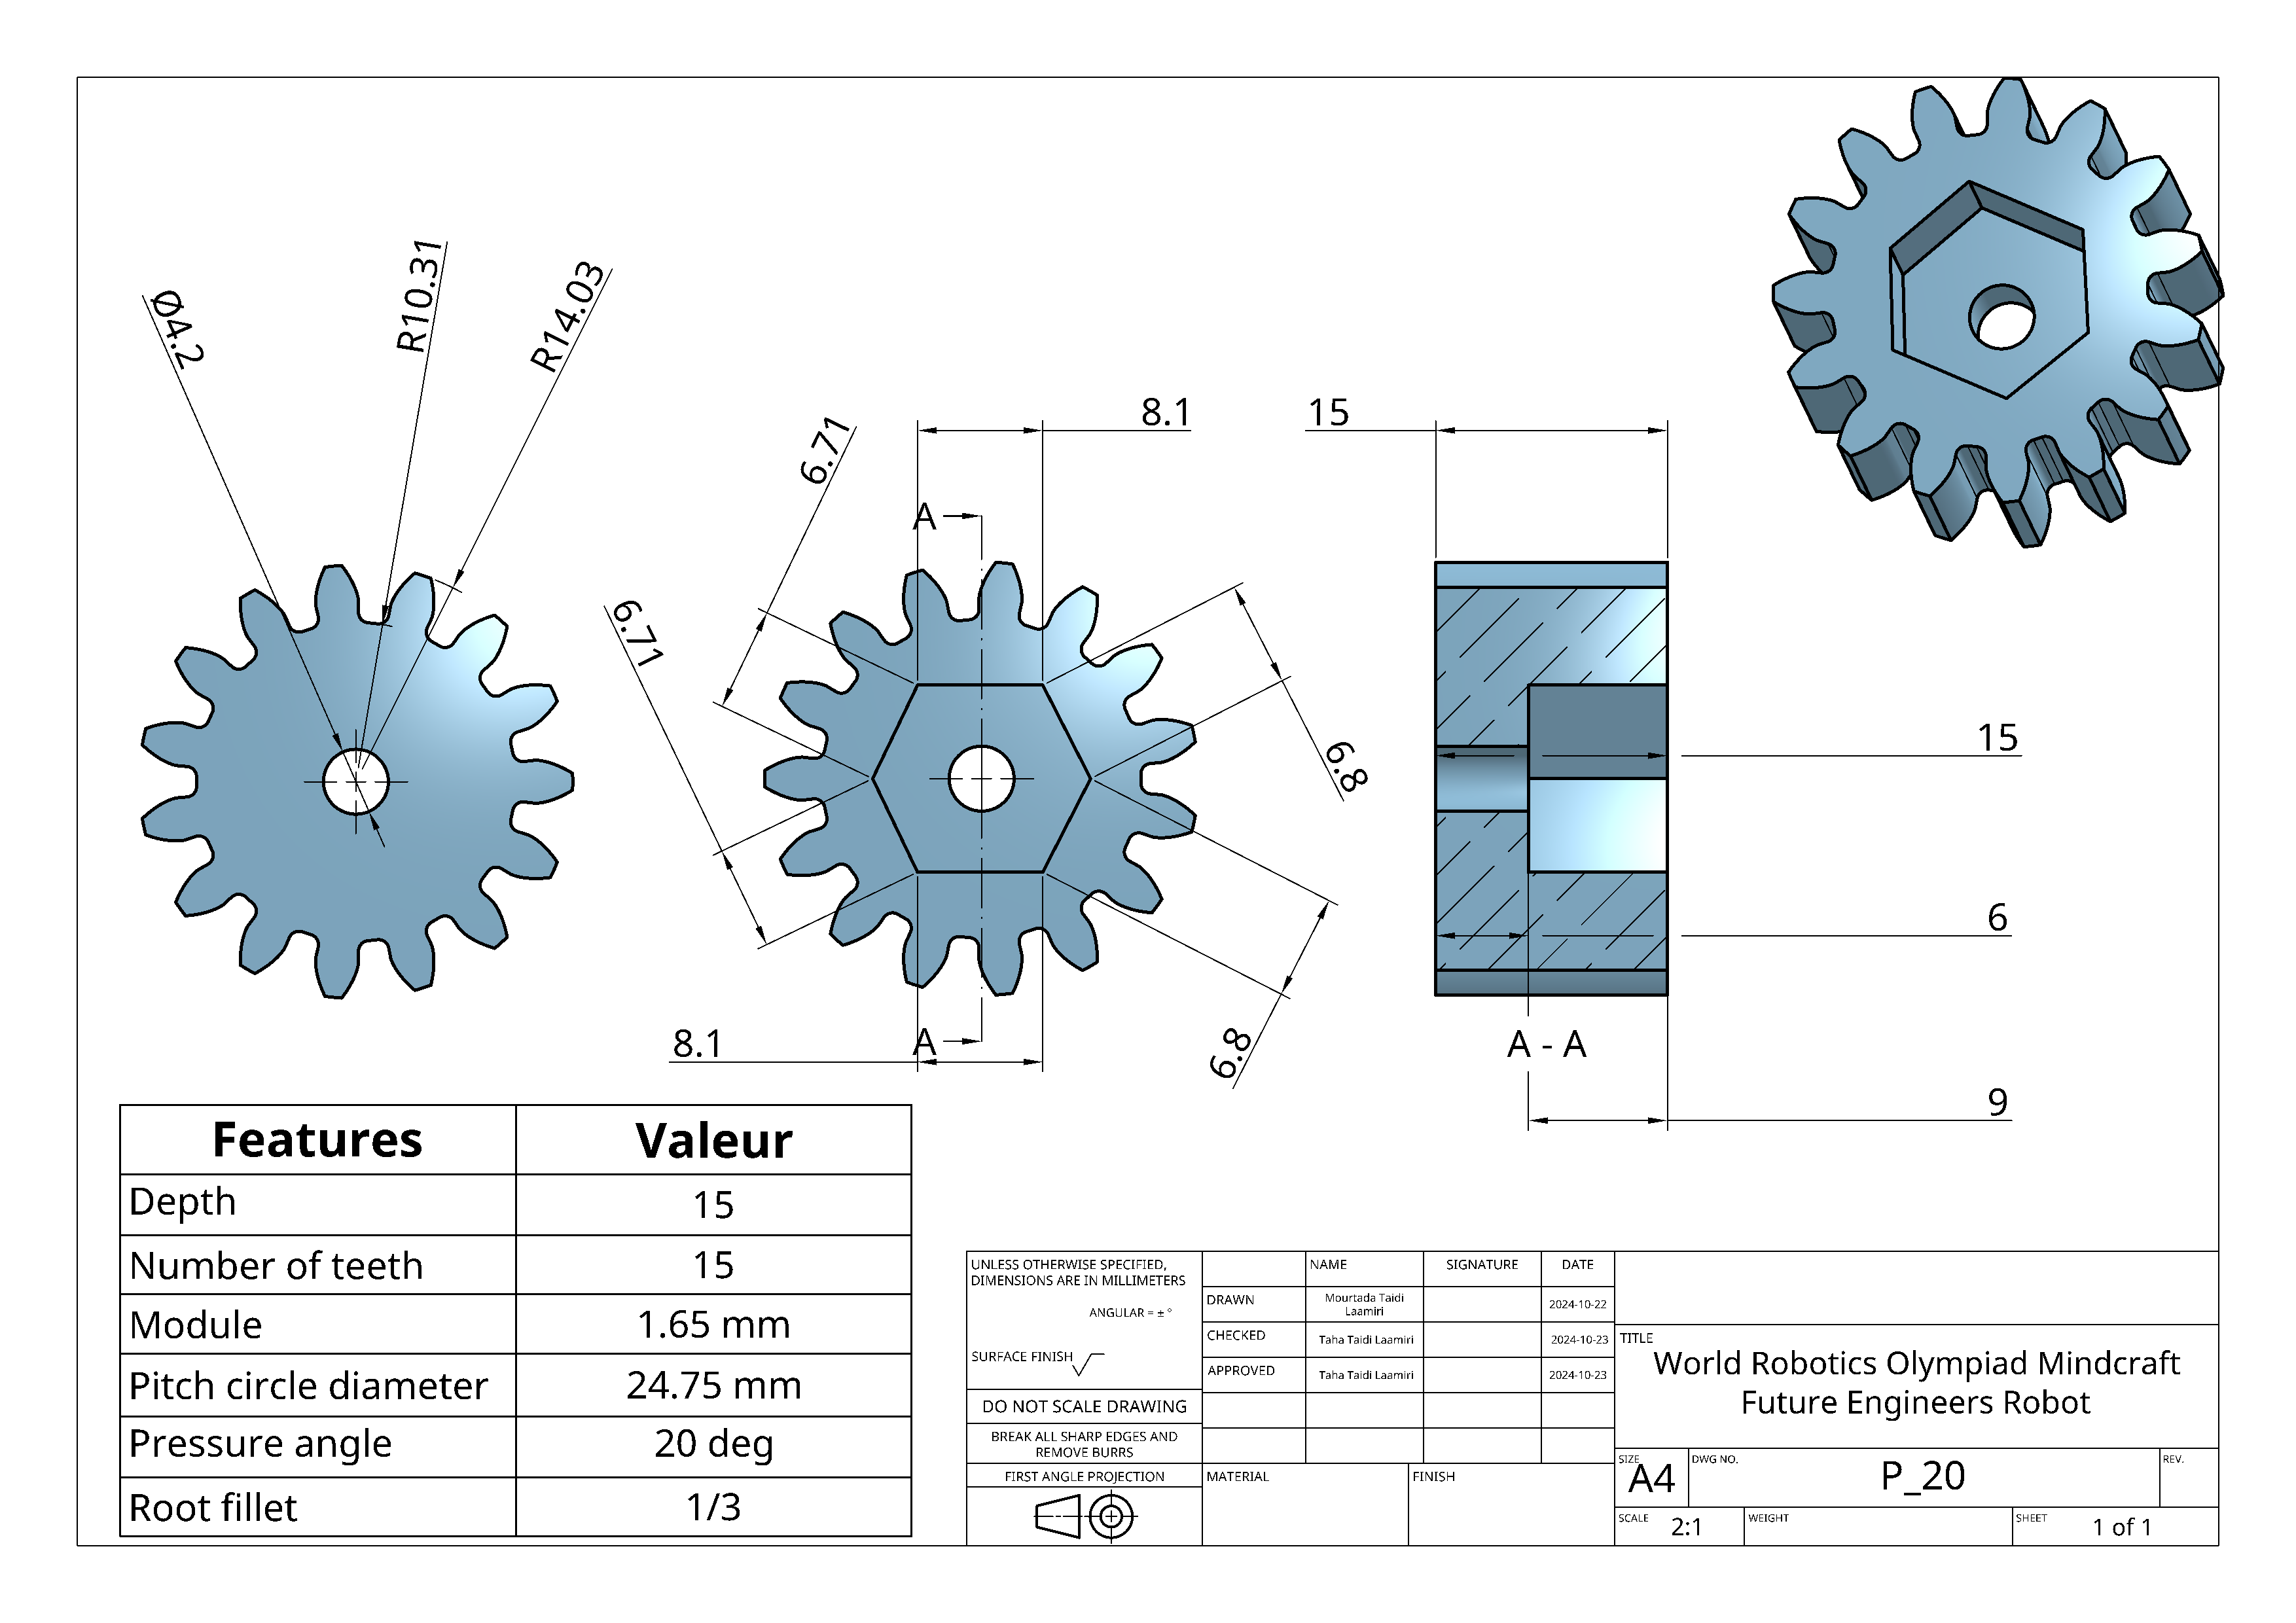
\includegraphics[width=\textwidth, angle=90]{figures/Drawing/Drawing Gear.png}
    \caption{Gear}
\end{figure}

\begin{figure}[H]
    \vspace{4cm}
    \centering
    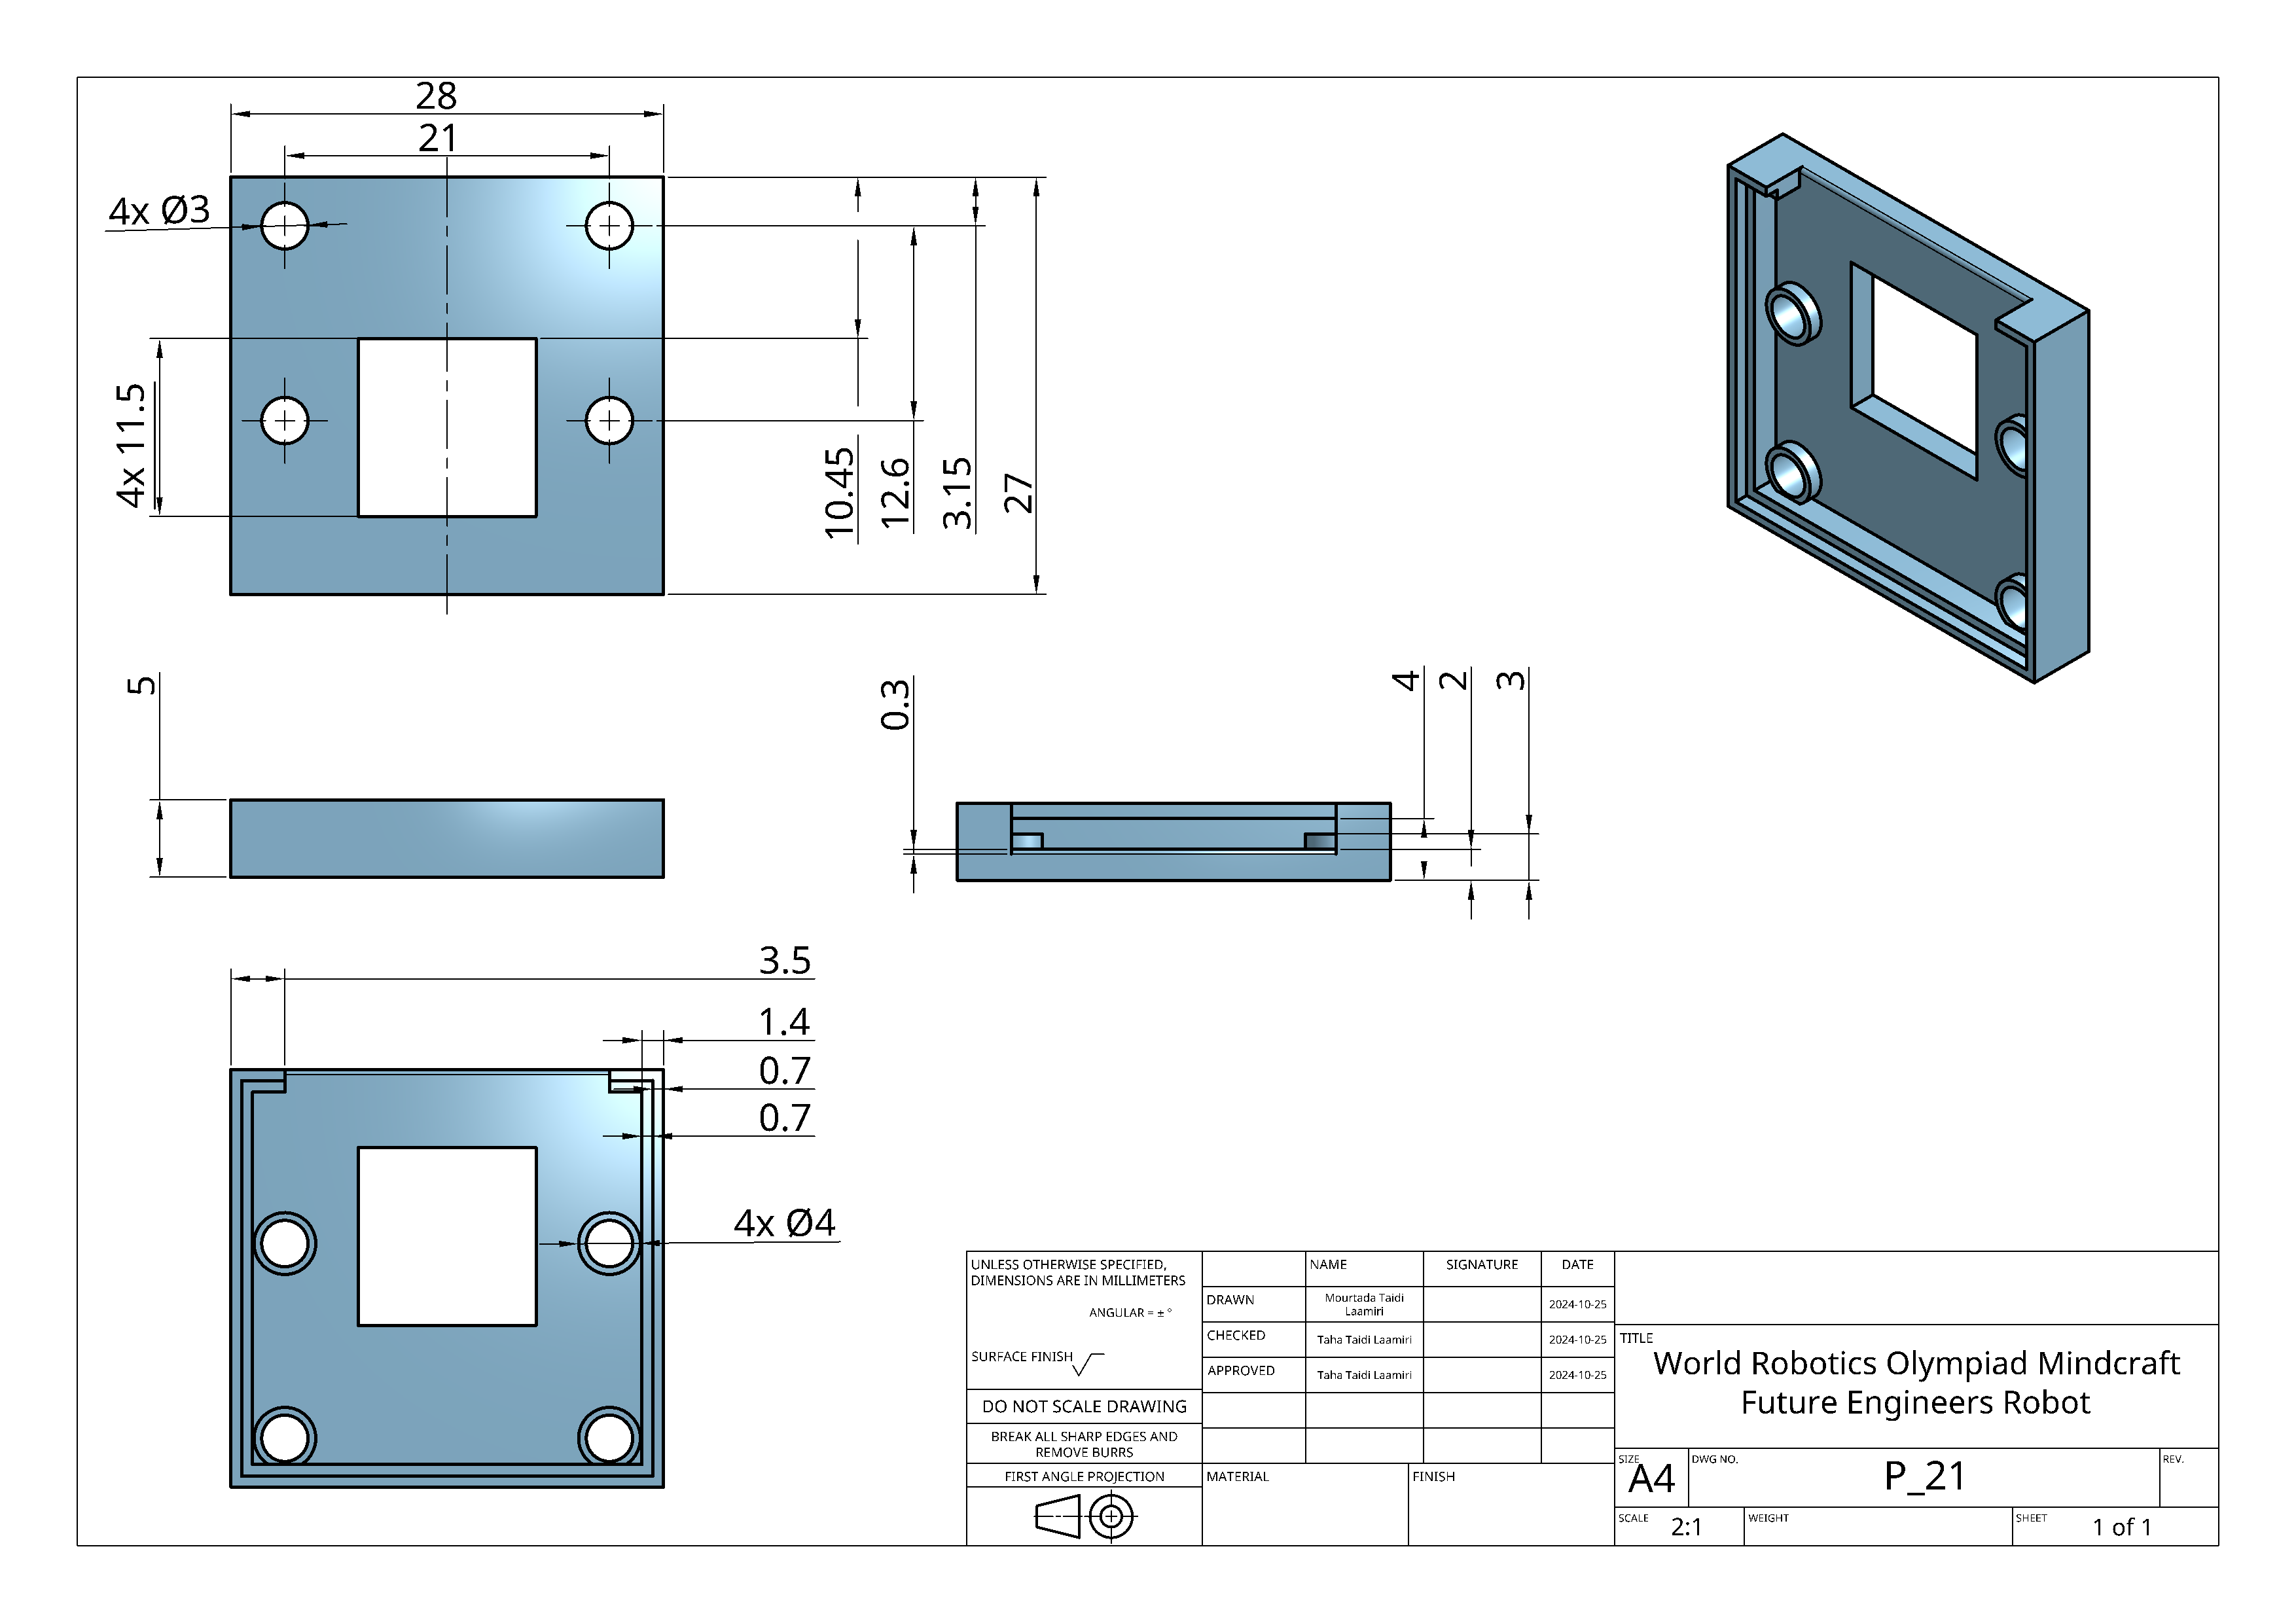
\includegraphics[width=\textwidth, angle=90]{figures/Drawing/Drawing Front Support Camera.png}
    \caption{Front Support Camera}
\end{figure}

\begin{figure}[H]
    \vspace{4cm}
    \centering
    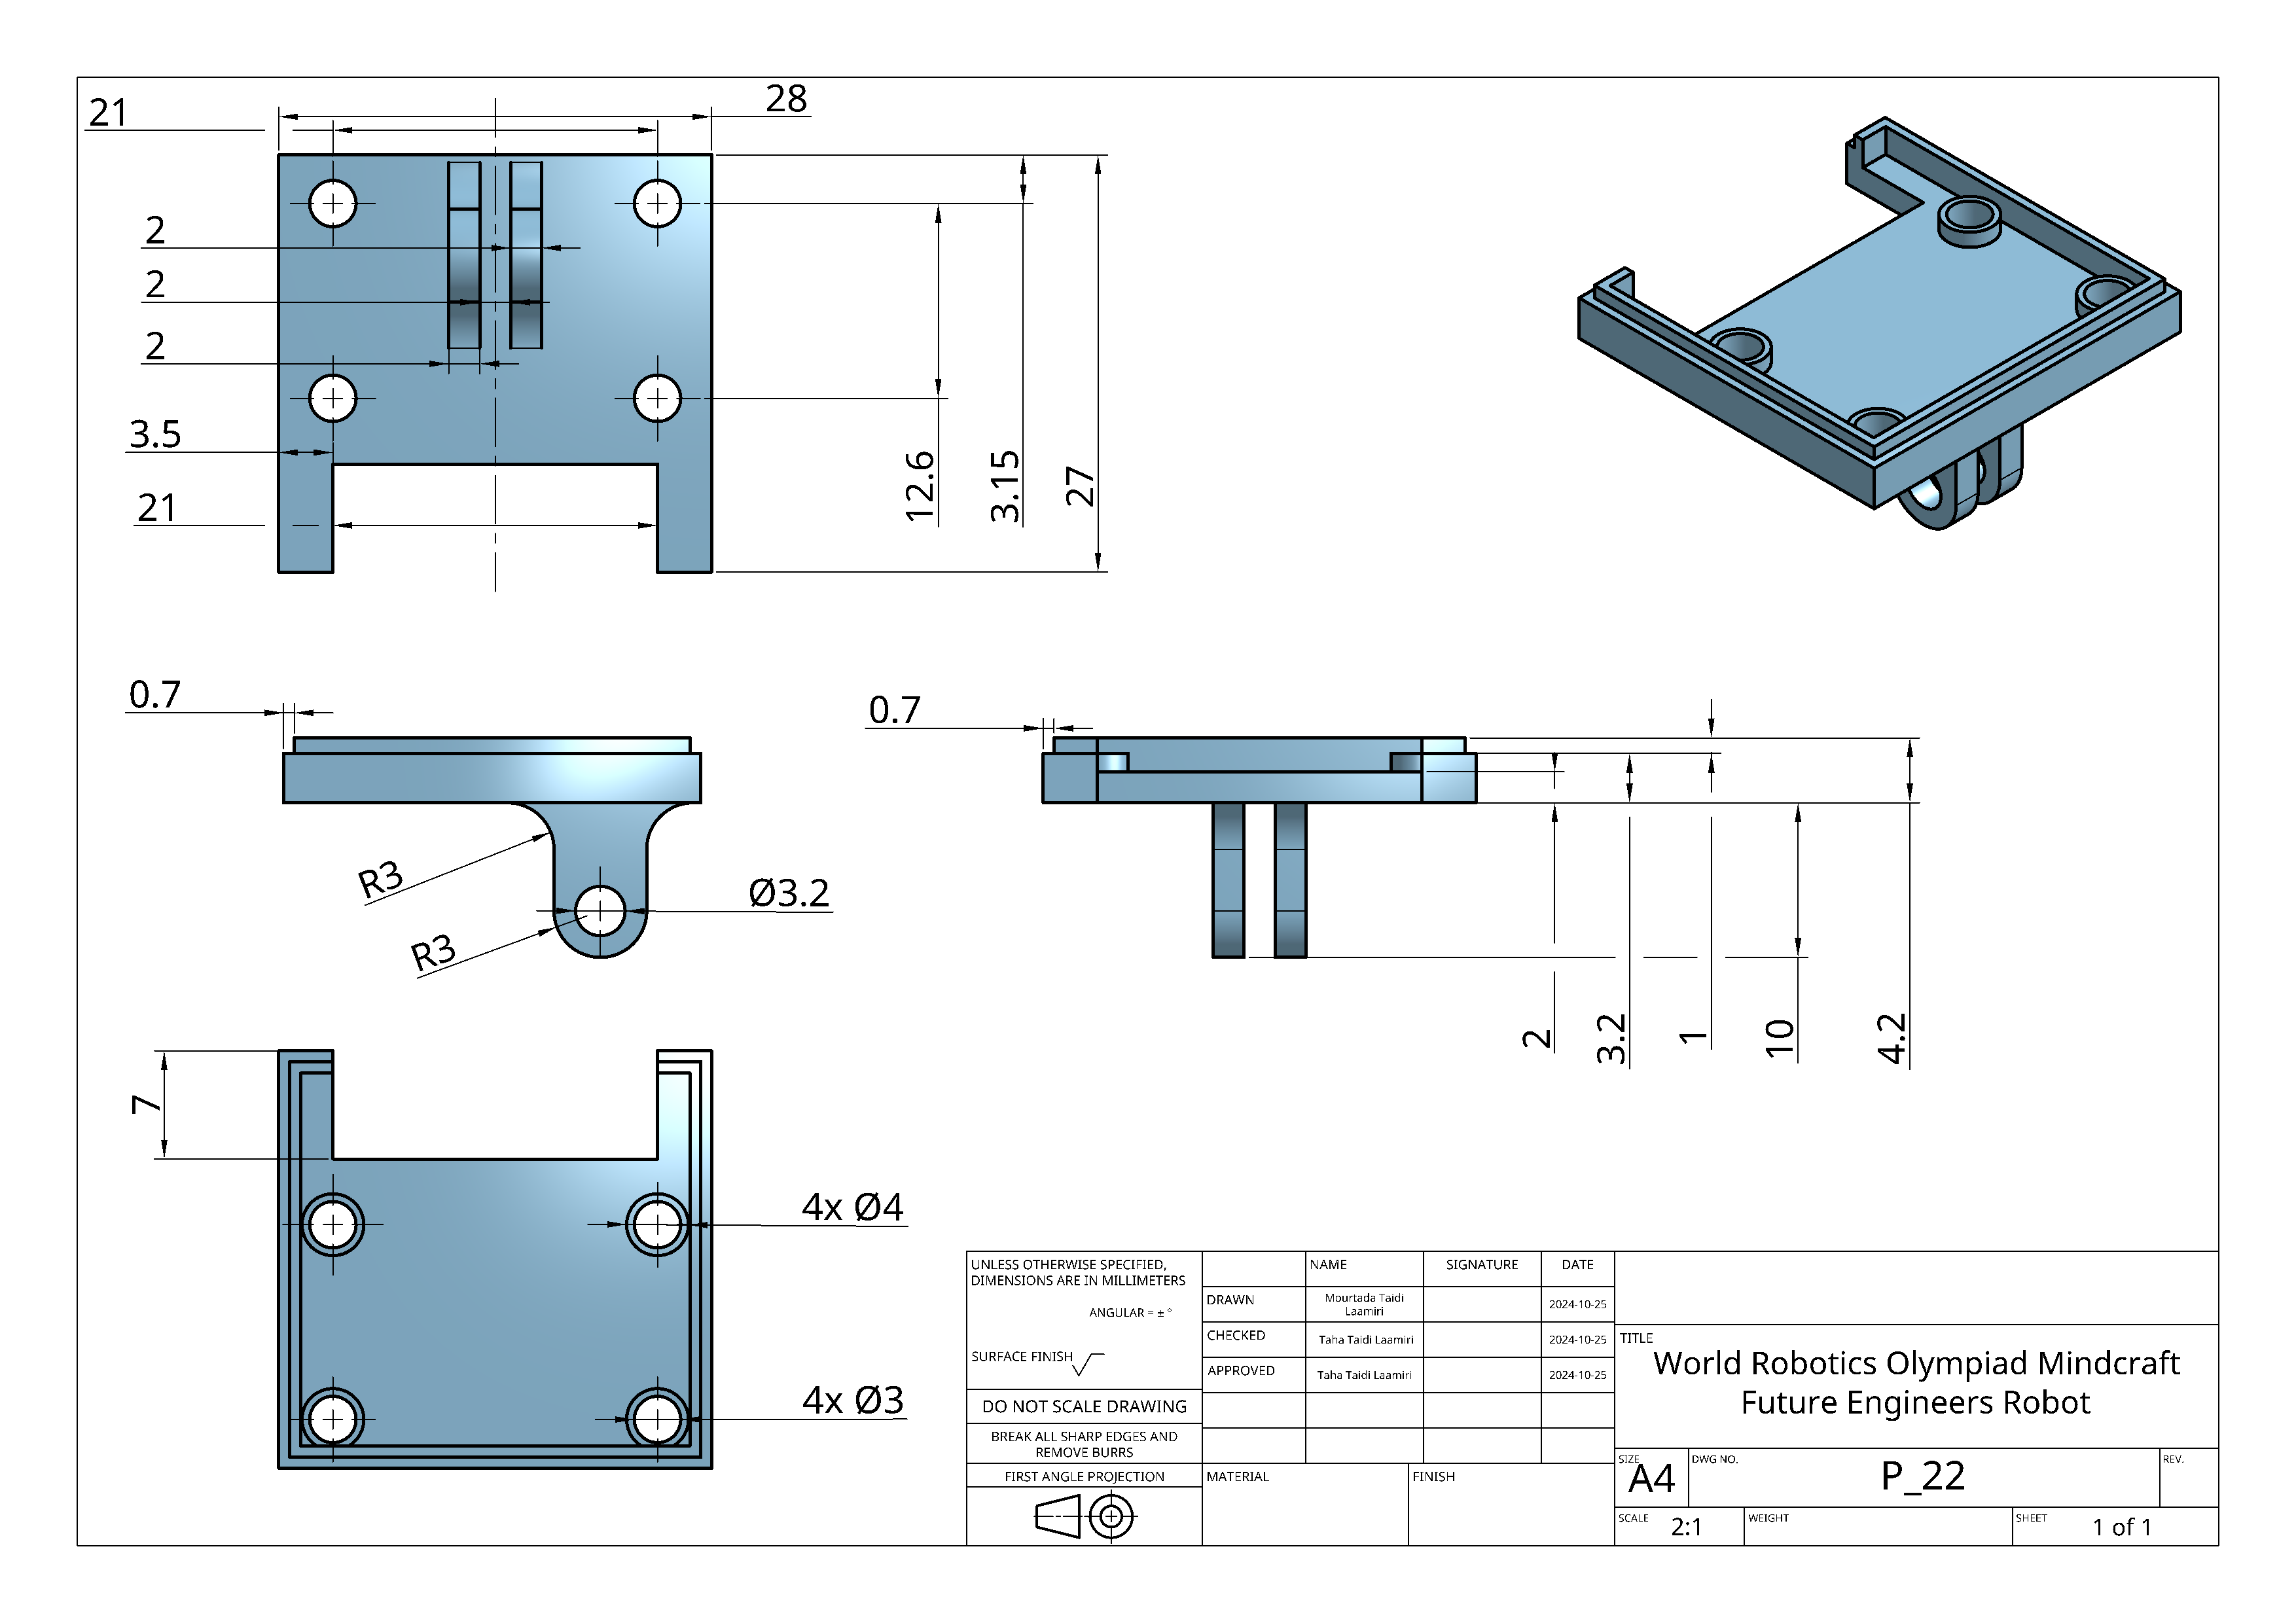
\includegraphics[width=\textwidth, angle=90]{figures/Drawing/Drawing Back Support Camera.png}
    \caption{Back Support Camera}
\end{figure}

\begin{figure}[H]
    \vspace{4cm}
    \centering
    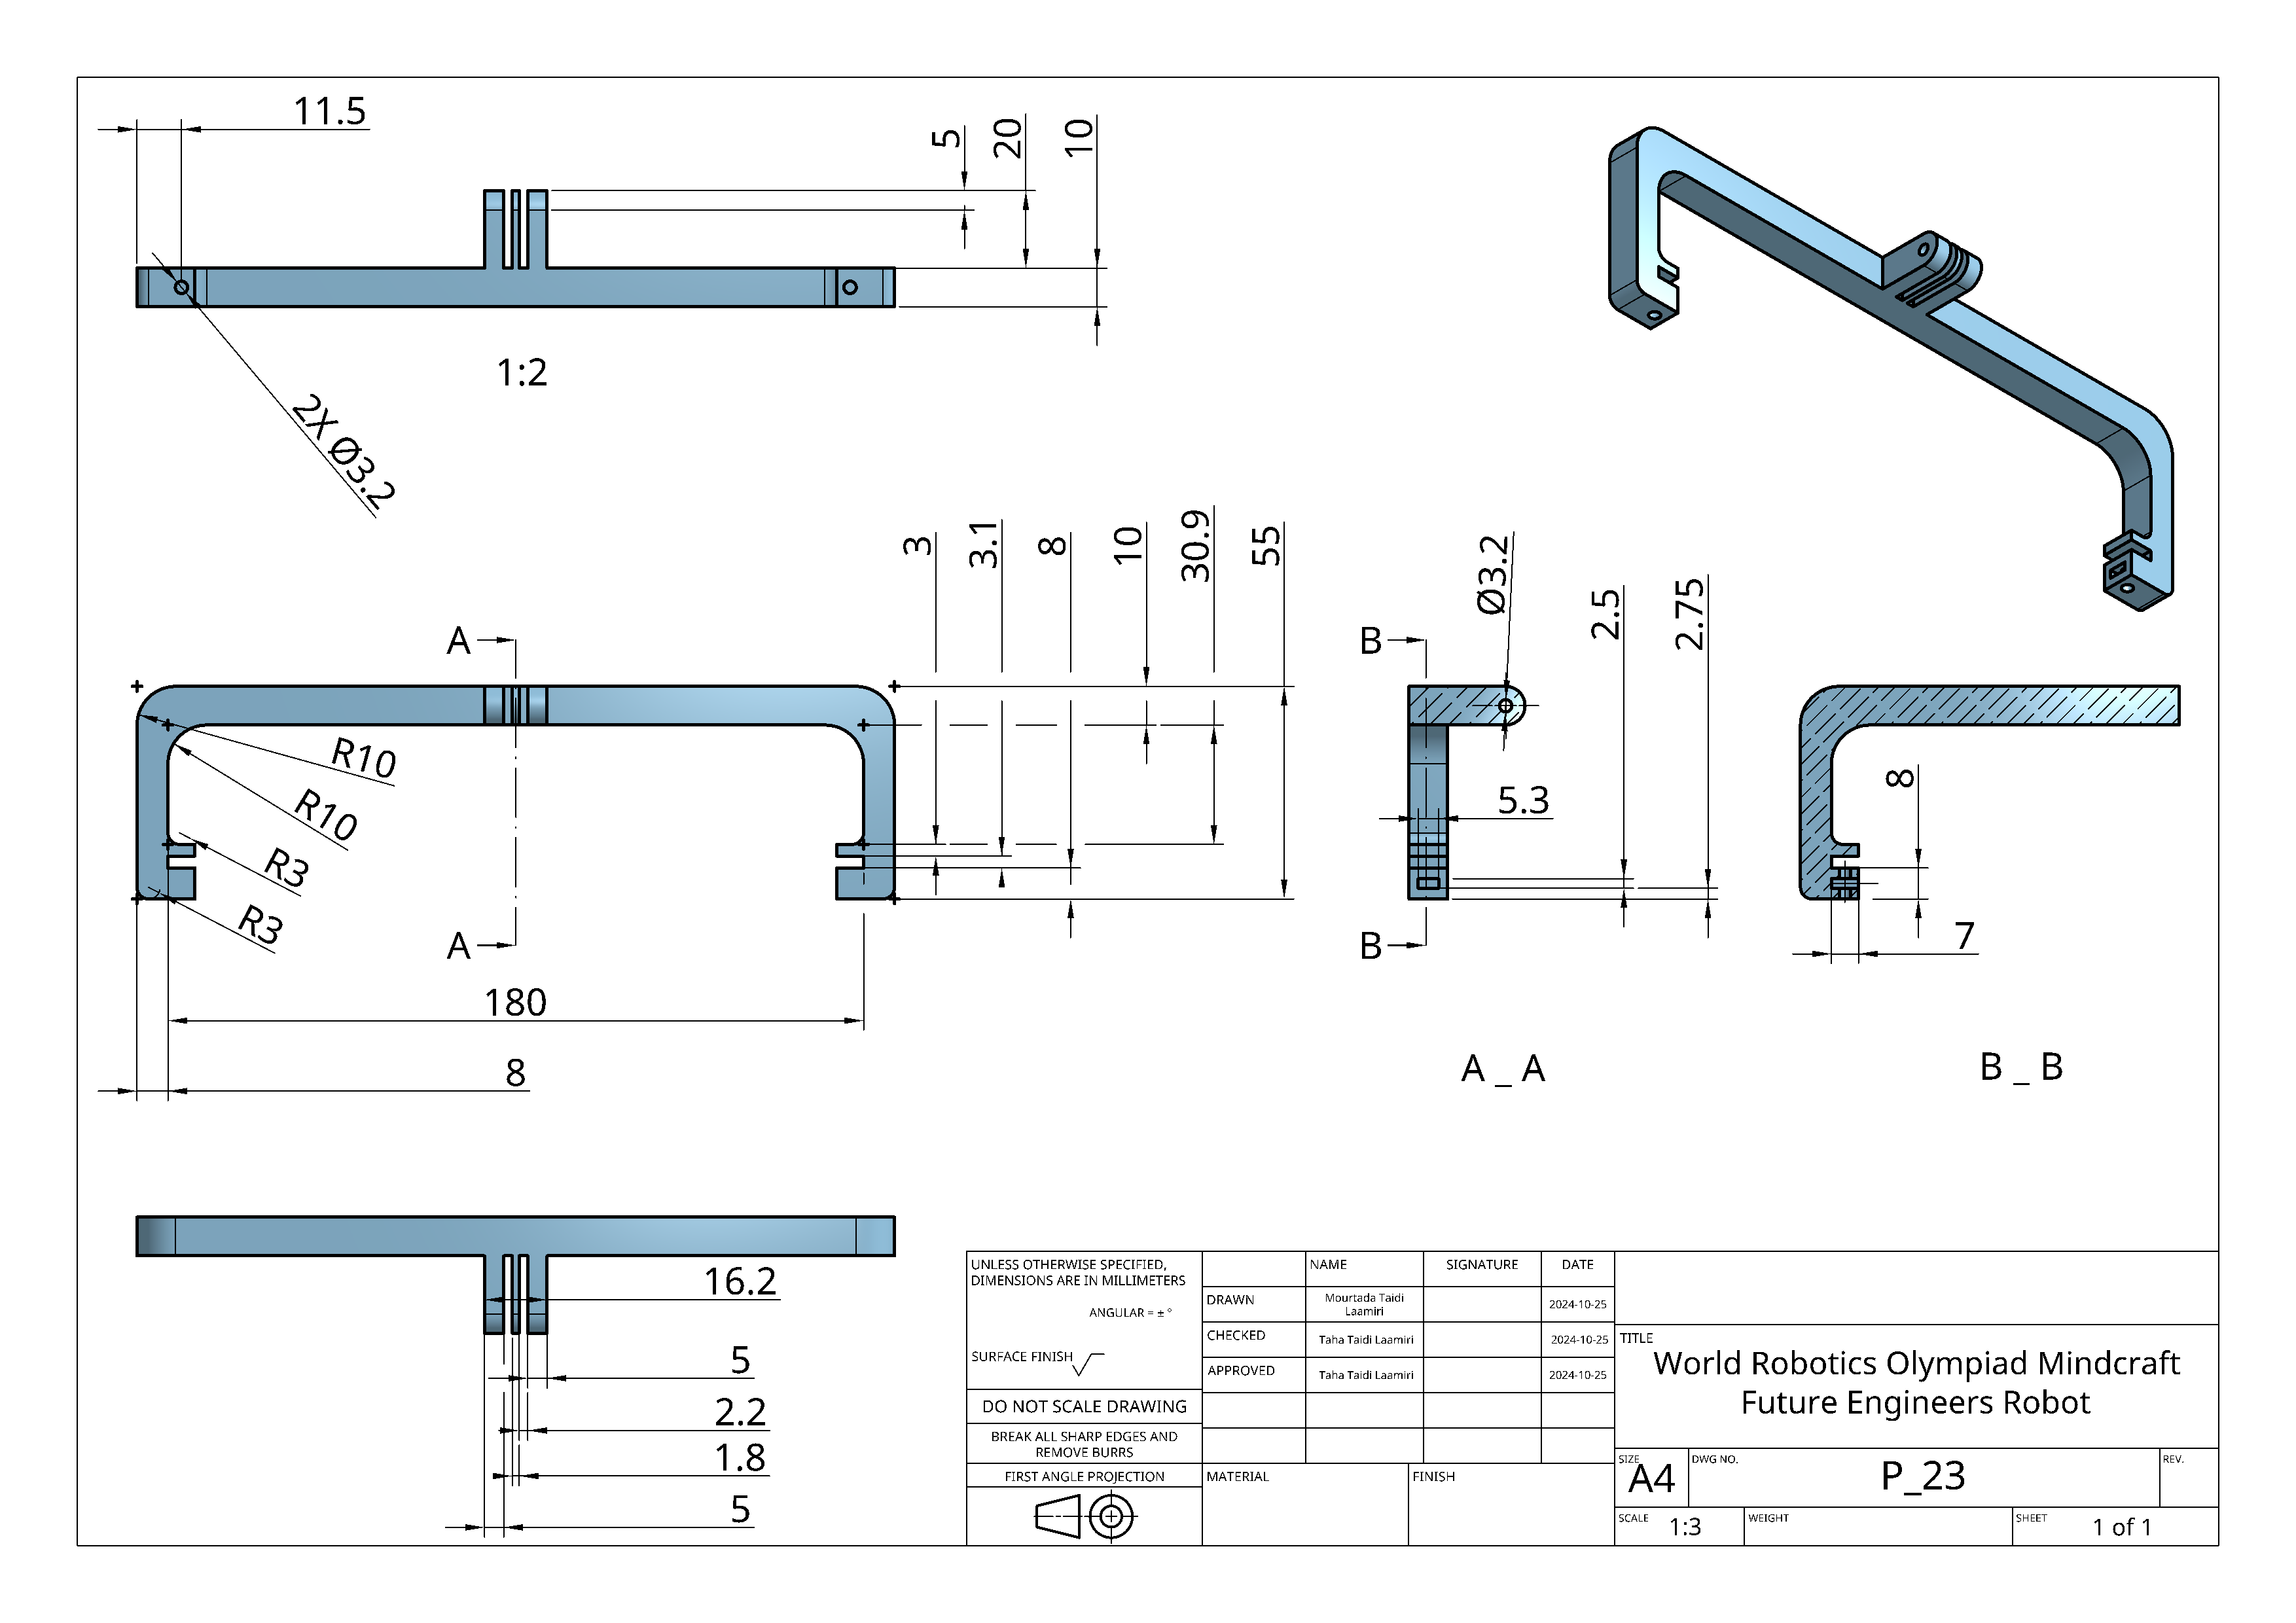
\includegraphics[width=\textwidth, angle=90]{figures/Drawing/Drawing Conector Support Camera.png}
    \caption{Conector Support Camera}
\end{figure}





\newpage

\section{Electrical Components and Integration}
The robot's electrical system comprises various components working together to achieve efficient and autonomous operation. This section describes the purpose and role of each electrical part, along with its integration into the overall design.


\subsection{Schemes}
\begin{figure}[H]
    \centering
    \includegraphics[width=1\linewidth]{figures/scheme.png}
    \caption{Electrical Diagram}
    \label{fig:scheme}
\end{figure}

\subsection{Raspberry Pi 4B}
\begin{itemize}
    \item \textbf{Purpose}: The Raspberry Pi 4B serves as the central processing unit (CPU) for the robot, running the control algorithms, ROS2 Humble, and real-time data processing from sensors.
    \item \textbf{Specifications}: Quad-core Cortex-A72, 8GB RAM, USB 3.0 ports, and micro-HDMI output.
    \item \textbf{Integration}: It interfaces with sensors, motor drivers, and peripherals via GPIO, I2C, and USB ports, providing the computational power for vision and navigation.
\end{itemize}
\newpage



\subsection{RPLIDAR C1 (LIDAR Sensor)}
\begin{itemize}
    \item \textbf{Purpose}: The LIDAR sensor is used for mapping the environment, detecting obstacles, and enabling precise navigation through SLAM (Simultaneous Localization and Mapping).
    \item \textbf{Specifications}: 360-degree scanning range, up to 8m distance, 8000 samples per second.
    \item \textbf{Integration}: Connected to the Raspberry Pi via USB, the data is processed using ROS2 packages for real-time mapping and obstacle detection.
\end{itemize}

\subsection{Arduino Nano}
\begin{itemize}
    \item \textbf{Purpose}: The Arduino Nano acts as a secondary microcontroller for handling low-level tasks such as motor control and sensor data acquisition.
    \item \textbf{Specifications}: ATmega328P microcontroller, 14 digital I/O pins, and I2C compatibility.
    \item \textbf{Integration}: Communicates with the Raspberry Pi over I2C, relaying data from sensors like the MPU6050 and VL53L0X DTOF sensors.
\end{itemize}

\subsection{VL53L0X DTOF Sensors (x4)}
\begin{itemize}
    \item \textbf{Purpose}: These sensors measure distances to obstacles with high precision, providing data for collision avoidance and path correction.
    \item \textbf{Specifications}: Measurement range of up to 2m, high-accuracy Time-of-Flight technology.
    \item \textbf{Integration}: Positioned on each side of the robot, connected via I2C, and managed by the Arduino Nano for fast response times.
\end{itemize}

\subsection{MPU6050 (Gyroscope and Accelerometer)}
\begin{itemize}
    \item \textbf{Purpose}: The MPU6050 provides orientation and motion data, critical for maintaining stability and correcting drift.
    \item \textbf{Specifications}: 3-axis gyroscope and 3-axis accelerometer.
    \item \textbf{Integration}: Data is processed by the Arduino Nano and sent to the Raspberry Pi for real-time corrections.
\end{itemize}

\subsection{Pi Camera (PiCam V2)}
\begin{itemize}
    \item \textbf{Purpose}: Captures video feed for lane detection, cube identification, and object tracking.
    \item \textbf{Specifications}: 8MP resolution, 1080p video recording.
    \item \textbf{Integration}: Mounted on a 3D-printed bracket, the camera interfaces directly with the Raspberry Pi for real-time image processing.
\end{itemize}

\subsection{Motor Driver (L298N) and Motors}
\begin{itemize}
    \item \textbf{Purpose}: Controls the robot’s four-wheel drive system, enabling forward, backward, and differential motion.
    \item \textbf{Specifications}: Dual H-bridge motor driver with PWM support.
    \item \textbf{Integration}: Receives PWM signals from the Arduino Nano and drives the DC motors.
\end{itemize}

\subsection{Battery and Power Management}
\begin{itemize}
    \item \textbf{Purpose}: Provides power to all components, including the Raspberry Pi, sensors, and motors.
    \item \textbf{Specifications}: 12V 5000mAh LiPo battery.
    \item \textbf{Integration}: Managed through a custom power distribution board with safety fuses and voltage regulators.
\end{itemize}

\newpage

\section{Software and Coding}
The software infrastructure is built on ROS2 Humble, leveraging various libraries and tools for real-time robot operation.

\subsection{ROS2 Humble}
\begin{itemize}
    \item \textbf{Purpose}: Provides a modular framework for robotics applications, handling sensor integration, navigation, and control.
    \item \textbf{Features Used}:
    \begin{itemize}
        \item Navigation2: Path planning and obstacle avoidance.
        \item Sensor Fusion: Integrates LIDAR, camera, and DTOF data.
        \item RCLPy: Python-based ROS client library for custom scripts.
    \end{itemize}
\end{itemize}

\begin{figure}[ht]
    \centering
    \includegraphics[width=0.5\textwidth]{figures/ros2.png}
    \caption{ROS2 Logo.}
    \label{fig:ros2}
\end{figure}

\subsection{RPLIDAR C1 Integration}
\begin{itemize}
    \item \textbf{Purpose}: Enables SLAM for environment mapping and obstacle detection.
    \item \textbf{Implementation}: The LIDAR data is processed using the ROS2 slam toolbox package, creating a dynamic map of the environment.
\end{itemize}

\begin{figure}[H]
    \centering
    \includegraphics[width=1\linewidth]{figures/rviz2.png}
    \caption{Rplidar Visualization using rviz2}
    \label{fig:rviz2}
\end{figure}

\subsection{Pi Camera (PiCam V2) and OpenCV}
\begin{itemize}
    \item \textbf{Purpose}: Used for visual processing tasks, including lane detection and object recognition.
    \item \textbf{Implementation}: OpenCV handles image preprocessing, edge detection, and color filtering, integrated with ROS2 nodes for real-time control.
\end{itemize}

\subsection{Dashboard}
\begin{itemize}
    \item \textbf{Purpose}: Provides a live interface for monitoring robot performance and issuing commands.
    \item \textbf{Tools Used}: Tkinter framework for the backend, integrated with ROS2.
    \item \textbf{Features}: Real-time sensor data visualization, camera feed display, and remote control options.
\end{itemize}

\newpage

\section{Strategy and Autonomous Behavior}
The robot's strategy focuses on efficient pathfinding, obstacle avoidance, and task completion.

\subsection{Pathfinding and Navigation}
The robot uses data from LIDAR and DTOF sensors for precise navigation. SLAM enables it to dynamically map the course, ensuring efficient path selection.

\subsection{Obstacle Avoidance}
Sensors like LIDAR, DTOF, and the Pi Camera work together to identify and avoid obstacles. A layered costmap from ROS2 Navigation2 ensures safe paths are planned in real-time.

\subsection{Task-Specific Behaviors}
\begin{itemize}
    \item **Cube Identification**: The robot identifies cubes using the Pi Camera and avoids them during navigation.
    \item **Lane Following**: OpenCV processes the camera feed to detect and follow lanes on the track.
    \item **Dynamic Adjustments**: The robot adjusts speed and direction based on sensor feedback, ensuring smooth operation.
\end{itemize}

\begin{figure}
    \centering
    \includegraphics[width=1\linewidth]{Flowchart (3).pdf}
    \caption{Open Challenge Strategy.}
    \label{fig:open}
\end{figure}

\newpage

\begin{figure}
    \centering
    \includegraphics[width=1\linewidth]{figures/Flowchart (2).pdf}
    \caption{Obstacle Challenge Strategy.}
    \label{fig:obstacle}
\end{figure}

\newpage


\subsection{Randomizer & Score Calculator}
\begin{itemize}
    \item \textbf{Purpose}: Offering an online open-source website that randomizes the map and calculates the score.
    \item \textbf{Implementation}: Using HTML, CSS for forend, and JavaScript for Backend.
    \item \textbf{Using}: Used Github Pages to build and upload the website.
\end{itemize}

\begin{figure}[ht]
    \centering
    \includegraphics[width=1\linewidth]{figures/randomizer.png}
    \caption{Part of JavaScript Code.}
    \label{fig:JS}
\end{figure}


\newpage

\section{Links}

\subsection{Youtube Channel}
\vspace{0.5cm}
\qrcode[height=4cm]{https://www.youtube.com/@MindcraftWRO-kw8vp}
\vspace{1cm}

\subsection{Github Repository}
\vspace{0.5cm}
\qrcode[height=4cm]{https://github.com/DexterTaha/WRO-FE-2024-Mindcraft-International}
\vspace{1cm}

\subsection{Onshape Link}
\vspace{0.5cm}
\qrcode[height=4cm]{https://cad.onshape.com/documents/1c6f1405e84d0c390333223c/w/c90b719cdc670bdbfb16a84e/e/3d798daea79d75d88b470c18?renderMode=0&uiState=671bdafd0e6bd205bc48c042}

\newpage
\end{document}